 %% Copyright (C) 2006 Ahmer Ahmedani

\documentclass[MSc,twoside,openright]{Thesis}

\newif\ifdraft
% \drafttrue

%== Preamble ==================================================================

\usepackage[french]{babel}
\usepackage[T1]{fontenc}
\usepackage[utf8]{inputenc}

\usepackage{algorithm}
\usepackage{algpseudocode}
\usepackage{placeins}
\usepackage{tabularx}
\usepackage{multicol}
\usepackage{xcolor}    % Keyword highlighting in listing
\usepackage{listings}  % Typeset source code listings,
                       % Files in current direcotry
                       % ( listings.cfg listings.sty lstdoc.sty lstlang1.sty
                       % lstlang2.sty lstlang3.sty lstmisc.sty ) are listings
                       % version 1.4, should not be removed, 1.3 version cause
                       % problem in the left line of the frame (standalone use 
                       % of 1.3 will not cause this problem, but in this
                       % project, it does)
\usepackage[bw]{mcode} % mcode listings
\usepackage{x10}			 % x10 listings	
\usepackage{ifthen}    % For conditional commands
\usepackage{ifpdf}     % Provide \ifpdf conditional
\usepackage{xspace}    % Define commands that don't eat spaces
\usepackage{type1cm}
\usepackage{times}     % Use Times *deprecated*
%% listings.sty doesn't seem to pretty print code listings if the
%% `times' packages is not loaded. Why? Who knows. It will do it fine
%% in a simple document, just not in this one.
\usepackage{mathptmx}  % Use Times for roman family and math
% \usepackage{mathpazo}  % Palantino
% \usepackage{chancery}
% \usepackage{bookman}
% \usepackage{newcent}
% \usepackage{charter}
\usepackage[scaled]{helvet}    % Use Helvetica for sans serif family
%\usepackage{avant}     % Use Avant Garde for sans serif family
\usepackage{pifont}    % Symbol and Zapf Dingbats
%% TODO: investigate fourier package (Adobe Utopia fonts)

\usepackage{fancyhdr}  % Fancy page headers
\usepackage{verbatim}  % provide comment environments
\usepackage{fancyvrb}  % improved verbatim and verbatim* environments

%\usepackage{hyperref} % split urls
\usepackage{url}       % For nicely formatted URLs


%% Nicer formatting of figure captions:
\usepackage[format=hang,font={small,sf},labelfont=bf,labelsep=space]{caption}
%\usepackage[tight]{subfigure} % subfigures. replace with subfig?
\usepackage{subfig}
\usepackage{setspace}
\usepackage{longtable} % Make tables span multiple pages
\usepackage{multirow}  % Table cells that span multiple rows
\usepackage{dcolumn}   % Line up decimal sep in tabular columns
% \usepackage{warpcol}   % Alternate to dcolumn
\usepackage{color}     % Allows text and page background colors to be set
\usepackage{colortbl}  % Coloured tables
\usepackage[final]{graphicx}  % Better support for graphics
\usepackage{layout}    % produces a figure that describes the page layout
\usepackage{titlesec}  % to redefine typesetting of \paragraph
\usepackage{rotating}  % for rotated table headings
% Note: yap does not support rotating, so convert .dvi to .pdf and then
%    preview the .pdf file
% for algorithms
%\usepackage[algo2e, algochapter, ruled, linesnumbered, lined]{algorithm2e}
%% Make sure that the bibliography is listed in the table of contents,
%% but that the table of contents itself is not.
% XXX: doesn't seem to work
%\usepackage[nottoc]{tocbibind} 
\usepackage[none]{tocbibind}
%\usepackage{hyphenat} %enhanced hyphenation, 
%\usepackage[htt]{hyphenat} %htt enables hyphenation of text typeset
% some better colours for hyperref links:
\definecolor{darkgreen}{rgb}{0.2,0.5,0.1}
\definecolor{darkblue} {rgb}{0.1,0.4,0.5}
\definecolor{maroon}   {rgb}{0.45,0.05,0.25}
\definecolor{red}      {rgb}{1,0,0}
\ifpdf
  %% TODO: can I use variables here for name, title, etc?
  \usepackage[
    pdftex,
    colorlinks=true,
    linkcolor=maroon,
    citecolor=darkgreen,
    pagecolor=maroon,
    urlcolor=darkblue,
    pdftitle={The MetaLexer Lexer Specification Language},
    pdfauthor={Andrew Casey},
    pdfsubject={The MetaLexer Lexer Specification Language},
    pdfkeywords={MetaLexer, Lexer, Scanner, Extensible, Modular}
  ]
  {hyperref} % hyper-text links, etc.
\else
  \usepackage[
    dvips,
    breaklinks=true,
    colorlinks=true,
    linkcolor=maroon,
    citecolor=darkgreen,
    pagecolor=maroon,
    urlcolor=darkblue,
  ]
  {hyperref}
\fi


% Use the ams math packages
\usepackage{amssymb,amsmath}

% tell LaTeX where to find find figures
%\ifpdf
%  \DeclareGraphicsExtensions{.pdf,.jpg,.png}
%  \graphicspath{{images/}}
%\else
%  \DeclareGraphicsExtensions{.eps,.ps}
%  \graphicspath{{images/}}
%\fi

\usepackage{bnf}




% -- Customize Layout ---------------------------------------------------------

% custom page headers:

\lhead[]{\fancyplain{}{\nouppercase{\rightmark}}}
\rhead[\fancyplain{}{\nouppercase{\leftmark}}]{}
\addtolength{\headwidth}{10mm} % => extend line out into margin

%\fancyhead[EL]{THESIS DRAFT}
%\fancyhead[OR]{THESIS DRAFT}


\titleformat{\paragraph}[hang]{\normalfont\it}{}{0em}{}

% Make LaTeX relax a little wrt figure placement
\renewcommand{\topfraction}{0.85}
\renewcommand{\textfraction}{0.1}
\renewcommand{\floatpagefraction}{0.75} % Prevent half-empty pages

\newcommand*\justify{%
  \fontdimen2\font=0.4em% interword space
  \fontdimen3\font=0.2em% interword stretch
  \fontdimen4\font=0.1em% interword shrink
  \fontdimen7\font=0.1em% extra space
  \hyphenchar\font=`\-% allowing hyphenation
}

% Tell LaTeX to not "bottom justify" text. This prevents ugly
% spaces between paragraphs in columns when LaTeX stretches them.
\raggedbottom

% Set the depth for the table of contents to 2 for non-draft output
\ifdraft
\else
\setcounter{tocdepth}{2}
\fi



\algnewcommand{\Lcomment}[1]{\State \(\triangleright\){\color{gray}{\footnotesize
\textit {#1}}}}
%\ifdraft
%  \pagestyle{myheadings} \markright{Draft \today: Please do not 
%  redistribute.}
%\else
%  \pagestyle{headings}
%\fi

% Set the value of the margin of all algorithms.
% The default value is \leftskip plus \parindent 
%  when the algorithm2e package is loaded. 
%\incmargin{\parindent} %increase one more \parindent to the default 
% Set font of comment in algorithms
\algnewcommand{\algcommentfont}[1]{{\small \texttt{#1}}}
%\SetCommentSty{algcommentfont}

%----------Matlab---------------------
\newcommand{\abc}{\textsl{abc}\xspace}
\newcommand{\amc}{\textsl{amc}\xspace}
\newcommand{\matlab}{{\sc Matlab}\xspace}
\newcommand{\smatlab}{{\sc Matlab}}
\newcommand{\smclab}{\textrm{\textsl{Mc}\textbf{\textsc{Lab}}}}
\newcommand{\mclab}{\smclab\xspace}
\newcommand{\mcirs}{\textrm{\textsl{Mc}\textbf{\textsc{ir}}}}
\newcommand{\smcir}{\mcirs}
\newcommand{\mcir}{\smcir\xspace}
\newcommand{\mcasts}{\textrm{\textsl{Mc}\textbf{\textsc{ast}}}}
\newcommand{\smcast}{\mcasts}
\newcommand{\mcast}{\smcast\xspace}
\newcommand{\smcjit}{\textrm{\textsl{Mc}\textbf{\textsc{jit}}}}
\newcommand{\mcjit}{\smcjit\xspace}
\newcommand{\java}{\textsc{Java}\xspace}
\newcommand{\sjava}{\textsc{Java}}
\newcommand{\fortran}{\textsc{Fortran}\xspace}
\newcommand{\mcbench}{{\sc McBench}\xspace}
\newcommand{\mcfor}{{\sc McFor}\xspace}
\newcommand{\mctwofor}{{\sc Mc2For}\xspace}
\newcommand{\mcsaf}{{\sc McSaf}\xspace}
\newcommand{\kw}[1]{\texttt{#1}}
\newcommand{\xten}{{\sc X10}\xspace}
\newcommand{\mixten}{{\sc MiX10}\xspace}
\newcommand{\parfor}{{\texttt{parfor}}\xspace}
\newcommand{\intok}{{\emph{IntegerOkay}}\xspace}
\newcommand{\rednote}[1]{#1} %{\textcolor{red}{#1}}
\newcommand{\mynote}[1]{} %{\marginpar{\scriptsize{\rednote{#1}}}}

% MATLAB lang. def. for listings
\lstdefinelanguage{MATLAB}{
    sensitive=true, % Case sensitive identifiers
    morecomment=[l]{\%}, % Line-based comment character
    morestring=[b]', % String character
    morekeywords= {
		function,
		for,
		while,
		if,
		else,
		elseif,
		end,
		aspect,
		patterns,
		actions,
		methods,
		properties,
		class,
		classdef,
		script,
		loops,
		set,
		get,
		call,
		execution,
		mainexecution,
		loop,
		loopbody,
		loophead,
		within,
		before,
		after,
		around
	},
	commentstyle=\color[rgb]{.600,.600,.600}, % grey comments
}
% Pseudocode lang. def. for listings
\lstdefinelanguage{pseudo}{
    sensitive=true, % Case sensitive identifiers
    morecomment=[l]{\#}, % Line-based comment character
    morestring=[b]', % String character
    morekeywords= {
		function,
		repeat,
		for,
		foreach,
		while,
		if,
		else,
		end,
		equals,
		new,
		add,
		remove,
		return
	},
	commentstyle=\color[rgb]{.600,.600,.600}, % grey comments
}

% -- Input local commands and hyphenation rules -------------------------------

% -- Custom Environments ---
\definecolor{darkgrey} {rgb}{0.843,0.843,0.843}
\definecolor{lightgrey} {rgb}{0.979,0.979,0.979}
\lstset{
        language=[AspectJ]Java, %keyword highlighting seems annoying
        morekeywords={declare, parents},
        basicstyle=\ttfamily\footnotesize, % use fixed-width font
        keywordstyle=\bfseries\color[rgb]{.498,.000,.333}, % eclipse color, bold
        %keywordstyle=\bfseries, % bold keywords
        identifierstyle=,       % nothing happens
        %commentstyle=\color[rgb]{.247,.498,.372}, % eclipse color
        commentstyle=\color[rgb]{.753,.753,.753}, % grey comments
        stringstyle=\color[rgb]{.164,.000,1.00},  % eclipse color
        %stringstyle=\ttfamily,  % typewriter type for strings
        showstringspaces=false, % no special string spaces
	    tabsize=2,
        columns=fullflexible,   % Use flexible column format (for comments)
        frame=single, %
        framerule=0.6pt, %
        backgroundcolor=\color{white}, %
        rulecolor=\color{darkgrey}, %
        captionpos=b, %
	    numbers=left, 
	    numberstyle=\scriptsize\color[rgb]{.501,.501,.501},
	    stepnumber=1,
	    breaklines=true,
	    breakatwhitespace=true
}

\newcommand{\code}[1]{{\small \texttt{#1}}}
\newcommand{\codekeyword}[1]{\textbf{\code{#1}}}

% MetaLexer

\newcommand{\mlkw}[1]{\codekeyword{#1}\xspace}
\newcommand{\ml}[1]{\textit{#1}}
\newcommand{\jflexkw}[1]{\codekeyword{#1}\xspace}
\newcommand{\jflex}[1]{\textit{#1}}
%\newcommand{\java}[1]{\textit{#1}}
\newcommand{\weburl}[1]{\textit{#1}}
\newcommand{\file}[1]{\textit{#1}}
\newcommand{\target}[1]{\textit{#1}}
\newcommand{\property}[1]{\textit{#1}}
\newcommand{\cli}[1]{\textit{#1}}
\newcommand{\chapref}[1]{\textit{Chapter \ref{#1}}}
\newcommand{\appendixref}[1]{\textit{Appendix \ref{#1}}}
\newcommand{\sectionref}[1]{\textit{Section \ref{#1}}}
\newcommand{\figref}[1]{\textit{Figure \ref{#1}}}
\newcommand{\tableref}[1]{\textit{Table \ref{#1}}}
\newcommand{\lstref}[1]{\textit{Listing \ref{#1}}}
\newcommand{\lstrefTwo}[2]{\textit{Listings \ref{#1} \& \ref{#2}}}
\newcommand{\lstrefN}[2]{\textit{Listings \ref{#1} - \ref{#2}}}

\newcommand{\secref}[1]{Sec.~\ref{#1}}
\newcommand{\figureref}[1]{Figure~\ref{#1}}
\newcommand{\equationref}[1]{Equation~\ref{#1}}
\newcommand{\eqnref}[1]{(\ref{#1})}
\newcommand{\RC}{reference-counting-based }



\newcommand{\patANY}{\mlkw{<<ANY>>}}
\newcommand{\patEOF}{\mlkw{<<EOF>>}}
\newcommand{\mpatANY}{\mlkw{<ANY>}}
\newcommand{\mpatBOF}{\mlkw{<BOF>}}

\newcommand{\red}[1]{\textcolor{red}{#1}}
\newcommand{\note}[1]{\textcolor{red}{\textbf{#1}}}
\newcommand{\variation}[2]{\textbf{\textcolor{green}{#1} \red{or} \textcolor{blue}{#2}}}

%\newcommand{\mcode}[1]{\lstinline[language=MATLAB]|#1|}
\newcommand{\jcode}[1]{\lstinline[language=Java]|#1|}
\newcommand{\pcode}[1]{\lstinline[language=pseudo]|#1|}


\newcommand{\into}{ 
   \end{minipage}
   \parbox{1cm}{\LARGE\centering $\mathbf{\Rightarrow}$}
   \begin{minipage}{5cm}
 }
\newenvironment{transform}
{
  \begin{center}
    \begin{minipage}{5cm}
}
{
  \end{minipage}
\end{center}
}
\lstnewenvironment{mtrans}
{
\lstset{language=matlab,numbers=none,frame=single}
}
{}

%%% Local Variables:
%%% mode: LaTeX
%%% TeX-master: "thesis"
%%% End: 

% Teach LaTeX how to hyphenate some words

%%% Local Variables:
%%% mode: LaTeX
%%% TeX-master: "thesis"
%%% End: 

\hyphenation{Meta-Lexer}

% -- Andrew's custom header bits -----------------------------------------------------

% Make matlab the default language
\lstset{
  language=MATLAB,
  mathescape=true
}

%== Title Information =========================================================

%--------------------- 70 character title limit -----------------------
\title{MiX10: A MATLAB TO X10 COMPILER FOR HIGH PERFORMANCE}

\author{Vineet Kumar}

\Department{School of Computer Science}
\Institution{McGill University}
\Location{Montr\'eal}

\SubmitDate{Monday, April 14th 2014}

\CopyrightMessage{Copyright \copyright\ 2014 Vineet Kumar}

%== Document ==================================================================

\begin{document}

\pagestyle{empty}


%\ifdraft
%  \pagestyle{myheadings} \markright{Draft \today: Please do not 
%  redistribute.}
%\else
%  \pagestyle{headings}
%\fi

\maketitle
\cleardoublepage

% print a figure describing the current page layout
%\layout

\preface % -- Front Matter ----------------------------------------------------

\begin{Abstract}
\matlab is a popular dynamic array-based language commonly used by
students, scientists and engineers who appreciate the interactive
development style, the rich set of array operators, the extensive
builtin library, and the fact that they do not have to declare static
types. Even though these users like to program in \matlab, their
computations are often very compute-intensive and are better suited for
emerging high performance computing systems. This thesis reports on \mixten, a
source-to-source compiler that automatically translates \matlab programs
to \xten, a language designed for ``Performance and Productivity at Scale";
thus, helping scientific programmers make better use of high performance
computing systems.

There is a large semantic gap between the array-based dynamically-typed nature 
of \matlab and the object-oriented, statically-typed, and high-level array
abstractions of \xten.   This thesis addresses the major challenges that
must be overcome to produce sequential \xten code that is competitive with
state-of-the-art static compilers for \matlab which target more
conventional imperative languages such as C and Fortran.   Given that
efficient basis, the thesis then provides a translation for the \matlab
\texttt{parfor} construct that leverages the powerful concurrency
constructs in \xten. 

The \mixten compiler has been implemented using the McLab compiler
tools, is open source, and is available both for compiler researchers
and end-user \matlab programmers.   We have used the implementation to
perform many empirical measurements on a set of 17 \matlab benchmarks.
We show that our best \mixten-generated code is significantly faster
than the de facto Mathworks' \matlab system,  and that our results are
competitive with state-of-the-art static compilers that target C and
Fortran.   We also show the importance of finding the correct approach
to representing the arrays in \xten,  and the necessity of an
\emph{IntegerOkay}  analysis that determines which double variables
can be safely represented as integers.    Finally, we show that our
\xten-based handling of the \matlab \texttt{parfor} greatly outperforms
the de facto \matlab implementation. 

\end{Abstract}

\begin{Resume}
\begin{otherlanguage}{french} 
\matlab est un langage de programmation dynamique, orienté-tableaux
communément utilisé par les étudiants, les scientifiques et les
ingénieurs qui apprécient son style de développement interactif, la
richesse de ses opérateurs sur les tableaux, sa librairie
impressionnante de fonctions de base et le fait qu'on aie pas à
déclarer statiquement le type des variables.  Bien que ces usagers
apprécient \matlab, leurs programmes nécessitent souvent des ressources
de calcul importantes qui sont offertes par les nouveaux systèmes de
haute performance.  Cette thèse fait le rapport de \mixten, un
compilateur source-à-source qui fait la traduction automatique de
programmes \matlab à \xten, un langage construit pour "la performance et
la productivité à grande échelle."  Ainsi, \mixten aide les programmeurs
scientifiques à faire un meilleur usage des ressources des systèmes de
calcul de haute performance.

Il y a un écart sémantique important entre le typage dynamique et le
focus sur les tableaux de \matlab et l'approche orientée-objet, le
typage statique et les abstractions de haut niveau sur les tableaux de
\xten.  Cette thèse discute des défis principaux qui doivent être
surmontés afin de produire du code \xten séquentiel compétitif avec les
meilleurs compilateurs statiques pour \matlab qui traduisent vers des
langages impératifs plus conventionnels, tels que C et Fortran.  Fort
de cette fondation efficace, cette thèse décrit ensuite la traduction
de l'instruction \texttt{parfor} de \matlab afin d'utiliser les opérations
sophistiquées de traitement concurrent de \xten.

Le compilateur \mixten a été implémenté à l'aide de la suite d'outils de
McLab, un projet libre de droits, disponible à la communauté de
recherche ainsi qu'aux utilisateurs de \matlab.  Nous avons utilisé
notre implémentation afin d'effectuer des mesures empiriques de
performance sur un jeu de 17 programmes \matlab.  Nous démontrons que
le code généré par \mixten est considérablement plus rapide que le
système \matlab de Mathworks et que nos résultats sont compétitifs avec
les meilleurs compilateurs statiques qui produisent du code C et
Fortran.  Nous montrons également l'importance d'une représentation
appropriée des tableaux en \xten et la nécessité d'une analyse
\emph{IntegerOkay} qui permet de déterminer quelles variables de type réel
(double) peuvent être correctement représentées par des entiers
(int). Finalement, nous montrons que notre traitement de l'instruction
\texttt{parfor} en \xten nous permet d'atteindre des vitesses d'exécution
considérablement meilleures que dans \matlab.

\end{otherlanguage}


\end{Resume}

\chapter*{Acknowledgements}
I am thankful to my supervisor, Laurie Hendren, whose constant encouragement and
guidance not only helped me to understand compilers better, but also helped me
become a better writer and a better presenter.

I would like to give a special thanks to David Grove for suggesting this line of
research and in helping us understand key parts of the \xten language and
implementation.

I am also thankful to the \mclab team for building an amazing framework for
compiler research on \matlab. In particular, I am thankful to Anton Dubrau
(M.Sc.) for helping me understand the \mcsaf and Tamer frameworks, and Xu Li
(M.Sc.) for all the interesting discussions on how to statically compile
\matlab.

Finally, I would like to thank my parents and my brother, who made it possible
for me to pursue my M.Sc. degree.

Apart from all the wonderful people around me, I am thankful to my computers,
\emph{Antriksh}, \emph{Heisenberg}, and \emph{cougar.cs.mcgill.ca} for
tirelessly and reliably crunching numbers day in and day out.

This work was supported, in part, by the Natural Sciences and Engineering
Research Council of Canada (NSERC).   




\renewcommand{\contentsname}{Table of Contents}%
\addto\captionsenglish{%
  \renewcommand{\contentsname}%
    {Table of Contents}%
}
\addto\captionsenglish{%
  \renewcommand{\lstlistlistingname}%
    {List of Listings}%
}

\tableofcontents
\listoffigures
\listoftables
% Make the 'list of listings' page follow the conventions for the title
\renewcommand{\lstlistlistingname}{List of Listings}
%This line results in a duplicate entry in the .out file
%\renewcommand{\lstlistoflistings}{\begingroup
%  \tocfile{\lstlistlistingname}{lol}
%\endgroup}
%\lstlistoflistings 
%\listoflistings
%\listofalgorithmes
\cleardoublepage

\maintext % -- Main Body ------------------------------------------------------

\pagestyle{fancyplain}
%\setcounter{secnumdepth}{3} % Make subsubsections numbered


%\chapter{Introduction}
%\matlab is a popular numeric programming language, used by millions of
scientists, engineers as well as students worldwide\cite{MatlabGrowth}.  \matlab
programmers appreciate the high-level matrix operators,  the fact that variables
and types do not need to be declared, the large number of library and builtin
functions available, and the interactive style of program development available
through the IDE and the interpreter-style read-eval-print loop.  However, even
though \matlab programmers appreciate all of the features that enable rapid
prototyping,  their applications are often quite compute intensive and time
consuming. These applications could perform much more efficiently if they could
be easily ported to a high performance computing system.  

\xten\cite{x10}, on the other hand, is an object-oriented and statically-typed
language which uses cilk-style arrays indexed by \emph{Point} objects and
rail-backed multidimensional arrays, and has been designed with well-defined
semantics and high performance computing in mind.  The \xten compiler can
generate C++ or Java code and supports various communication interfaces
including sockets and MPI for communication between nodes on a parallel
computing system.

In this thesis we present MIX10, a source-to-source compiler that helps to
bridge the gap between MATLAB, a language familiar to scientists, and X10, a
language designed for high performance computing systems. MIX10 statically
compiles MATLAB programs to X10 and thus allows scientists and engineers to
write programs in MATLAB (or use old programs already written in MATLAB) and
still get the benefits of high performance computing without having to learn a
new language.Also, systems that use MATLAB for prototyping and C++ or Java for
production, can benefit from MIX10 by quickly convert- ing MATLAB prototypes to
C++ or Java programs via X10

On one hand, all the aforementioned characteristics of \matlab make it a very
user-friendly and thus a popular application to develop software among a
non-programmer community. On the other hand, these same characteristics make
\matlab a difficult language to compile statically. Even the de facto standard,
Mathworks' implementation of \matlab is essentially an interpreter with a
\emph{JIT accelarator}\cite{matlabjit} which is generally slower than statically
compiled languages. GNU Octave, which is a popular open source alternative to
\matlab and is mostly compatible with \matlab, introduced JIT compilation only
in its most recent release 3.8 in March 2014. Before that it was implemented
only as an interpreter\cite{Octave}.  Lack of formal language specification,
unconventional semantics and closed source make it even harder to write a
compiler for \matlab.  These are some of the challenges that \mixten shares with
other static compilers which convert \matlab to C or Fortran. However, targeting
\xten raises some significant new challenges.   For example, \xten is an
object-oriented,  heap-based, language with varying levels of high-level
abstractions for arrays and iterators of arrays.     An open question was
whether or not it was possible to generate \xten code that both maintains the
\matlab semantics,  but also leads to code that is as efficient as
state-of-the-art translators that target C and Fortran.  Finding an effective
and efficient translation from \matlab to \xten was not obvious, and this thesis
reports on the key problems we encountered and the solutions that we designed
and implemented in our \mixten system.  By demonstrating that we can generate
sequential \xten code that is as efficient as generated C or Fortran code,  we
then enabled the possibility of leveraging the high performance nature of
\xten's parallel constructs.   To demonstrate this, we exposed scalable
concurrency in \matlab via \xten and examined how to use \xten features to
provide a good implementation for \matlab's \parfor construct.
%Furthermore, the use of arrays as default data type and the dynamicity of the
%base types and shapes of arrays also make it harder to add support for
%concurrency in a static \matlab compiler.  Mathworks' proprietary solution for
%concurrency is the \emph{Parallel Computing Toolbox}\cite{pct}, which allows
%users to use multicore processors, GPUs and clusters. However, this toolbox uses
%heavyweight worker threads and has limited scalability.

Built on top of \mclab static analysis framework\cite{JesseThesis, TamerPaper},
\mixten, together with its set of reusable static analyses for performance
optimization and extended support for \matlab features, ultimately aims to
provide \matlab's ease of use, sequential performance comparable to that
provided by state-of-the art compilers targetting C and Fortran, to support
parallel constructs like \texttt{parfor} and to expose scalable concurrency.  

%With \mixten, our aim is to provide \matlab's ease of use, to benefit from the
%advantages of static compilation, and to expose scalable concurrency. We have
%concentrated both on providing an efficient translation for the
%sequential core of \xten, as well as providing an effective bridge to
%the concurrency features of \xten. We have also extended the \mclab analysis
%framework\cite{JesseThesis, TamerPaper} by adding a set of reusable static
%analyses for performance optimization and extended support for \matlab features.

\section{Contributions}

The major contributions  of this thesis are as follows:

\begin{description}

\item[Identifying key challenges:] We have identified the key challenges
in performing a semantics-preserving efficient translation of \matlab to \xten.

\item[Overall design of \mixten:] Building upon the \mclab frontend and analysis
framework, we provide the design of the \mixten
source-to-source translator that includes a low-level \xten IR and a
template-based specialization framework for handling builtin operations.

\item[Techniques for efficient compilation of \matlab arrays:] Arrays are
the core of \matlab. All data, including scalar values are represented
as arrays in \matlab. Efficient compilation of arrays is the key for
good performance. \xten provides two
types of array representations for multidimensional arrays: (1)
Cilk-styled, region-based arrays and (2) rail-backed \emph{simple} arrays. 
We compare
and contrast these two array forms for a high performance computing
language in context of being used as a target language and provide techniques
to compile \matlab arrays to two different representations of arrays provided
by \xten.

\item[Builtin handling framework:] We have designed and implemented a
template-based system that allows us to generate specialized \xten code for a
collection of important \matlab builtin operations.

\item[Code generation strategies for the sequential core:]  There
are some very significant differences between the semantics of \matlab
and \xten.  A key difference is that \matlab is dynamically-typed,
whereas \xten is statically-typed.   Furthermore, the type rules are
quite different, which means that the generated \xten code must include
the appropriate explicit type conversion rules, so as to match the
\matlab semantics.   Other \matlab features, such as multiple returns
from functions, a non-standard semantics for \texttt{for} loops, and a
very general range operator, must also be handled correctly.

\item[Code generation for concurrency in \matlab:] \mixten not only supports all
the key sequential constructs but also supports concurrency constructs like
\parfor and can handle vectorized instructions in a concurrent fashion. We have
also introduced \xten-like concurrency constructs in \matlab via structured
comments.

\item[Safe use of integer variables:]  Even after determining the
correct use of \xten arrays,  we were still faced with a performance gap
between the code generated by the C/Fortran systems,
and the generated \xten code generated by \mixten.
Furthermore,  we found that the \mixten system using the
\xten Java backend was often generating
better code than with the \xten C++ backend,  which was counter-intuitive.

We determined that a key remaining problem was overhead due to casting
doubles to integers.  This casting overhead was quite high, and was
substantially higher for the C++ back-end than for the Java back-end
(since the casting instructions are handled efficiently by the Java VM).
This casting problem arises because the default data type for \matlab
variables is double - even variables used to iterate through arrays, and
to  index into arrays typically have double type, even though they hold
integral values.  To tackle this issue we developed an
\emph{IntegerOkay} analysis which determines which double variables can
be safely converted to integer variables in the generated \xten code,
hence greatly reducing the number of casting operations needed.
  
\item[Open implementation:] We have implemented the
\mixten compiler over various \matlab compiler tools provided by the \mclab
toolkit.  In the process we also implemented some enhancements to these existing
tools. Our implementation is extensible and allows for others to make further
improvements to the generated \xten code, or to reuse the analyses to generate
code for other target languages.  

\item[Experimental evaluation:]
We have experimented with our \mixten implementation on a set of
benchmarks.  Our results show that our generated code is almost an order
of magnitude faster than the Mathworks' standard JIT-based system,  and is
competitive with other state-of-the-art tools that generate C/Fortran.
Our more detailed results show the importance of using our
customized and optimized \xten array representations, and we
demonstrate the effectiveness of the \emph{IntegerOkay} analysis.
Finally, we show that our \xten-based treatment of \parfor
significantly outperforms \matlab on our benchmarks.

\end{description}

\section{Thesis Outline}

This thesis is divided into \ref{chap:Conclusions} chapters, including this one
and is structured as follows.

\chapref{chap:Xten} provides an introduction to the \xten language and describes
how it compares to \matlab from the point of view of language design.
\chapref{chap:Design} gives a description of various existing \matlab compiler
tools upon which \mixten is implemented, presents a high-level design of
\mixten, and explains the design and need of \mixten IR.  In
\chapref{chap:Arrays}  we compare the two kinds of arrays provided by \xten,
identify when each of them must be used in the generated code, identify and
address challenges involved in efficient compilation of \matlab arrays.
\chapref{chap:Builtins} describes the builtin handling framework used by
\mixten to generate specialized code for \matlab builtins used in the source
program.  \chapref{chap:CodegenSeq} gives a description of efficient and
effective code generation strategies for the core sequential constructs of
\matlab. A description of code generation for the \matlab \texttt{parfor}
construct is provided in \chapref{chap:CodegenCon}, which also describes our
strategy to introduce concurrency constructs in \matlab.  In
\chapref{chap:Analyses} we provide a description of the \emph{IntegerOkay}
analysis to identify variables that are safe to be declared as \texttt{Long}
type. \chapref{chap:Evaluation}
provides performance results for code generated using \mixten for a suite of
benchmarks. It gives a comparison between performance achieved by \mixten
generated code and that generated by the \matlab coder and \mctwofor compilers.
\chapref{chap:Related} provides an overview of related work and
\chapref{chap:Conclusions} concludes and outlines possible future work.

%\chapter{Background}
%\label{chap:background}
%One of the strengths of \matlab is in its large library, which doesn't
only provide access to a large number of matrix computation functions,
but packages for other scientific fields. Even relatively simple
programs tend to use a fair number of library functions.  Many library
functions are actually implemented in \matlab code. Thus, to provide
their functionality, the callgraph construction needs to include any
\matlab function on the \matlab path, if it is available. In this way we can
provide access to a large number of library functions as long as we can
support the language features they use.  However, hundreds of \matlab
functions are actually implemented in native
code. We call these functions builtins or builtin functions.

Every \matlab operator (such as $+$, $*$) is also a builtin function;
the operations are merely syntactic sugar for calling the functions
that represent the operations (like {\tt plus} for {\tt +}, {\tt
mtimes} for {\tt *}).

For an accurate static analysis of \matlab
programs one requires an accurate model of the builtins.  In this
section we describe how we have modelled the builtins and how we
integrate the analysis into the static interprocedural analysis
framework.

\section{Learning about Builtins}

As a first step to build a framework of builtin functions, we need to
identify builtins, and need to find out about their behavior,
especially with respect to mclasses.

\subsection{Identifying Builtins}
\label{sec:idBuiltins}

To make the task of building a framework for builtins manageable, we
wanted to identify the most commonly used builtin functions and organize
those into a framework.   Other builtins can be added incrementally, but
this initial set was useful to find a good structure.

To identify commonly used builtins we used the \mcbench
framework\cite{SoroushThesis} to find all references to functions that
occur in a large corpus of over three thousand \matlab
programs.\footnote{This is the same set of projects that are used
in \cite{KindAnalysis}.  The benchmarks come from a wide variety of
application areas including Computational Physics, Statistics,
Computational Biology, Geometry, Linear Algebra, Signal Processing and
Image Processing.} We recorded the frequency of use for every function
and then, using the \matlab function {\tt exist}, which returns whether
a name is a variable, user-defined function or builtin, we identified
which of these functions is a builtin.  This provided us with
a list of builtin functions used in real \matlab programs, with their
associated frequency of use.  The complete list can be found
in \appendixref{chap:builtinList}.

We selected approximately three hundred of the most frequent
functions, excluding dynamic functions like {\tt eval} and 
graphical user interface functions as our
initial set of builtin functions. We also included all the functions
that correspond to \matlab operators, as well as some functions
that are closely related to functions in the list.




\subsection{Finding Builtin Behaviors}

In order to build a call graph it is very important to be able to
approximate the behavior of builtins.   More precisely,  given the
mclass of the input arguments,  one needs to know a safe approximation
of the mclass of the output arguments.   This behavior is actually
quite complex, and since the behavior of \matlab7 is the defacto
specification of the behavior we decided to take a programmatic
approach to determining the the behaviors.  

We developed a set of scripts that generate random \matlab values of all
combinations of builtin mclasses, and called selected builtins using these
arguments. If different random values of the same mclass result in
consistent resulting mclasses over many trials, 
the scripts record the associated mclass
propagation for builtins in a table, and collect functions with the
same mclass propagation tables together.   Examples of three 
such tables are given in \figref{Fig:BinOps}.
The complete list of result tables can be found in \appendixref{chap:allTables}


\begin{figure}[htbp]

%\fullreport{
 \begin{small}
 \renewcommand{\tabcolsep}{1.5pt}
%}

\begin{tabular}{c}
\begin{tabular}{cc}

\begin{tabular}{c}
%\fullreport{
  \begin{minipage}{3.0in}
%}
%\shortpaper{
%  \begin{minipage}{2.3in}
%}

\begin{tabular}{|l||l|l|l|l|l|l|l|l|} \hline
           &   {\tt i8} &  {\tt i16} &  {\tt i32} &   {\tt i64} &  {\tt f32} & {\tt f64}  & {\tt  c}   &  {\tt b}    \\ \hline \hline
 {\tt i8}  &  {\tt i8}  &   -        &   -        &   -         &    -       & {\tt i8}   & {\tt i8}   &  -          \\ \hline
 {\tt i16} &  -         &   {\tt i16} &   -       &   -         &    -       & {\tt i16}  & {\tt i16}  &  -          \\ \hline
 {\tt i32} &  -         &   -         & {\tt i32} &   -         &    -       & {\tt i32}  & {\tt i32}  &  -          \\ \hline
 {\tt i64} &  -         &   -         &   -       &   {\tt i64} &   -        & {\tt i64}  & {\tt i64}  &  -          \\ \hline
 {\tt f32} &  -         &   -         &   -       &   -         & {\tt f32}  & {\tt f32}  & {\tt f32}  & {\tt f32}   \\ \hline
 {\tt f64} &  {\tt i8}  &  {\tt i16}  & {\tt i32} &  {\tt i64}  & {\tt f32}  & {\tt f64}  & {\tt f64}  & {\tt f64}   \\ \hline
 {\tt c  }  & {\tt i8}  &  {\tt i16}  & {\tt i32} &  {\tt i64}  & {\tt f32}  & {\tt f64}  & {\tt f64}  & {\tt f64}   \\ \hline
 {\tt b  }  &  -        &   -         &   -       &   -         & {\tt f32}  & {\tt f64}  & {\tt f64}  & {\tt f64}   \\ \hline
\end{tabular}
\end{minipage}
\\
(a) {\tt plus}, {\tt minus}, {\tt mtimes}, {\tt times}, {\tt kron}
\end{tabular}


&

\begin{tabular}{c}
%\fullreport{
  \begin{minipage}{3.0in}
%}
%\shortpaper{
%  \begin{minipage}{2.3in}
%}

\begin{tabular}{|l||l|l|l|l|l|l|l|l|}
 \hline
           &   {\tt i8} &  {\tt i16}  &  {\tt i32} &  {\tt i64} &  {\tt f32} & {\tt  f64} & {\tt  c}   &  {\tt b}    \\ \hline \hline
 {\tt i8}  &   {\tt i8} &    -        &    -       &   -        &    -       &  -         & {\tt i8}   &  -          \\ \hline
 {\tt i16} &   -        &  {\tt i16}  &   -        &   -        &   -        &  -         & {\tt i16}  &  -          \\ \hline
 {\tt i32} &   -        &    -        &  {\tt i32} &   -        &   -        &  -         & {\tt i32}  &  -          \\ \hline
 {\tt i64} &   -        &   -         &   -        &  {\tt i64} &   -        &  -         & {\tt i64}  &  -          \\ \hline
 {\tt f32} &  -         &   -         &   -        &   -        & {\tt f32}  & -          & {\tt f32}  & {\tt f32}   \\ \hline
 {\tt f64} &  {\tt i8}  & {\tt i16}   & {\tt i32}  & {\tt i64}  & {\tt f32}  & {\tt f64}  & {\tt f64}  & {\tt f64}   \\ \hline
 {\tt c  } &  {\tt i8}  & {\tt i16}   & {\tt i32}  & {\tt i64}  & {\tt f32}  & {\tt f64}  & {\tt f64}  & {\tt f64}   \\ \hline
 {\tt b  } &  -         &   -         &   -        &   -        & {\tt f32}  & {\tt f64}  & {\tt f64}  & -           \\ \hline
\end{tabular}
\end{minipage}
\\
(b) {\tt mpower}, {\tt power}
\end{tabular}

\end{tabular}

\\ \\

\begin{tabular}{c}
%\fullreport{
  \begin{minipage}{3.0in}
%}
%\shortpaper{
%  \begin{minipage}{2.3in}
%}

\begin{tabular}{|l||l|l|l|l|l|l|l|l|} \hline
           &   {\tt i8} &  {\tt i16} &  {\tt i32} & {\tt i64} &  {\tt f32} & {\tt  f64}  & {\tt  c}  &  {\tt b}    \\ \hline \hline
 {\tt i8}  &   {\tt i8} &    -       &   -        &   -       &   -        & {\tt i8}    & {\tt i8}  &  -          \\ \hline
 {\tt i16} &    -       &  {\tt i16} &   -        &   -       &   -        & {\tt i16}   & {\tt i16} &  -          \\ \hline
 {\tt i32} &    -       &    -       &  {\tt i32} &   -       &   -        & {\tt i32}   & {\tt i32} &  -          \\ \hline
 {\tt i64} &    -       &   -        &   -        & {\tt i64} &   -        & {\tt i64}   & {\tt i64} &  -          \\ \hline
 {\tt f32} &  -         &   -        &   -        &   -       & {\tt f32}  & {\tt f32}   & {\tt f32} & {\tt f32}   \\ \hline
 {\tt f64} &  {\tt i8}  & {\tt i16}  & {\tt i32}  & {\tt i64} & {\tt f32}  & {\tt f64}   & {\tt f64} &{\tt f64}    \\ \hline
 {\tt c  } &  {\tt i8}  & {\tt i16}  & {\tt i32}  & {\tt i64} & {\tt f32}  & {\tt f64}   & {\tt f64} &{\tt f64}    \\ \hline
{\tt b  }  &   -        &   -        &   -        &   -       & {\tt f32}  & {\tt f64}   & {\tt f64} & -           \\ \hline
\end{tabular}
\end{minipage}
\\
(c) {\tt mldivide}, {\tt mrdivide}, {\tt ldivide}, {\tt rdivide}, {\tt mod}, {\tt rem}, {\tt mod}
\end{tabular}

\end{tabular}

%\fullreport{
\end{small}
%}


\caption[Example mclass results for groups of builtin binary operators]
{Example mclass results for groups of builtin binary operators.  Rows
correspond to the mclass of the left operand, columns correspond to
the mclass of the right operand, and the table entries give the mclass
of the result. The labels {\tt i8} through {\tt i64} represent the
mclasses {\tt int8} through {\tt int64}, {\tt f32} is {\tt single},
{\tt f64} is {\tt double}, {\tt c} is {\tt char}, and {\tt b} is {\tt
logical}.  Entries of the form ``-" indicate that this combination is
not allowed and will result in a runtime error.

To save space we have not included the complete generated table,
we have left out the columns and rows for
unsigned integer mclasses and for handles.}
\label{Fig:BinOps}
\end{figure}

As compared with type rules in other languages,  these results may seem
a bit strange.   For example, the ``-" entry for
{\tt plus(int16,int32)} in \figref{Fig:BinOps}(a) shows that it is
an error to add an {\tt int16} to and {\tt int32}.  However adding an {\tt int64} to a
{\tt double} is allowed and results in an {\tt int64}.   Also, note that although
the three tables in \figref{Fig:BinOps} are similar, they are not
identical.  For example, in \figref{Fig:BinOps}(a),  multiplying a
{\tt logical} with a {\tt logical} results in a {\tt double},  but using the power
operator with two {\tt logical} arguments throws an error.  Finally, note that the tables
are not always symmetrical.   In particular, the \texttt{f64} column and
row in \figref{Fig:BinOps}(b) are not the same.

The reader may have noticed how the superior/inferior m-class
relationships as shown in figure \figref{Fig:Superior} seem to resemble
the implicit type conversion rules for \matlab builtin functions. For
example, when adding an integer and a double, the result will be double.
However, it is not sufficient to model the implicit \matlab class
conversion semantics by just using class-specialized functions and their
relationships.  Many \matlab builtins perform explicit checks on the
actual runtime types and shapes of the arguments and perform different
computations or raise errors based on those checks. 

Through the collection of a large number of tables 
we found that many builtins have similar high-level behavior. We
found that some functions work on any matrix, some work on numeric data,
some only work on floats, and some work on arbitrary builtin values,
including cell arrays or function handles.

\section{Specifying Builtins}

To capture the regularities in the builtin behavior, we arranged all of
the builtins in a hierarchy - a part of the hierarchy is given in
\figref{Fig:Builtin}.   Leaves of the hierarchy correspond to actual
builtins and internal nodes correspond to abstract builtins or a grouping of builtins which share some
 similar behavior.


\begin{figure}[htbp]
\begin{center}
\includegraphics[width=5in]{Figures/floatTree.eps}
\caption[Subtree of the builtin tree, showing defined float functions]{
  Subtree of the builtin tree, showing all defined floating point
  builtins of \matlab. All internal nodes are abstract builtins, the 
  names inside the boxes refer to actual functions.  
  The full tree showing all defined builtins is available at \url{http://www.sable.mcgill.ca/mclab/tamer.html}.}
\label{Fig:Builtin}
\end{center}
\end{figure}




\begin{figure}[htbp]
\lstinputlisting[language=python,nolol=true]{code/spec}
\caption[Excerpt of builtin specification]{Excerpt of the builtin specification, showing definitions
 for some of the floating point functions shown in \figref{Fig:Builtin}.
 The lines starting with a \#-symbol are comments.}
\label{Fig:Spec}
\end{figure}



To specify the builtins and their tree-structure, we developed a
simple domain-specific language.  A builtin is specified by values on
one line.  Values on every line are separated by semicolons.  To
specify a builtin, the first value has to be the name of the builtin.

If the builtin is abstract, i.e. it refers to a group of builtins, 
the parent group has to be specified as a second value.
If no parent is specified, the specified builtin is a concrete
builtin, belonging to the group of the most recently specified
abstract builtin. This leads to a very compact representation, 
a snippet of which is shown in \figref{Fig:Spec}.


Values after the second are used to specify properties or
attributes of builtins. Attributes can be specified for abstract
builtins, meaning that all children nodes will have that attribute.
This motivates structuring all builtins in a tree - if similar builtin
functions have the same attributes, then we may only have to specify
properties once.

The builtin framework takes a specification like shown
in \figref{Fig:Spec} as input, and generates a set of Java classes,
one for each builtin function, whose inheritance relationship reflects
the specified tree. For an abstract builtin, the generated Java class
is abstract as well. The builtin framework (the code that 
generates Java files from the builtin specification) is written in Python.


\subsection{Builtin Visitor Class}

Besides the builtin classes, the builtin framework also generates a
visitor class in Java.  It allows adding methods to builtins and
thus to define flow equations for them using the visitor pattern - a pattern
that is already extensively used in the \mcsaf analysis
framework\cite{JesseThesis}. In fact, flow analyses themselves are
written using the visitor pattern.
\vspace{.5cm}

\begin{figure}
\hspace{-.3cm}
\begin{minipage}{1.018\textwidth}
\lstinputlisting[language=Java,nolol=true]{code/visitor}
\caption[Excerpt of the generated builtin visitor class]{
Excerpt of the visitor class {\tt BuiltinVisitor} that is generated by the builtin framework using
the specification shown in \figref{Fig:Spec}. The comments are copied
from the specification file by the builtin framework.}
\label{Fig:visitor}
\end{minipage}
\end{figure}

The generated visitor class (see \figref{Fig:visitor}) can be used to
make flow analyses implement flow equations for all builtins.  In
order to do so, \rednote{one} has to derive from the visitor class and fill in the
class variables used as argument and return values for the case
methods. Overriding case methods allows specifying desired flow equations for
the corresponding builtin.

Note that the default case for every builtin is to call the parent
case - this means that to specify behavior for similar builtins, one
only needs to specify the abstract behavior of a group, and the flow
analysis framework will automatically apply the correct (most
specialized) behavior for a specific builtin.  This further motivates
the structuring of builtin functions into a tree.

For example, we may find that for some flow analysis, all the flow
equations for all functions that are in the group `UnaryFloatFunction'
are the same. So we just need to override the {\tt
caseAbstractUnaryFloatFunction()} method, shown in \figref{Fig:visitor}.
When executing any case-method of a builtin in that group, its
default implementation will call the parent's implementation
until reaching {\tt caseAbstractUnaryFloatFunction()}.

The analysis framework allows specification of flow equations for all
AST-nodes.  Since all the \matlab operators have associated AST-nodes, one
can specify flow equations for operators using the analysis framework.
Our set of builtin functions includes all the \matlab operators,
so analysis writer may alternatively define flow equations for
operators using the builtin framework, rather than the analysis
framework. For the analyses presented in this thesis we have opted to 
do so, to have fewer flow equations for AST-nodes, and have all the
behavior of builtin functions in one place.

Using this approach, an intraprocedural analysis that is aware of
builtins will consist of a flow analysis class defining flow equations
for AST-nodes, and a class defining flow equations for builtin
functions. Both are defined as extensions of visitor classes - the
flow analysis is a visitor class for the AST-node hierarchy, and the
builtin visitor for the hierarchy of builtins.


\section{Builtin Function Categories}

We categorize the \matlab builtin functions according to many
properties, such as mclass, arity, shape, semantics.  To minimize the
number of flow equations that need to be specified for analyses and properties, 
they may require different kinds of groupings for
the builtins, based on the semantics of the analyses or property.
Ideally, for every analysis there should be categories grouping
builtins, so that the fewest possible flow equations have to be
specified.

In general this is not possible, because we are using a tree to
categorize builtins.  Nevertheless we attempted to find as many useful
categories as possible, which are partly inspired by potential needs
for analysis, and partly by the similarities of existing builtin
functions, and the categories we found.

Another motivation for the heavy use of categories is that our framework does
not yet implement all \matlab builtin functions, and we want to minimize the
amount of work required to add a builtin.  When adding builtins
that fit in already existing categories, one can reuse the attributes
and flow equations specified for these categories.

Effectively, we have made a survey of all the builtins, learning about
their semantics, interfaces and mclass-behavior, and have retrofitted
them with an object-hierarchy. This approach seems natural because we
do generate object-oriented Java code for the builtins, which uses that
same hierarchy.

In the following we list the categories we have used to group
functions.  We present every category along with their alternatives;
the alternatives are mutually exclusive. We use naming conventions
that attempt to follow
\matlab terminology, but some may only be valid for the builtin framework.

\begin{description}
\item [pure, impure] \hfill \\
     Pure functions have no side effects, change no state, internal or
     otherwise, and always return the same result when called with the
     same arguments.

\item [matrix, cell, struct, object, versatile] \hfill \\
     Matrix functions operate on \matlab values that are numerical,
     {\tt logical} or {\tt char}.  all arguments, operands and results should have
     these mclasses. For example, numerical functions are matrix
     functions. 

     Cell functions operate on cell arrays,
     struct functions operate on structures,     
     object functions operate on objects.
     
     Versatile functions operate on multiple kinds of the above categories.
     Some may operate on any \matlab value. For example, query functions
     like {\tt numel} only depend on the shape of the argument - 
     since every \matlab value has a shape, the function works on all arguments.


\item [anyMatrix, numeric, float] \hfill \\
     These categories are sub-categories of the matrix category.

     A function belonging to the anyMatrix category operates on
     numerical, {\tt logical} or {\tt char} arrays.  Numeric Functions operate on
     numbers. They may also accept {\tt char} or {\tt logical} values, but these
     values will be coerced to {\tt double}, so the actual operation and the
     result will be numerical.

     Float functions only operate on floats, i.e. {\tt single} or {\tt double}
     values. Some of the functions in this category may also accept
     different arguments and coerce them to {\tt double}.

\item [proper/improper] \hfill \\
     Proper functions have strict arity, and the arguments are
     operands. As can be seen in \figref{Fig:subtree}, a lot of
     numeric functions are proper. Almost all operators are proper
     functions (an exception is the colon operator).

     Improper functions may operate on a variable number of operands,
     or allow optional parameters.  Some may accept (optional)
     parameters specifying options for the computation to be performed
     - these option parameters are not operands and may be of a type
     that functions within its category do not accept as operands.

     For example, the float function {\tt eps} (machine epsilon) is
     improper: it allows zero arguments or one floating point
     argument, but it also supports the {\tt char} values {\tt \textquotesingle single\textquotesingle}
     and {\tt \textquotesingle double\textquotesingle} as a sole argument. The function will always
     return a float value.
 
\item [unary, binary] \hfill \\
     A unary function requires exactly one argument, a binary function requires exactly two.

\item [elemental, array] \hfill \\
     The elemental category refers to element-wise functions, i.e. functions which operate on
     every element in an array independently. The result will have the same shape as the inputs.
     The array functions operate on the whole array at once. For example matrix multiplication
     belongs to the array category.

     The notion of elemental and array functions corresponds to \matlab's notion
     of array vs matrix operators, introduced in \secref{sec:ArrayVsMatrix}.
     Note the different terminology to avoid re-using the term `matrix'.

\item [dimensionSensitive] \hfill 
     Dimension-sensitive functions are of the form
     $f(M,[dim])$, i.e. they take some array as the first argument, and allow a second
     optional argument {\tt dim}. This argument specifies the dimension along which to
     operate. By default the dimension will be the first non-singleton dimension.

\item [dimensionCollapsing] \hfill \\
     A dimension-collapsing function is a dimension-sensitive function
     which will collapse every value along the operated dimension into
     one value, and return a new matrix with a corresponding shape.
     For example the {\tt sum} function sums all values along the
     dimension it operates, turning them into single values. Other
     examples are the functions {\tt prod}, {\tt mean}, {\tt mode},
     {\tt min} and {\tt max}.

\item [query] \hfill \\
     A query is a function that given some arguments, will return a scalar or a vector
     containing information about the argument(s). The computation summarizes
     the information contained in the arguments in some fashion.

\item [toLogical, toDouble] \hfill \\
     These categories refer to the mclass of the result of the
     computation. We use these as sub-categories of query. functions
     in the toDouble category will always return a {\tt double}
     result, functions in the toLogical category will return {\tt logical}
     results.
\end{description}

Besides the above general categories, we use ad hoc ones that
attempt to group builtin functions according to their semantics,
i.e. functions performing similar computation should be grouped
together. For example in \figref{Fig:subtree}, there are categories like
`trigonometric function' or `factorization function'.


Within the tree-structure, categories are combined, creating
more and more refined categories. For example, going down the
tree one can reach the combination of categories termed
{\tt ElementalBinaryToLogicalMatrixQuery}.
Functions in this combined category refer to query functions
operating on matrices only, which take exactly two arguments,
operate element-wise and will return values of mclass logical.
The proliferation of these long names may explain some of our
naming conventions, which are largely motivated by the desire
for brevity, to keep combined categories manageable.

An example of a complete path along the builtin tree, showing 
further and further refinement of categories, is shown in 
\figref{Fig:subtree}. It also shows alternative categories
along the path.

\begin{figure}[htbp]
\begin{center}
\includegraphics[width=6.3in]{Figures/subtree.eps}
\caption[A group of builtins, all ancestors and their siblings in the builtin tree]{
An example showing all ancestors of a group of builtins, and all 
siblings for all these ancestors. This shows the refinement of categories
from the top category of 'builtin' going to a specific builtin,
and what the alternative categories are along the way.}
\label{Fig:subtree}
\end{center}
\end{figure}


\section{Specifying Builtin attributes}

It is not sufficient to just specify the existence of builtins; their
behavior needs to be specified as well. In particular, we need flow
equations for the propagation of mclasses. Thus the builtin
specification language allows the addition of attributes.

In the builtin specification language, an attribute is just a name,
with a set of arguments that follow it.  In the specification language
the attributes are defined on the same line as the builtin itself.
Starting with the third value, every value specifies an attribute.
Internally we call attributes to builtins 'tags'.

A specific attribute can be defined for any builtin, and it will
trigger the addition of more methods in the generated Java code as
well as the inclusion of interfaces. In this way, any property defined
for an abstract builtin group is defined for any builtin inside that
group as well, unless it gets overridden.

It is possible to add new kinds of attributes to the builtin
specification language. One merely has to provide a function
\footnote{attribute functions are defined in
processTags.py in the builtin framework} with a specific function interface that provides
information about the specified builtin and the argument string for
the attribute.  The function has to return Java code that will be
inserted in the generated Builtin class.  The function may also update
a list of interfaces that the generated builtin class implements.  The
name of that function is the name of the attribute as used in the
builtin specification language. The argument to the attribute is an
arbitrary string. It may, however, not contain a semicolon, because it is
used to match the end of the attribute.


\section{The Class and MatlabClass attribute}

In order to build a complete callgraph, we need to know of what mclass
a variable may be during runtime, due to the overloading lookup semantics
introduced in \secref{sec:functions}. To have complete knowledge
of all possible mclasses for all variables at all times, we need to 
know how they behave with respect to mclasses. We opted 
to define all this information as attributes to builtins, defined in
the builtin specification along with builtins themselves.

We defined an attribute called {\tt Class}. When
specified for a builtin, it forces the inclusion of the Java interface
{\tt ClassPropagationDefined} in the generated Java code, and will add
a method that returns an mclass flow equation object. 

The mclass flow equation object itself is defined in the builtin specification as an argument
to the {\tt Class} attribute, using a small domain specific language
that allows matching argument mclasses. It returns result mclasses
based on matches. We have decided to build this little domain specific
language because of the complexity of some builtins, and our desire
to define mclass flow equations in a compact way.


\begin{figure}[htbp]
\begin{center}
\begin{lstlisting}
...

unaryNumericFunction; properNumericFunction; Class(numeric>0, char|logical>double)

elementalUnaryNumericFunction; unaryNumericFunction; abstract
real
imag
abs
conj;; MatlabClass(logical>error,natlab)
sign;; MatlabClass(logical>error,natlab)

...
\end{lstlisting}
\caption[Example use the Class and MatlabClass attributes]{
Excerpt of the builtin specification with the Class and 
MatlabClass attributes added in. The Class attribute for
{\tt unaryNumericFunction} defines the mclass flow equations
for unary functions taking numeric arguments, 
and  applies for all builtins in the group. 
It specifies that given a numeric argument, the result will have
the same mclass ({\tt numeric>0}). For {\tt char} and {\tt double} the result will
be a double. \\
Note the {\tt MatlabClass} attribute defined for {\tt conj} and {\tt sign}.
These functions have exact \matlab semantics that differ from the default used by the
builtin framework: they disallow {\tt logical} arguments (but not {\tt char} arguments), using them will
result in an error.}
\label{Fig:classAttributeExample}
\end{center}
\end{figure}



We have noticed some irregularities in the pure \matlab semantics, and
our specification sometimes removes those.  In order to keep a record
of the differences, we added the {\tt MatlabClass} attribute. It allows us
to specify the exact \matlab semantics - and thus provides an exact
definition and documentation of \matlab class semantics. Refer to 
\figref{Fig:classAttributeExample} for an example usage of both a {\tt Class}
attribute and a {\tt MatlabClass} attribute showing slightly different behavior.

A detailed description of the domain-specific language used to represent 
mclass flow equations is presented in \appendixref{chap:classprop}.




\section{Summary}

We have performed an extensive analysis of the behavior of \matlab
builtin functions. Based on that we developed a framework that allows
to specify \matlab builtin functions, their relationships and properties
such as flow equations in a compact way. We have used our analysis
of the builtins to organize builtin functions into a tree structure, making
it easier to work with builtin functions.

This builtin framework is extensible both by allowing the quick
addition of more builtin functions; and by allowing to specify
more information and behavior for builtin functions. 
This can be done either adding new properties to the
framework itself; or by implementing visitor classes.

The compact representation of builtins also allows changing the
organization of builtins. This means that the whole framework may
evolve as our understanding of builtin functions and our requirements
for analyses evolve.\footnote{The complete specification of builtins, documentation of the specification and
diagrams of all builtins is available at www.sable.mcgill.ca/mclab/tamer.html.}





\begin{comment}
As previously mentioned, the semantics for builtin functions like
arithmetic operations can be surprising, due to the fact that {\tt
double} is the default m-class, and the usage of other data
representations has to specified explicitly.

Also, many builtin \matlab functions allow a second optional numeric
parameter, specifying options for the computation to be performed. In
many instances, this optional parameter is allowed to be an integer -
but if the first parameter were a {\tt double}, then this would result
in an implicit conversion to integer for the operand.

\end{comment}


%\chapter{Intermediate Representation}
%\label{chap:ir}
%As indicated in \figref{Fig:Overview}, we build upon the \mcsaf framework by
adding taming transformations and by producing a more specialized Tame IR.
The \mcsaf framework provides us with a three-address form of the AST, reducing many
complicated \matlab constructs. We further reduce the AST to build
the Tame IR. The main contributions of the Tame IR, beyond the
three address form previously provided by \mcsaf are:

\begin{itemize}
\item Rather than providing a reduced form of the AST, as provided
by \mcsaf, we implement the Tame IR as a complete set of new
nodes. The interfaces of these nodes enforce the constraints of the IR.
\item The Tame IR reduces the total number of possible
AST nodes. In particular, we remove all expression nodes, and express
their operations in terms of statements and function calls.
\item The Tame IR reduces some complexity of \matlab. Some
of these reductions would not have been possible to be provided
by the \mcsaf framework, because it is completely semantics
preserving. Because the tamer framework does impose constraints
on \matlab to make it amenable to static compilation, it
is possible to further reduce the AST in ways that is
not possible with semantics-preserving transformations. In particular, we
simplify lambda expressions and remove switch statements;
we also place all comments into empty statements, rather
than have them annotated to statement nodes.
\item The Tame IR specialize nodes according to their semantics,
and provides nodes that signify the operation performed.
\item The Tame IR provides information that is not available in 
the AST. In particular, it separates functions and variables,
utilizing the kind analysis \cite{KindAnalysis}.
\end{itemize}

Rather than implementing completely new nodes, all Tame IR nodes are
extensions of existing AST nodes. This means that any Tame IR program
tree is a valid AST as well. A program in the Tame IR is also a
valid \matlab program, with one exception, which is discussed
in \secref{sec:assignStmts}. This difference is removed when the Tame
is pretty printed, which will produce valid \matlab again.

The intention of the Tame IR is to make it easier to implement
analyses, by reducing the number of nodes, by specializing nodes to
signify their operation, and by providing some static information. By
keeping the Tame IR an almost valid AST, any analysis written for the
AST should work for the Tame IR as well; by keeping it valid \matlab
(at least when pretty printed), it should be easier to debug analyses
and transformations. One goal for our overall Taming framework is to
produce an IR whose operations are low-level enough to map fairly
naturally to static languages like {\sc FORTRAN}.

Besides providing the IR nodes and the transformations to 
build the Tame IR, we have also extended the visitor classes and
flow analyses of the \mcsaf framework so that it can be used
to implement flow analyses that explicitly use the IR.

In the following sections we first introduce the Tame IR and its nodes,
and then provide an overview of some of the transformations used to
arrive at the Tame IR.


\section{The Tame IR}
The Tame IR consists of nodes that extend existing AST nodes.
Some of these nodes extend the AST and merely enforce 
constraints that correspond to the three-address form
semantics of the Tame IR. Some nodes are extensions of
the AST nodes that do not change the interface at all,
they merely exist to complete the Tame IR, so that
a program may consist only of IR Statements.

For assignment nodes, however, we provide several specializations
that correspond to many different operations that can be
performed by an assignment statement. The AST only provides
a single assignment statement with an expression on the lhs
and rhs. This is what the three-address form of \mcsaf
provides as well, even when the three-address transformations
will have reduced the actual structure of an assignment.

%Since a Tame IR node extends and represents valid AST nodes, it is possible
%for a Tame IR node to contain other AST nodes. The Tame IR provides
%interfaces to access information about the IR nodes, but it 
%is also possible to access and change internal AST nodes
%using the AST interfaces. This may lead to undefined behavior.

In the following sections, we present all the Nodes of the Tame IR.
A complete grammar is given in appendix \appendixref{chap:irgrammar}.


\subsection{Assignment Statements}
\label{sec:assignStmts}
%McSAF will only allow one complex expression on either the lhs or rhs, and
%that complex expression can not contain other complex expressions.
For the Tame IR, we have extended the AST's assignment statement into 
several specialized versions, as seen in 
\figref{Fig:assign}. These all represent different operations
in terms of assignment statements. Note in particular that we have
different nodes for the syntactically identical array accesses and
calls, given that the Tame IR differentiates between them, unlike the
AST.  In the following we describe all the different kinds of
extensions of the assignment statement that are part of the Tame IR.

\begin{figure}[htbp]
\begin{center}
\includegraphics[width=6.2in]{Figures/assign.eps}
\caption{Specializations of an assignment statement}
\label{Fig:assign}
\end{center}
\end{figure}

% new command to put indented lstinlines, with a preceding newline
\DeclareRobustCommand{\lstd}[1]{\\ \phantom{.} \hspace{1cm} \lstinline{#1}} 


\begin{description}
%- abstract assignments
\item[TIRAbstractAssignStmt] \hfill \\
An abstract class representing all assignment nodes of the Tame IR. This class
extends the AST node {\tt AssignStmt}. The analysis framework allows
specifying flow equations for every node, including all the abstract nodes.

\vspace{.5cm}
\item[TIRAbstractAssignFromVarStmt] \hfill \\
Assignments from variables are of the form
\lstd{... = x}\\
i.e. they have a rhs which is a name referring to a variable.
This is an abstract node class representing the following nodes:

\begin{description}
\item[TIRArraySetStmt, TIRDotSetStmt, TIRCellArraySetStmt] \hfill \\
The `set'-assignments represent AssignFromVarStmts whose lhs are indexing operations, i.e.
they represent assignment indexing operations that correspond to the \matlab builtin
function {\tt subsasgn}. For example, they represent the following operations:
\lstd{ a(i,j) = x, a.s = x, a\{i,j\} = x}
\end{description}


\vspace{.5cm}
\item[TIRAbstractAssignToListStmt] \hfill \\
Assignments to lists are assignments with multiple possible
target variables. I.e. they are assignments of the form
\lstd{[v1, v2, v3, ... , vn] = ...}

Within the Tame IR, it is allowed that the list of result variables
is empty, which is not valid in \matlab. This is the only deviation
of the Tame IR from being valid \matlab (the AST does not enforce
this restriction). Empty lhs lists are used
to represent expression statements. For example, within the Tame
IR, a statement like
\lstd{foo(3);}

is represented as
\lstd{[] = foo(3);}\\
This allows us to represent all expressions in terms
of statements, while having IR nodes that are merely extended
AST nodes (in this case {\tt AssignmentStmt}),
while also not having multiple versions for statements, either
as assignment or expression statements.\\
When pretty-printed, an assignment with an empty lhs list will
return an expression statement.\\

\begin{description}
\item[TIRArrayGetStmt, TIRCellArrayGetStmt, TIRDotGetStmt] \hfill \\
The `get'-assignments are assignments to lists that are represented
by the \matlab builtin function {\tt subsref}, i.e. they have
indexing operations on the rhs.
Note that structure-referencing and cell-indexing may result
in multiple return values that can be assigned, while
array-indexing produces only one value. However, array-indexing
is also used when calling a value of mclass {\tt function\_handle}.
In that case, the referenced function gets called, possibly
resulting in multiple return values. When any of the above operations
is overloaded, the operation may also result in multiple return values.

\item[TIRCallStmt] \hfill \\
Calls are assignments of the form
\lstd{[r1, r2, ... , rn] = f(a1, a2, ..., an);}

Where $r_i$ and $a_i$ are variables. Note the similarity to the
array-get statement. The difference is that $f$ is a name
that has to refer to a function.
\end{description}

\vspace{.5cm}
\item[TIRAbstractAssignToVarStmt] \hfill \\
These represent assignments of the form,
\lstd{x = ...}

There is a name on the lhs representing a single variable. 
These are used for assignments where there always is exactly
one variable on the lhs. This makes them simpler to analyze
than the assignments to lists, because there don't need to be
any checks for the existence of enough target variables, etc.
\begin{description}
\item[TIRAssignLiteralStmt] \hfill \\
Literal assignments are used to assign numerical and string
literals to a variable, i.e. they may be used to represent
the following statements:
\lstd{x = 3, x = 'hi'}\\
In \rednote{ \matlab, {\tt true}} and {\tt false} are not literals, but builtin
functions. These functions actually allow arguments specifying matrix
dimensions to produce logical matrices.\\
The assign-literal statements are the only place in the
Tame IR where literals may occur; other statements
usually operate on just variables.\\

\vspace{.2cm}
\item[TIRCreateFunctionHandleStmt] \hfill \\
These assign-to-var statements allow the creation of function handles,
either creating function pointers, or by creating an anonymous 
function using lambda. They are thus of the form
\lstd{t = @f;}   

 or            
\lstd{t = @(x1,x2,...) f(a1,a2,..,an,x1,x2,...);}

where $f$ is a name referring to a function. The variables $a_i$ through
$a_n$ encapsulate workspace variables within the anonymous function,
there may be 0 or more of such variables. The transformation
from arbitrary lambda expressions to statements of the above form
is discussed in detail in \secref{sec:lsimp}.

\item[TIRCopyStmt] \hfill \\
Copies are assignments of the form
\lstd{x = y;}

where $x$ and $y$ are names referring to variables.
\end{description}
\end{description}

\subsection{Control Flow Statements}
\begin{description}
\item[TIRIfStmt, TIRWhileStmt] \hfill \\
The if and while statements in the Tame IR are almost the same
as the corresponding statements in the AST. The only constraint,
being a three-address form, is that the condition-expressions
have to be names referring to variables.

\item[TIRForStmt] \hfill \\
The for statement in the Tame IR is of the form
\lstd{for i = low:inc:hi}
\lstd{  ...}
\lstd{end}

where $i$, $low$, $inc$ and $hi$ are names referring to variables. $inc$
is optional.

\item[TIRReturnStmt, TIRBreakStmt, TIRContinueStmt] \hfill \\
These control flow statements are the same as their AST counterparts.
\end{description}

\subsection{Other Statements}
\begin{description}
\item[TIRGlobalStmt, TIRPersistentSmt] \hfill \\
These statements allow declaring variables to be global or persistent.
The Tame IR imposes the constraint on \matlab that no variable
may be used before a global definition. \matlab merely issues a warning
in this case. \matlab does not allow using a persistent variable
before the declaration.

\item[TIRCommentStmt] \hfill \\
In the AST, comments are annotated to AST-nodes. When replacing
AST nodes with other AST nodes, one would thus have to ensure that comments are copied
as well. In order to make transformations of the tree easier,
we have opted to place all comments into empty statements, so 
that no other statement may have annotated comments.

\end{description}

\subsection{Non-Statement Nodes}
Besides all the above statement nodes, the Tame IR includes the following
nodes which are not statements.

\begin{description}
\item[TIRNode, TIRStmt] \hfill \\
These are interfaces. Any Tame IR node implements {\tt TIRNode}.
Any Statement of the Tame IR implements {\tt TIRStmt}.

\item[TIRFunction] \hfill \\
{\tt TIRFunction} is an extension of the function node of the AST.  It
ensures that all statements inside the body are {\tt TIRStmt} nodes.
The functions also include information that is not readily available to AST
function nodes, namely a simple symbol table separating names into
functions and variables (the result of the kind analysis).  It also
provides the list of global and persistent variables declared inside
the function body.

\item[TIRStatementList] \hfill \\
A simple extension of the {\tt StatementList} that is part of the AST,
to ensure that all elements are {\tt TIRStmt} nodes.

\item[TIRCommaSeparatedList] \hfill \\
Used as a list of names for arguments to calls, and for indices of
indexing operations, and targets in list-assignments. Besides names,
indexing operations may include a colon (:), for example as used in
the indexing operation
\lstd{a(:,3)}

Here, {\tt :,3} would be represented as a comma-separated list.

As more of the \matlab language is supported, more possible elements
may get added, for example \matlab's tilde expression `\texttildelow', which allows
discarding results of calls.


\end{description}

%\newpage
\section{Tame IR Transformations}

The Tame IR of an AST is built by transforming the three-address form
produced by the \mcsaf framework. Given this three-address form, most
of the transformations produce equivalent nodes of the IR, merely checking
constraints. To transform an incoming assignment statement,
the transformations have to check what kind of assignment it is,
and produce the appropriate IR assignment. All these transformations
do not actually transform the underlying \matlab code, they merely
change the representation of it.

Besides these node-representation transformations, the Tame IR transformations
also include some transformations that actually change the underlying
\matlab code. These are presented below. Note how some of these transformations
impose slight constraints on the \matlab code, which are thus part of the 
Tame \matlab language subset.


\newpage
\subsection{Reduction of Operations to Calls}

The Tame IR has no operators. In order to transform to the Tame IR, all operators
have to be transformed into calls to equivalent builtin functions.
Note that users may already be using builtin functions rather than operators, so
after the transformation, all operations are expressed in the same way.
The list of operators thus transformed in presented in \tableref{Fig:opTables}.

The missing short circuit logical operations ({\tt \&\&} and {\tt ||}) are already reduced by the
\mcsaf framework into equivalent if-then-else statements.

The transformation does not reduce the indexing operators '{\tt ()}',
'{\tt \{\}}' and '{\tt .}'.  They do correspond to the builtin
functions {\tt subsref} and {\tt subsasgn}, for indexing operations on the
rhs and lhs, respectively. Note, however, that \matlab uses the same
indexing operator for all indexing operations.  Consequently, \matlab
internally has to add arguments to specify the exact indexing
operation used. This information is stored in a structure. 
For example, an indexing operation like
\vspace{-.5cm}
\begin{lstlisting}
x = a(i,j);
\end{lstlisting}
May look like the following, if {\tt subsref} was used explicitly:
\vspace{-.5cm}
\begin{lstlisting}
s.type = '()';
s.subs = {i,j};
x = subsref(a,s);
\end{lstlisting}
Note the structure that contains the type of indexing (as a string),
and the indices, which are themselves stored as a cell array.
If the Tame IR reduced indexing operators, it would actually generate
more complex code, which may be harder to analyze.

\begin{figure}[htbp]
\begin{center}
\begin{tabular}{p{2.2in} p{3in}}
\begin{lstlisting}
   x = a + b
\end{lstlisting}
&
\begin{lstlisting}
   x = plus(a,b)
\end{lstlisting}
\\
(a) operation & (b) equivalent call 
\end{tabular}
\caption{Transforming operations to calls } \label{Fig:Lambda}
\end{center}
\end{figure}


With this in mind, analyses have to be aware that it is possible not only to
overload calls to functions, but also indexing operations. An accurate
analysis thus has to check for overloaded functions for calls, as well
as all `get'-assignments and all `set'-assignments.


After the operator reduction, analyses written for the Tame IR should
utilize the builtin framework.  That is, analysis writers should
provide a flow analysis of the AST nodes using the \mcsaf analysis
framework, and flow equations for builtins using the builtin
framework.  This simplifies the flow analysis of the AST nodes
themselves, because there are fewer nodes, and helps separating 
the definition of the flow equations of the AST-nodes
from
the definition of flow equations for builtin operations and functions.



\begin{table}[htbp]
\begin{center}
\begin{tabular}{c c c}
\begin{tabular}{c}
binary numerical operators \\
\begin{tabular}{|c|c|} \hline
{\tt + } & {\tt plus } \\       \hline
{\tt -  } & {\tt minus } \\ \hline

{\tt *  } & {\tt mtimes } \\ \hline
{\tt /  } & {\tt mrdivide } \\ \hline
{\tt \verb|\|  } & {\tt mldivide } \\ \hline
{\tt \verb|^| } & {\tt mpower } \\ \hline

{\tt .*  } & {\tt times } \\ \hline
{\tt ./  } & {\tt rdivide } \\ \hline
{\tt .\  } & {\tt ldivide } \\ \hline
{\tt .\verb|^|  } & {\tt power } \\ \hline
\end{tabular}
\end{tabular}
&
\begin{tabular}{c}
other binary operators\\
\begin{tabular}{|c|c|} \hline
{\tt \&  } & {\tt and } \\ \hline
{\tt |  } & {\tt or } \\ \hline

{\tt <  } & {\tt lt } \\ \hline
{\tt >  } & {\tt gt } \\ \hline
{\tt <=  } & {\tt le } \\ \hline
{\tt >=  } & {\tt ge } \\ \hline
{\tt ==  } & {\tt eq } \\ \hline
{\tt ~=  } & {\tt ne } \\ \hline
\end{tabular}
\end{tabular}
&
\begin{tabular}{c}
unary operators\\
\begin{tabular}{|c|c|} \hline
{\tt -  } & {\tt uminus } \\ \hline
{\tt + } & {\tt uplus } \\ \hline
{\tt .\textquotesingle  } & {\tt transpose } \\ \hline
{\tt \textquotesingle  } & {\tt ctranspose } \\ \hline
{\tt \texttildelow  } & {\tt not } \\ \hline
\end{tabular}
\\
\\
colon\\
\begin{tabular}{|c|c|} \hline
{\tt :  } & {\tt colon } \\ \hline
{\tt : :  } & {\tt colon } \\ \hline
\end{tabular}
\end{tabular}

\end{tabular}
\end{center}
\caption{\matlab operators and their corresponding builtin functions.}
\label{Fig:opTables}
\end{table}



\newpage
\section{Lambda Simplification}
\label{sec:lsimp}

\matlab supports lambda expressions. In order to be compatible with the Tame
IR, their bodies  need to be converted to a three address form in some way.
\matlab lambda expressions are single expression (rather than, say,
statement lists), that the \mcsaf framework leaves intact in their
 original form, due to the difficulty of reducing a lambda expression
 while still maintaining the full
\matlab semantics.
For the Tame IR we extract the body of the lambda expression into an
external function. The lambda expression still remains, but will encapsulate
only a single call, all whose arguments are variables.  For example, the lambda
simplification will transform the expression in \figref{Fig:Lambda}(a) to the
code in \figref{Fig:Lambda}(b).  The new lambda expression encapsulates a call
to the new function {\tt lambda1}. Note that the first two arguments are
variables from the workspace, the remaining ones are the parameters of the
lambda expression. In the analyses, we can thus model the lambda expression
using partial evaluation of the function {\tt lambda1}.   To make this
transformation work,  the generated function must return exactly one value, and
thus Tame \matlab makes the restriction that lambda expressions return a single
value (of course that value may be an array, struct or cell array).

\begin{figure}[htbp]
\begin{center}
\begin{tabular}{p{2.2in} p{3in}}
\begin{lstlisting}
function outer
  ...
  f = @(t,y) D*t + c
  ...
end
\end{lstlisting}
&
\begin{lstlisting}
function outer
  ...
  f = @(t,y) lambda1(D,c,t,y) 
  ...
end

function r = lambda1(D,c,t,y)
  r = D*t + c
end
\end{lstlisting}
\\
(a) lambda & (b) transformed lambda 
\end{tabular}

\caption{Transforming \texttt{lambda} expressions} \label{Fig:Lambda}
\end{center}
\end{figure}

\section{Switch simplification}

As illustrated in \figref{Fig:Switch}(a), \matlab has support for very flexible
switch statements. Unlike in other languages, all case blocks have implicit
breaks at the end. In order to specify multiple case comparisons for the same
case block, \matlab allows using cell arrays of case expressions, for example
\texttt{\{2, 3\}} in \figref{Fig:Switch}(a).   Indeed, \matlab allows arbitrary case
expressions,  such as \lstinline{c} in the example.  If \lstinline{c} refers to
a cell array,  then the case will match if any element of the cell array
matches.  Without knowing the static type and size of the case expressions, a
simplification transformation is not possible.  Thus, to enable the static
simplification shown in \figref{Fig:Switch}(b) we add the constraint for the
Tame \matlab that case-expressions are only allowed to be syntactic cell
arrays.

\begin{figure}[htbp]
\begin{center}
\begin{tabular}{p{2in} p{3in}}
\begin{lstlisting}
switch n
  case 1
    ...
  case {2, 3} 
    ...
  case c 
    ...
  otherwise
    ...
end
\end{lstlisting}
&
\begin{lstlisting}
t = n
if (isequal(t,1))
    ...
elseif (isequal(t,2) || isequal(t,3))
    ...
elseif (isequal(t,c))
    ...
else
    ...
end
\end{lstlisting}
\\
(a) switch & (b) transformed switch
\end{tabular}

\caption{Transforming \texttt{switch} statements} \label{Fig:Switch}
\end{center}
\end{figure}



\section{Summary}

We have provided a simplified IR that can be used to represent \matlab,
which enables implementing more simplified flow analyses, working
together with the builtin framework, and which should help facilitate
static compilation of \matlab programs.



%\chaptr{Simplifications}
%\label{chap:simplifications}
%\input{text/simplifications}


\chapter{Introduction} \label{chap:Introduction}
\matlab is a popular numeric programming language, used by millions of
scientists, engineers as well as students worldwide\cite{MatlabGrowth}.  \matlab
programmers appreciate the high-level matrix operators,  the fact that variables
and types do not need to be declared, the large number of library and builtin
functions available, and the interactive style of program development available
through the IDE and the interpreter-style read-eval-print loop.  However, even
though \matlab programmers appreciate all of the features that enable rapid
prototyping,  their applications are often quite compute intensive and time
consuming. These applications could perform much more efficiently if they could
be easily ported to a high performance computing system.  

\xten\cite{x10}, on the other hand, is an object-oriented and statically-typed
language which uses cilk-style arrays indexed by \emph{Point} objects and
rail-backed multidimensional arrays, and has been designed with well-defined
semantics and high performance computing in mind.  The \xten compiler can
generate C++ or Java code and supports various communication interfaces
including sockets and MPI for communication between nodes on a parallel
computing system.

In this thesis we present MIX10, a source-to-source compiler that helps to
bridge the gap between MATLAB, a language familiar to scientists, and X10, a
language designed for high performance computing systems. MIX10 statically
compiles MATLAB programs to X10 and thus allows scientists and engineers to
write programs in MATLAB (or use old programs already written in MATLAB) and
still get the benefits of high performance computing without having to learn a
new language.Also, systems that use MATLAB for prototyping and C++ or Java for
production, can benefit from MIX10 by quickly convert- ing MATLAB prototypes to
C++ or Java programs via X10

On one hand, all the aforementioned characteristics of \matlab make it a very
user-friendly and thus a popular application to develop software among a
non-programmer community. On the other hand, these same characteristics make
\matlab a difficult language to compile statically. Even the de facto standard,
Mathworks' implementation of \matlab is essentially an interpreter with a
\emph{JIT accelarator}\cite{matlabjit} which is generally slower than statically
compiled languages. GNU Octave, which is a popular open source alternative to
\matlab and is mostly compatible with \matlab, introduced JIT compilation only
in its most recent release 3.8 in March 2014. Before that it was implemented
only as an interpreter\cite{Octave}.  Lack of formal language specification,
unconventional semantics and closed source make it even harder to write a
compiler for \matlab.  These are some of the challenges that \mixten shares with
other static compilers which convert \matlab to C or Fortran. However, targeting
\xten raises some significant new challenges.   For example, \xten is an
object-oriented,  heap-based, language with varying levels of high-level
abstractions for arrays and iterators of arrays.     An open question was
whether or not it was possible to generate \xten code that both maintains the
\matlab semantics,  but also leads to code that is as efficient as
state-of-the-art translators that target C and Fortran.  Finding an effective
and efficient translation from \matlab to \xten was not obvious, and this thesis
reports on the key problems we encountered and the solutions that we designed
and implemented in our \mixten system.  By demonstrating that we can generate
sequential \xten code that is as efficient as generated C or Fortran code,  we
then enabled the possibility of leveraging the high performance nature of
\xten's parallel constructs.   To demonstrate this, we exposed scalable
concurrency in \matlab via \xten and examined how to use \xten features to
provide a good implementation for \matlab's \parfor construct.
%Furthermore, the use of arrays as default data type and the dynamicity of the
%base types and shapes of arrays also make it harder to add support for
%concurrency in a static \matlab compiler.  Mathworks' proprietary solution for
%concurrency is the \emph{Parallel Computing Toolbox}\cite{pct}, which allows
%users to use multicore processors, GPUs and clusters. However, this toolbox uses
%heavyweight worker threads and has limited scalability.

Built on top of \mclab static analysis framework\cite{JesseThesis, TamerPaper},
\mixten, together with its set of reusable static analyses for performance
optimization and extended support for \matlab features, ultimately aims to
provide \matlab's ease of use, sequential performance comparable to that
provided by state-of-the art compilers targetting C and Fortran, to support
parallel constructs like \texttt{parfor} and to expose scalable concurrency.  

%With \mixten, our aim is to provide \matlab's ease of use, to benefit from the
%advantages of static compilation, and to expose scalable concurrency. We have
%concentrated both on providing an efficient translation for the
%sequential core of \xten, as well as providing an effective bridge to
%the concurrency features of \xten. We have also extended the \mclab analysis
%framework\cite{JesseThesis, TamerPaper} by adding a set of reusable static
%analyses for performance optimization and extended support for \matlab features.

\section{Contributions}

The major contributions  of this thesis are as follows:

\begin{description}

\item[Identifying key challenges:] We have identified the key challenges
in performing a semantics-preserving efficient translation of \matlab to \xten.

\item[Overall design of \mixten:] Building upon the \mclab frontend and analysis
framework, we provide the design of the \mixten
source-to-source translator that includes a low-level \xten IR and a
template-based specialization framework for handling builtin operations.

\item[Techniques for efficient compilation of \matlab arrays:] Arrays are
the core of \matlab. All data, including scalar values are represented
as arrays in \matlab. Efficient compilation of arrays is the key for
good performance. \xten provides two
types of array representations for multidimensional arrays: (1)
Cilk-styled, region-based arrays and (2) rail-backed \emph{simple} arrays. 
We compare
and contrast these two array forms for a high performance computing
language in context of being used as a target language and provide techniques
to compile \matlab arrays to two different representations of arrays provided
by \xten.

\item[Builtin handling framework:] We have designed and implemented a
template-based system that allows us to generate specialized \xten code for a
collection of important \matlab builtin operations.

\item[Code generation strategies for the sequential core:]  There
are some very significant differences between the semantics of \matlab
and \xten.  A key difference is that \matlab is dynamically-typed,
whereas \xten is statically-typed.   Furthermore, the type rules are
quite different, which means that the generated \xten code must include
the appropriate explicit type conversion rules, so as to match the
\matlab semantics.   Other \matlab features, such as multiple returns
from functions, a non-standard semantics for \texttt{for} loops, and a
very general range operator, must also be handled correctly.

\item[Code generation for concurrency in \matlab:] \mixten not only supports all
the key sequential constructs but also supports concurrency constructs like
\parfor and can handle vectorized instructions in a concurrent fashion. We have
also introduced \xten-like concurrency constructs in \matlab via structured
comments.

\item[Safe use of integer variables:]  Even after determining the
correct use of \xten arrays,  we were still faced with a performance gap
between the code generated by the C/Fortran systems,
and the generated \xten code generated by \mixten.
Furthermore,  we found that the \mixten system using the
\xten Java backend was often generating
better code than with the \xten C++ backend,  which was counter-intuitive.

We determined that a key remaining problem was overhead due to casting
doubles to integers.  This casting overhead was quite high, and was
substantially higher for the C++ back-end than for the Java back-end
(since the casting instructions are handled efficiently by the Java VM).
This casting problem arises because the default data type for \matlab
variables is double - even variables used to iterate through arrays, and
to  index into arrays typically have double type, even though they hold
integral values.  To tackle this issue we developed an
\emph{IntegerOkay} analysis which determines which double variables can
be safely converted to integer variables in the generated \xten code,
hence greatly reducing the number of casting operations needed.
  
\item[Open implementation:] We have implemented the
\mixten compiler over various \matlab compiler tools provided by the \mclab
toolkit.  In the process we also implemented some enhancements to these existing
tools. Our implementation is extensible and allows for others to make further
improvements to the generated \xten code, or to reuse the analyses to generate
code for other target languages.  

\item[Experimental evaluation:]
We have experimented with our \mixten implementation on a set of
benchmarks.  Our results show that our generated code is almost an order
of magnitude faster than the Mathworks' standard JIT-based system,  and is
competitive with other state-of-the-art tools that generate C/Fortran.
Our more detailed results show the importance of using our
customized and optimized \xten array representations, and we
demonstrate the effectiveness of the \emph{IntegerOkay} analysis.
Finally, we show that our \xten-based treatment of \parfor
significantly outperforms \matlab on our benchmarks.

\end{description}

\section{Thesis Outline}

This thesis is divided into \ref{chap:Conclusions} chapters, including this one
and is structured as follows.

\chapref{chap:Xten} provides an introduction to the \xten language and describes
how it compares to \matlab from the point of view of language design.
\chapref{chap:Design} gives a description of various existing \matlab compiler
tools upon which \mixten is implemented, presents a high-level design of
\mixten, and explains the design and need of \mixten IR.  In
\chapref{chap:Arrays}  we compare the two kinds of arrays provided by \xten,
identify when each of them must be used in the generated code, identify and
address challenges involved in efficient compilation of \matlab arrays.
\chapref{chap:Builtins} describes the builtin handling framework used by
\mixten to generate specialized code for \matlab builtins used in the source
program.  \chapref{chap:CodegenSeq} gives a description of efficient and
effective code generation strategies for the core sequential constructs of
\matlab. A description of code generation for the \matlab \texttt{parfor}
construct is provided in \chapref{chap:CodegenCon}, which also describes our
strategy to introduce concurrency constructs in \matlab.  In
\chapref{chap:Analyses} we provide a description of the \emph{IntegerOkay}
analysis to identify variables that are safe to be declared as \texttt{Long}
type. \chapref{chap:Evaluation}
provides performance results for code generated using \mixten for a suite of
benchmarks. It gives a comparison between performance achieved by \mixten
generated code and that generated by the \matlab coder and \mctwofor compilers.
\chapref{chap:Related} provides an overview of related work and
\chapref{chap:Conclusions} concludes and outlines possible future work.


\chapter{Introduction to the \xten Programming
Language}\label{chap:Xten}

%\lstset{
%basicstyle=\footnotesize\ttfamily, 
%otherkeywords={>>},
%keywordstyle=\ttfamily\bfseries,
%numbers=none,
%commentstyle=\color{blue}\sffamily\itshape,
%stringstyle=\color{black}\ttfamily 
%} 

In this chapter, we describe key \xten semantics and features to help readers 
unfamiliar with \xten to
have a better understanding of the \mixten compiler.\footnote{This chapter is
adapted from the tutorial at
\url{http://x10.sourceforge.net/documentation/intro/latest/html/}}   

\xten is an award winning open-source programming language being developed by
IBM Research. The goal of the \xten project is to provide a productive and
scalable programming model for the new-age high performance computing
architectures ranging from multi-core processors to clusters and
supercomputers~\cite{x10}. 

\xten, like Java, is a class-based, strongly-typed, garbage-collected and
object-oriented language. It uses Asynchronous Partitioned Global Address 
Space (APGAS)
model to support concurrency and distribution~\cite{specs}. The \xten compiler has a
\emph{native backend} that compiles \xten programs to C++ and a 
\emph{managed backend} that
compiles \xten programs to Java. 

%In contrast to \xten, \matlab is a commercially-successful, proprietary
%programming language that focuses on simplicity of implementing numerical
%computation application~\cite{MatlabGrowth}. \matlab is a weakly-typed, dynamic language
%with unconventional semantics and uses a JIT compiler backend.
%It provides restricted support for high performance
%computing via Mathworks' parallel computing toolbox~\cite{pct}. 

\section{Overview of \xten's Key Sequential Features}

\xten's sequential core is a container-based object-oriented language that is
very similar to that of Java or C++~\cite{specs}. An \xten program consists of a
collection of classes, structs or interfaces, which are the top-level
compilation units.
% Inheritance and subtyping are fairly conventional. 
\xten's sequential constructs like \texttt{if}-\texttt{else} statements,
\texttt{for} loops, \texttt{while} loops, \texttt{switch} statements, and
exception handling constructs \texttt{throw} and
\texttt{try}\ldots\texttt{catch} are also same as those in Java.  \xten provides
both, implicit coercions and explicit conversions on types, and both can be
defined on user-defined types. The \texttt{as} operator is used to perform
explicit type conversions; for example, \texttt{x as Long\{self != 0\}} converts
\texttt{x} to type \texttt{Long} and throws a runtime exception if its value is
zero. Multi-dimensional arrays in \xten are provided as user-defined
abstractions on top of \texttt{x10.lang.Rail}, an intrinsic one-dimensional
array analogous to one-dimensional arrays in languages like C or Java. Two
families of multi-dimensional array abstractions are provided: \emph{simple
arrays}, which provide a restricted but efficient implementation, and
\emph{region arrays} which provide a flexible and dynamic implementation but are
not as efficient as \emph{simple arrays}.  Listing \ref{lst:x10simple} shows a
sequential \xten program that calculates the value of $\pi$ using the Monte
Carlo method.\footnote{This example is sourced from the tutorial at
\url{http://x10.sourceforge.net/tutorials/x10-2.4/Hartree-July-2013/x10-hartree-slides-july2013.pdf}}
It highlights important sequential and object-oriented features of \xten
detailed in the following subsections. It reads an argument from the console in an
intrinsic 1 dimensions array(\texttt{Rail}) of \texttt{String} and converts it
to a \texttt{Long} value \texttt{N}. It then generates two random numbers and
performs computations on them in a loop from 1 to \texttt{N}. Finally, it
calculates the value of $\pi$ and displays the result on the console. 

\xten's syntax is similar to that of
Java. The object-oriented semantics are also similar to that of Java. 
Mutable and immutable variables are denoted by keywords \texttt{var} and
\texttt{val} respectively. \texttt{for} loops can iterate over a \emph{range} of
values. For e.g. in listing \ref{lst:x10simple}, the \texttt{for} loop iterates
over a \texttt{LongRange} of \texttt{1} to \texttt{N}. A \texttt{LongRange}
represents a range of \texttt{Long} type integers.  

%\begin{minipage}[htpb]{0.9\textwidth}
\begin{lstlisting}[caption={Sequential \xten program to calculate value of $\pi$
using Monte Carlo method},label={lst:x10simple},language=x10,numbers=none]
import x10.util.Random;

public class SeqPi {
  public static def main(args:Rail[String]) {
    val N = Long.parse(args(0));
    var result:Double = 0;
    val rand = new Random();
    for(1..N) {
      val x = rand.nextDouble();
      val y = rand.nextDouble();
      if(x*x + y*y <= 1) result++;
    }
    val pi = 4*result/N;
    Console.OUT.println("The value of pi is " + pi);
  }
}

\end{lstlisting}
%\end{minipage}
%\xten also provides very flexible
%arrays based on ideas in ZPL~\cite{}.  
\subsection{Object-oriented Features}

A program consists of a collection of \emph{top-level units}, where a unit is
either a \emph{class}, a \emph{struct} or an \emph{interface}. A program can
contain multiple units, however only one unit can be made \texttt{public} and
its name must be same as that of the program file. Similar to Java, access to
these \emph{top-level units} is controlled by \emph{packages}. Below is a
description of the core object-oriented constructs in \xten: 

\begin{description}

\item[Class] A class is a basic bundle of data and code. It consists of zero or
more \emph{members} namely \emph{fields}, \emph{methods}, \emph{constructors},
and member classes and interfaces~\cite{x10intro}. It also specifies the name of its
\emph{superclass}, if any and of the interfaces it \emph{implements}.  

\item[Fields] A field is a data item that belongs to a class. It can be mutable
(specified by the keyword  \texttt{var}) or immutable (specified by the keyword
\texttt{val}). The type of a mutable field must be always be specified, however
the type of an immutable field may be omitted if it's declaration specifies an
\emph{initializer}. Fields are by default instance fields unless marked with the
\texttt{static} keyword. Instance fields are inherited by subclasses, however
subclasses can shadow inherited fields, in which case the value of the shadowed
field can be accessed by using the qualifier \texttt{super}.

%\item[Properties]

\item[Methods] A method is a named piece of code that takes zero or more
\emph{parameters} and returns zero or one values. The type of a method is
the type of the return value or \texttt{void} if it does not return a value.
If the return type of a method is not provided by the programmer, \xten infers
it as the least upper bound of the types of all expressions \texttt{e} in the
method where the body of the method contains the statement \texttt{return e}.
A method may have a type parameter that makes it \emph{type generic}. An
optional \emph{method guard} can be used to specify constraints. All methods in
a class must have a unique signature which consists of its name and types of its
arguments.     

Methods may be inherited. Methods defined in the superclass are available in the
subclasses, unless overridden by another method with same signature. Method
overloading allows programmers to define multiple methods with same name as long
as they have different signatures. Methods can be access-controlled to be
\texttt{private}, \texttt{protected} or \texttt{public}; \texttt{private}
methods can only be accessed by other methods in the same class,
\texttt{protected} methods can be accessed in the same class or its subclasses,
and \texttt{public} methods can be accessed from any code. By default, all
methods are \emph{package protected} which means they can be accessed from any
code in the same package.

Methods with the same name as that of the containing class are called
constructors. They are used to instantiate a class. 

\item[Structs] A struct is just like a class, except that it does not support
inheritance and may not be recursive. This allows structs to be implemented as
\emph{header-less} objects, which means that unlike a class, a struct can be
represented by only as much memory as is necessary to represent its fields and
with its methods compiled to static methods. It does not contain a \emph{header}
that contains data to represent meta-information about the object. The current version
of \xten (version 2.4) does not support mutability and references to structs,
which means that there is no syntax to update the fields of a struct and structs
are always passed by value. 


\item[Function literals] \xten supports first-class functions. A
function consists of a parameter list, followed optionally by a return type,
followed by \texttt{=>}, followed by the body (an expression). For example,
\texttt{(i:Int, j:Int) => (i<j ? foo(i) : foo(j))}, is a function that takes
parameters \texttt{i} and \texttt{j} and returns \texttt{foo(i)} if \texttt{i<j}
and \texttt{foo(j)} otherwise. A function can access immutable variables defined
outside the body.  
 
\end{description}

\subsection{Statements} \xten provides all the standard statements similar to
Java. Assignment, \texttt{if - else} and \texttt{while} loop statements are 
identical to those in Java.

\texttt{for} loops in \xten are more advanced and  apart 
from the standard C-like for loop, \xten
provides three different kinds of for loops:

\begin{description}

\item \textbf{\emph{enhanced} \texttt{for} loops} take an index 
specifier of the 
form \texttt{i in r}, where \texttt{r} is any
value that implements \texttt{x10.lang.Iterable[T]} for some type \texttt{T}.
Code listing \ref{lst:x10loop1} below shows 
an example of this kind of \texttt{for} loops:
\begin{lstlisting}[caption={Example of enhanced for loop},label={lst:x10loop1},language=x10,numbers=none]
def sum(a:Rail[Long]):Long{
	var result:Long = 0;
	for (i in a){
		result += i;
	}
	return result;
}
\end{lstlisting}

\item \textbf{\texttt{for} loops over \texttt{LongRange}} iterate over all the
values enumerated by a \texttt{\justify LongRange}(a range of consecutive
\texttt{Long} type values). A \texttt{LongRange} is instantiated by an
expression like \texttt{e1..e2} and enumerates all the integer values from
\texttt{a} to \texttt{b} (inclusive) where \texttt{e1} evaluates to \texttt{a}
and \texttt{e2} evaluates to \texttt{b}. Listing \ref{lst:x10loop2} below shows
an example of a \texttt{for} loop that uses \texttt{LongRange}:
\begin{lstlisting}[caption={Example of for loop over \texttt{LongRange}},label={lst:x10loop2},language=x10,numbers=none]
def sum(N:Long):Long{
	var result:Long = 0;
	for (i in 0..N){
		result += i;
	}
	return result;
}
\end{lstlisting}

\item \textbf{\texttt{for} loops over \texttt{Region}} allow to iterate over
multiple dimensions simultaneously. A \texttt{Region} is a data structure that
represents a set of \emph{points} in multiple dimensions. For instance, a
\texttt{Region} instantiated by the expression 
\texttt{\justify{Region.make(0..5,1..6)}}
creates a 2-dimensional region of \emph{points} \texttt{(x,y)} where \texttt{x}
ranges over \texttt{0..5} and \texttt{y} over \texttt{1..6}. The natural order
of iteration is lexicographic. Listing \ref{lst:x10loop3} below shows an example that calculates
the sum of coordinates of all points in a given rectangle:
\begin{lstlisting}[caption={Example of for loop over a 2-D \texttt{Region}},label={lst:x10loop3},language=x10,numbers=none]
def sum(M:Long, N:Long):Long{
	var result:Long = 0;
	val R:Region = x10.regionarray.Region.make(0..M,0..N);
	for ([x,y] in R){
		result += x+y;
	}
	return result;
}
\end{lstlisting}

%\item[Exception Handling]
 
\end{description}

\subsection{Arrays}\label{subsec:ArrayDesc}

In order to understand the challenges of translating \matlab to \xten,
one must understand the different flavours and functionality of \xten
arrays.

At the lowest level of abstraction, \xten provides an intrinsic
one-dimensional fixed-size array  called \verb|Rail| which is indexed by
a \verb|Long| type value starting at \verb|0|.  This is the \xten
counterpart of built-in arrays in languages like C or Java.  In
addition, \xten provides two types of more sophisticated array
abstractions in packages, \verb|x10.array| and \verb|x10.regionarray|.

\begin{description}
\item[Rail-backed Simple arrays] are a high-performance abstraction for
multidimensional arrays in \xten that support only rectangular dense
arrays with zero-based indexing. Also, they support only up to three
dimensions (specified statically) and row-major ordering. These
restrictions allow effective optimizations on indexing operations on the
underlying \verb|Rail|.  Essentially, these multidimensional arrays map
to a \verb|Rail| of size equal to number of elements in the array, in a
row-major order.

\item[Region arrays] are much more flexible.  A \emph{region} is a
set of points of the same rank, where \texttt{Points} are the indexing
units for arrays. Points are represented as n-dimensional tuples of
integer values. The \verb|rank| of a point defines the dimensionality of
the array it indexes.  The rank of a region is the rank of its
underlying points.  Regions provide flexibility of shape and indexing.
\emph{Region arrays} are just a set of elements with each element mapped
to a unique point in the underlying region. The dynamicity of these
arrays come at the cost of performance.

\end{description}
Both types of arrays also support distribution across places.  A
\emph{place} is one of the central innovations in \xten, which permits
the programmer to deal with notions of locality. \emph{places} are discussed in
more detail in section \ref{sec:places}


\subsection{Types}

\xten is a statically type-checked language: Every variable and expression has 
a type that is known at compile-time and the compiler checks that the operations
performed on an expression are permitted by the type of that expression. 
The name \texttt{c} of a class or an interface is the most basic form of type in
\xten. There are no primitive types. 

\xten also allows \emph{type definitions}, that allow a simple name to be
supplied for a complicated type, and for type aliases to be defined. For
example, a type definition like \texttt{public static type bool(b:Boolean) =
Boolean\{self=b\}} allows the use of expression \texttt{bool(true)} as a
shorthand for type \texttt{Boolean\{self=true\}}.
%about type Any
%\xten also supports following forms of types:

\begin{description}

\item[Generic types] \xten's generic types allow classes and interfaces to be
declared parameterized by types. They allow the code for a class to be
instantiated 
unbounded number of times, for different concrete types, in a type-safe fashion. 
For instance, the listing \ref{lst:x10GenType} below shows a class 
\texttt{List[T]}, parameterized by
type \texttt{T}, that can be replaced by a concrete type like \texttt{Int} at
the time of instantiation (\texttt{var l:List[Int] = new List[Int](item)}).
\begin{lstlisting}[caption={},label={lst:x10GenType},language=x10,numbers=none]
class List[T]{
	var item:T;
	var tail:List[T]=null;
	def this(t:T){
		item=t;
	}
}
\end{lstlisting}
\xten types are available at runtime, unlike Java(which erases them). 
%Thus it is
%possible to overload types like \texttt{List[Int]} and \texttt{List[Float]}

\item[Constrained types] \xten allows the programmer to define \texttt{Boolean}
expressions (restricted) constraints on a type \texttt[T]. For example, a
variable of constrained type \texttt{Long\{self != 0\}} is of type \texttt{Long}
and has a constraint that it can hold a value only if it is not equal to
\texttt{0} and throws a runtime error if the constraint is not
satisfied. The permitted constraints include the predicates \texttt{==} and
\texttt{!=}. These
predicates may be applied to constraint terms. A constraint term is either a
final variable visible at the point of definition of the constraint, or the
special variable \texttt{self} or of the form \texttt{t.f} where \texttt{f} 
names a field, and \texttt{t} is
(recursively) a constraint term.  

\end{description} 

\section{Overview of \xten's Concurrency Features}\label{sec:XX}

\xten is a high performance language that aims at providing productivity to the
programmer. To achieve that goal, it provides a simple yet powerful concurrency
model that provides four concurrency constructs that abstract away the low-level
details of parallel programming from the programmer, without compromising on
performance. \xten's concurrency model is based on the Asynchronous Partitioned
Global Address Space (APGAS) model~\cite{apgaspaper}. The APGAS model has a concept
of global address space that allows a task in \xten to refer to any object
(local or remote). However, a task may operate only on an object that resides in
its partition of the address space (local memory). Each task, called an
\emph{activity}, runs asynchronously parallel to each other. A logical
processing unit in \xten is called a \emph{place}. Each \emph{place} can run
multiple \emph{activities}.    
%\subsection{The APGAS Model}
There are four types of concurrency constructs provided by
\xten~\cite{x10intro}, as described in the following sections:

\subsection{Async} The fundamental concurrency construct in \xten is
\texttt{async}. The statement \texttt{async S} creates a new \emph{activity} to
execute \texttt{S} and returns immediately. The current activity and the
``forked" activity execute asynchronously parallel to each other and have access
to the same heap of objects as the current activity. They communicate with each
other by reading and writing shared variables. There is no restriction on
statement \texttt{S} in the sense that it can contain any other constructs (including
\texttt{async}). \texttt{S} is also permitted to refer to any immutable variable
defined in lexically enclosing scope.

An activty is
the fundamental unit of execution in \xten. It may be thought of as a very
light-weight thread of execution. Each activity has its own control stack and
may invoke recursive method calls. Unlike Java threads, activities in \xten are
unnamed. Activities cannot be aborted or interrupted once they are in flight.
They must proceed to completion, either finishing correctly or by throwing an
exception. An activity created by \texttt{async S} is said to be \emph{locally
terminated} if \texttt{S} has terminated. It is said to be \emph{globally
terminated} if it has terminated locally and all activities spawned by it
recursively, have themselves globally terminated.
   
\subsection{Finish} Global termination of an activity can be converted to local
termination by using the \texttt{finish} construct. This is necessary when the
programmer needs to be sure that a statement \texttt{S} and all the activities
spawned transitively by \texttt{S} have terminated before execution of the next
statement begins. For instance in the listing \ref{lst:x10GenType} below, the use of
\texttt{finish} ensures that the \texttt{Console.OUT.println("a(1) = " + a(1));}
statement is executed only after all the asynchronously executing operations
(\texttt{async a(i) *= 2;} have completed.

\begin{lstlisting}[caption={Example use of \texttt{finish} construct},label={lst:x10GenType},language=x10,numbers=none]
//...
//Create a Rail of size 10, with i'th element initialized to i 
val a:Rail[Long] = new Rail[Long](10,(i:Long)=>i);
finish for (i in 0..9){
//asynchronously double every value in the Rail
	async a(i) *= 2;
}
Console.OUT.println("a(1) = " + a(1));
//...
\end{lstlisting}

\subsection{Atomic} The statement \texttt{atomic S} ensures that the statement
\texttt{S} is executed in a single step with respect to all other activities
in the system.  When \texttt{S} is being executed in one activity all other
activities containing \texttt{s} are suspended. However, the \texttt{atomic}
statement \texttt{S} must be \emph{sequential} (it should not contain an
\texttt{async} or \texttt{finish} staement), \emph{non-blocking} (it should
not contain a blocking construct like \texttt{when}, explained below) and
\emph{local} (in this context, local means place-local, that is, it must not
contain an \texttt{at} construct, explained in \secref{sec:places}).  Consider
the code fragment in listing \ref{lst:x10Atomic}. It asynchronously adds
\texttt{Long} values to a linked-list \texttt{list} and simultaneously holds
the size of the list in a variable \texttt{size}. The use of \texttt{atomic}
guarantees that no other operation, in any activity, is executed in between
(or simultaneously with) these two operations, which is necessary to ensure
correctness of the
program.

\begin{lstlisting}[caption={Example use of \texttt{atomic}
construct},label={lst:x10Atomic},language=x10,numbers=none]
//...
	finish for (i in 0..10){
		async add(i);
	}
//...
	def add(x:Long){
		atomic {
			this.list.add(x);
			this.size = this.size + 1;
		}
	}
//...
\end{lstlisting}

Note that, \texttt{atomic} is a syntactic sugar for the construct \texttt{when
(c) }, which is the conditional atomic statement based on binary 
condition \texttt(c). Statement \texttt{when (c) S} executes statement
\texttt{S} atomically only when \texttt{c} evaluates to true; if it is false,
the execution blocks waiting for \texttt{c} to be true. Condition \texttt{c}
must be \emph{sequential}, \emph{non-blocking} and \emph{local}.

\subsection{At}\label{sec:places} A \emph{place} in \xten is the fundamental
processing unit. It is a collection of data and activities that operate on that
data. A program is run on a fixed number of places. The binding of places to
hardware resources (e.g. nodes in a cluster, accelerators) is provided
externally by a configuration file, independent of the program. 

The \texttt{at} construct provides a place-shifting operation, that is used to force
execution of a statement or an expression at a particular place. An activity
executing \texttt{at (p) S} suspends execution at the current place; The object
graph $G$ at the current place whose roots are all the variables $V$ used in
\texttt{S}
is serialized, and transmitted to place \texttt{p}, deserialized 
(creating a graph $G'$
isomorphic to $G$), an environment is created with the variables $V$ bound to
the corresponding roots in $G'$, and \texttt{S} executed at \texttt{p} in this 
environment. On
local termination of \texttt{S}, computation 
resumes after \texttt{at (p) S} in the original
location. The object graph is not automatically transferred back to the
originating place when \texttt{S} terminates: any updates made to 
objects copied by an \texttt{at}
will not be reflected in the original object graph. 

\section{Overview of \xten's Implementation and Runtime}

In order to understand the compilation flow of the \mixten compiler and
enhancements made to the \xten compiler for efficient use of \xten as a target
language for \matlab, it is important to understand the design of the \xten
compiler and its runtime environment.  

\subsection{\xten Implementation}
\xten is implemented as a source-to-source compiler that translates \xten
programs to either C++ or Java. This allows \xten to achieve critical
portability, performance and interoperability objectives. The generated C++ or
Java program is, in turn, compiled by the platform C++ compiler to an executable
or to class files by a Java compiler. The C++ backend is referred to as
\emph{Native \xten} and the Java backend is called \emph{Managed \xten}. 

The
source-to-source compilation approach in \xten provides 
three main advantages: (1) It makes \xten
available for a wide range of platforms; (2) It takes advantage of the
underlying classical and platform-specific optimizations in C++ or Java
compilers, while the \xten implementation includes only \xten specific
optimizations; and (3) It allows programmers to take advantage of the existing
C++ and Java libraries.

Figure \ref{fig:x10compiler} shows the overall architecture of the \xten
compiler~\cite{x10intro}.  
 
\begin{figure}[htpb]
    \centering
    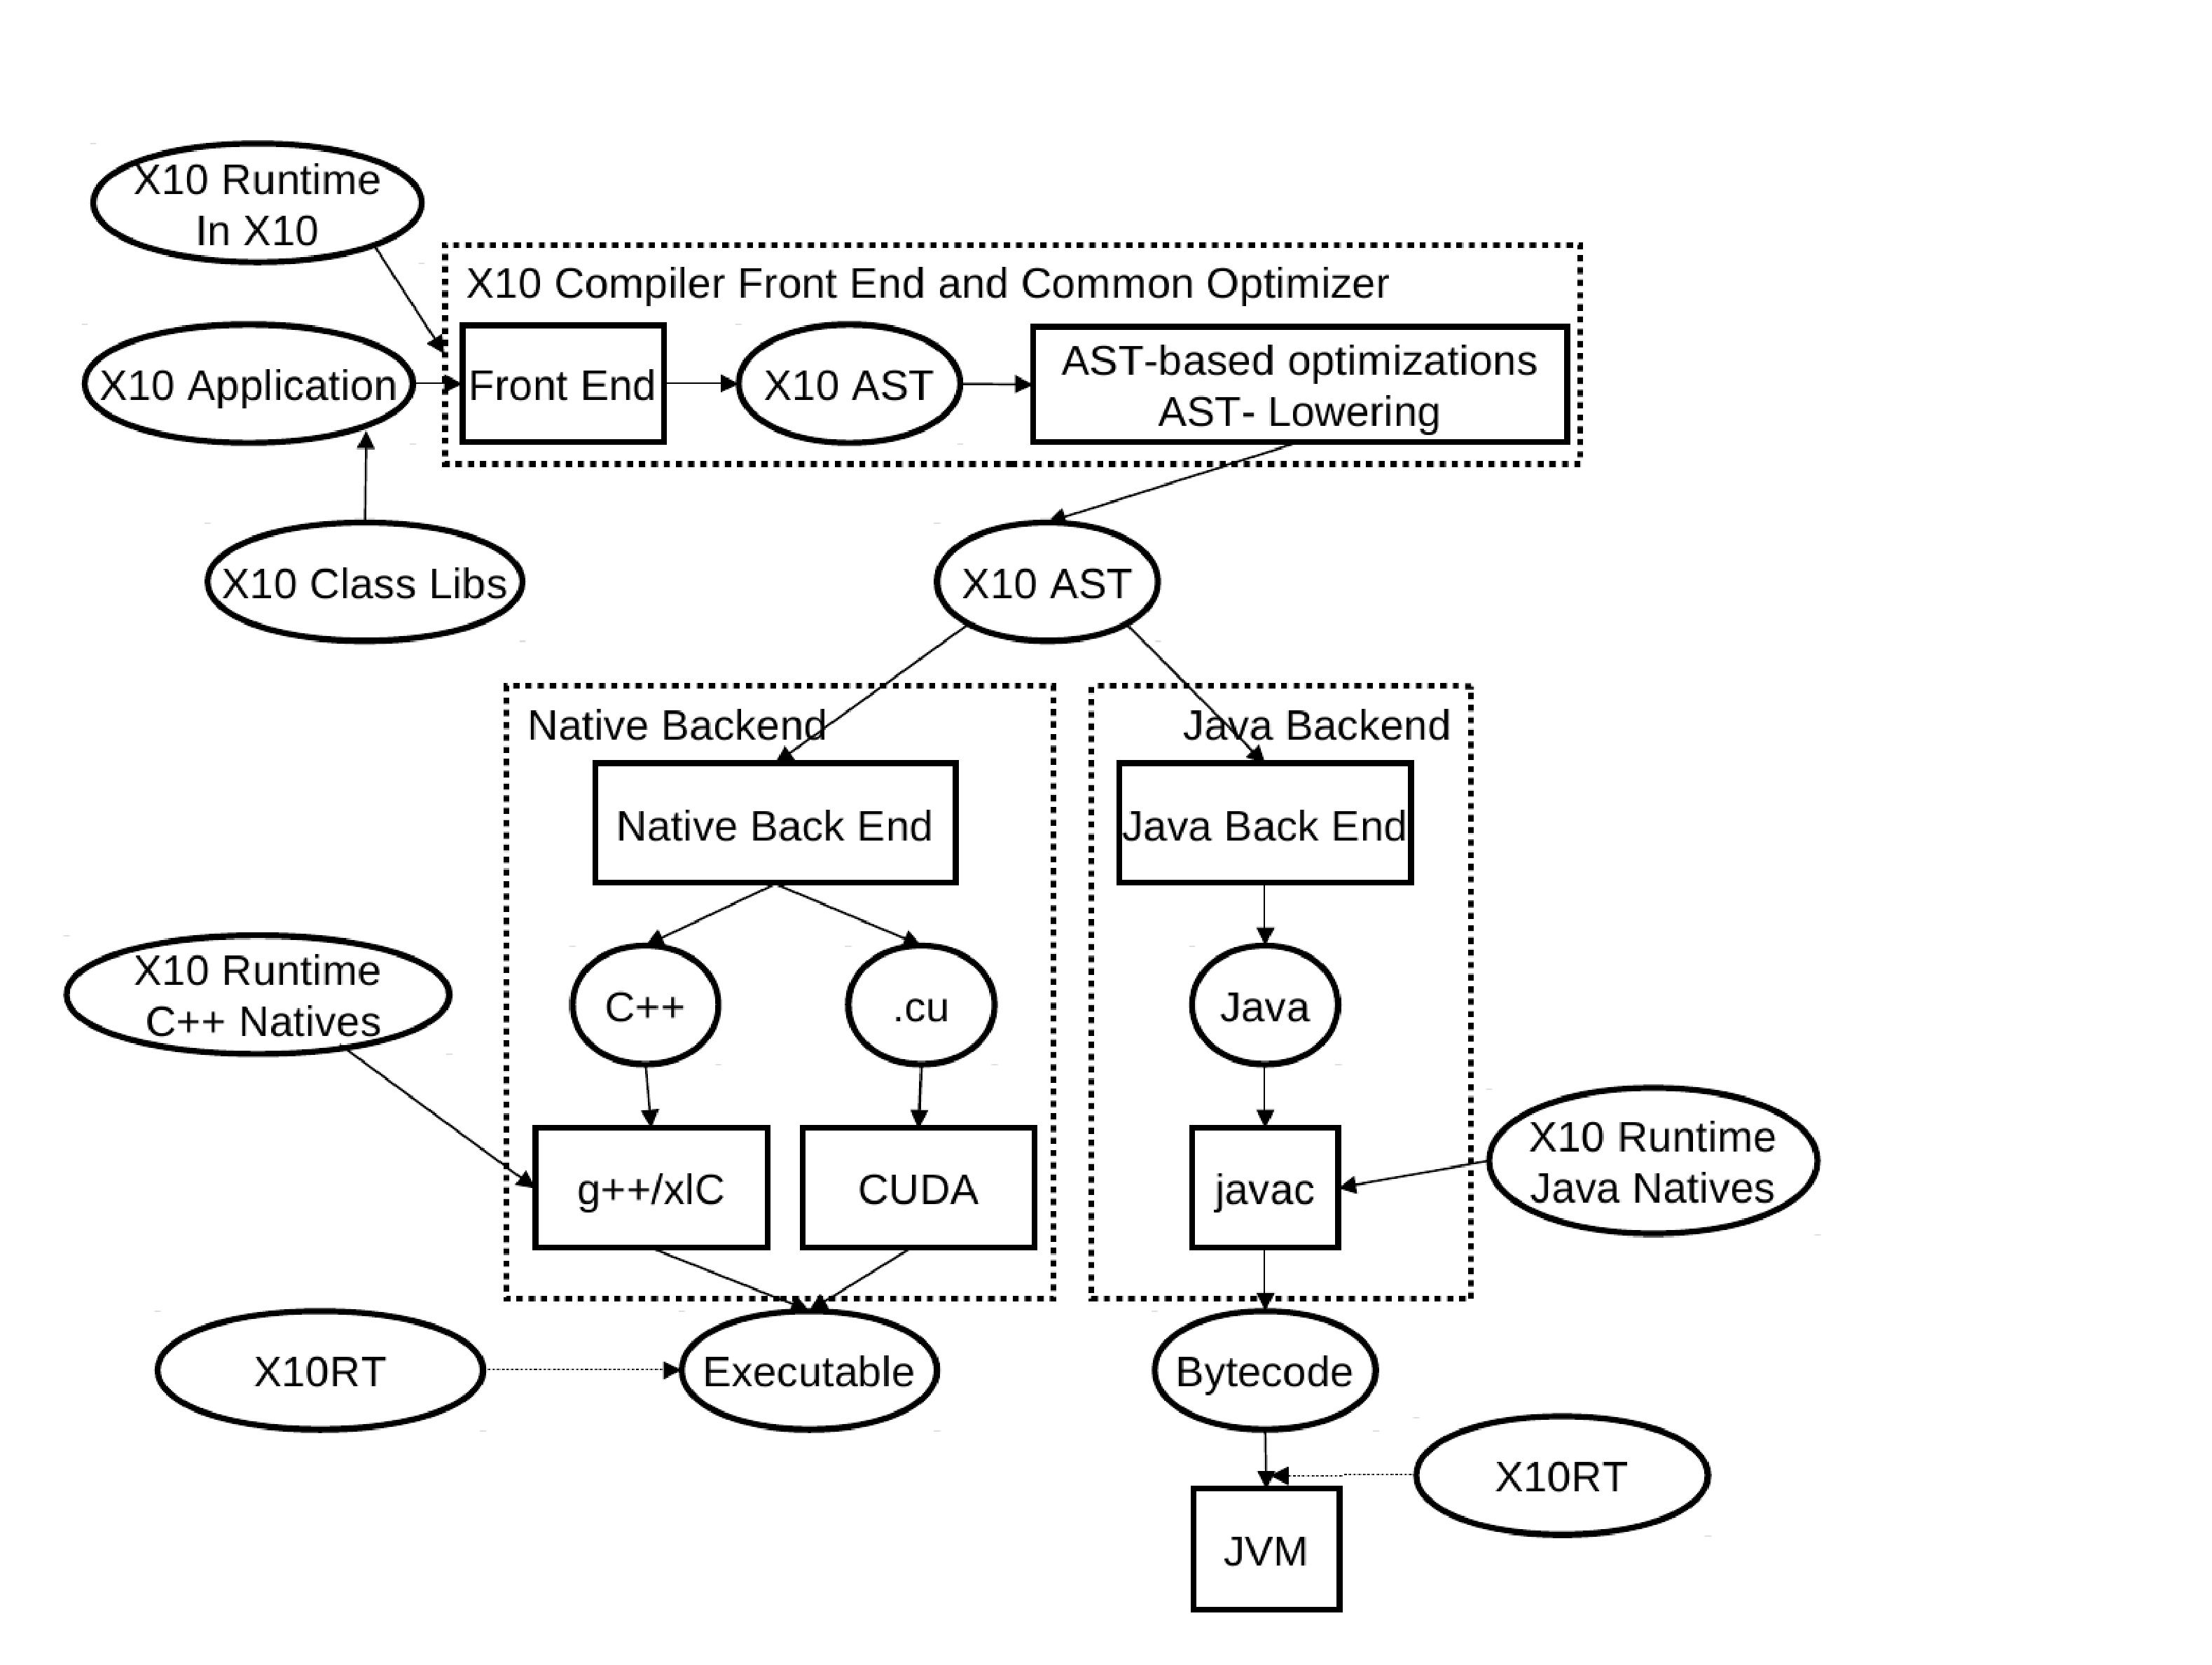
\includegraphics[width=0.8\textwidth]{Figures/x10compiler.eps}
    \caption{Architecture of the \xten compiler}
    \label{fig:x10compiler}
\end{figure}

\subsection{\xten Runtime}
Figure \ref{fig:x10runtime} shows the major components of the \xten runtime and
their relative hierarchy~\cite{x10intro}. 

The runtime bridges the gap between 
application program and
the low-level network transport system and the operating system. X10RT, which is
the lowest layer of the \xten runtime, provides abstraction and unification of
the functionalities provided by various network layers. 

The \xten Language
Native Runtime provides implementation of the sequential core of the language.
It is implemented in C++ for native \xten and Java for Managed \xten. 

XRX Runtime, the \xten runtime in \xten is the core of the \xten runtime system.
It provides implementation for the primitive \xten constructs for concurrency
and distribution (\texttt{async}, \texttt{finish}, \texttt{atomic} and
\texttt{at}). It is primarily written in \xten over a set of low-level APIs that
provide a platform-independent view of processes, threads, synchronization
mechanisms and inter-process communication. 

At the top of the \xten runtime system, is a set of core
class libraries that provide fundamental data types, basic collections, and key
APIs for concurrency and distribution.   

\begin{figure}[htbp]
    \centering
    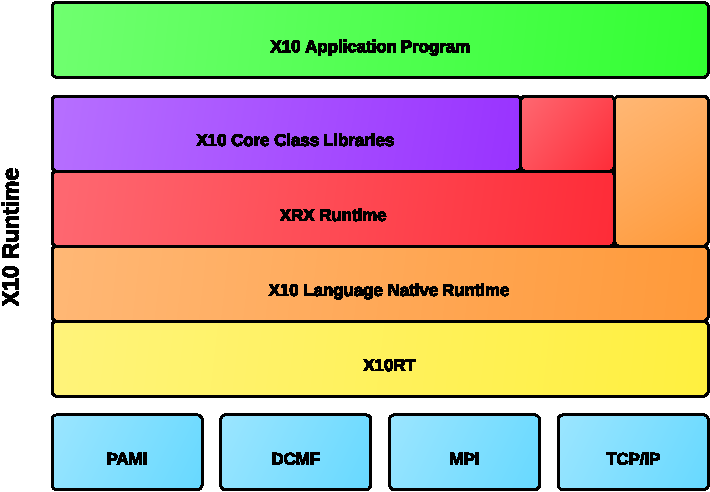
\includegraphics[width=0.77\textwidth]{Figures/x10rt.pdf}
    \caption{Architecture of the \xten runtime}
    \label{fig:x10runtime}
\end{figure}

%\section{Summary}
%
%In this chapter we have provided an overview of the key features of the \xten
%programming language. In the following chapters, specially chapters
%\chapref{chap:CodegenSeq} and \chapref{chap:Arrays}, we will discuss some of the
%features and constructs introduced here, in more depth. 
%
%We will also discuss key constructs and features of the \matlab
%programming language and contrast them with \xten, as we discuss \mixten's
%compilation strategies in the following chapters. For readers who are completely
%unfamiliar with \matlab or are interested in a quick overview, we suggest
%reading chapter 2 of \cite{AntonThesis}.
%   

%introduction to x10 and Matlab, highlighting the contrasts between two
%-intro to x10
%-intro to Matlab
%-Key differences between X10 and Matlab

\chapter{Background and High-level Design of \mixten} \label{chap:Design}
\section{Background}
% for the intro put listings into Matlab mode
\lstset{language=Matlab}

\mixten is implemented on top of several existing \matlab compiler tools.
The overall structure is given in \figref{Fig:Overview},  where the new
parts are indicated by the shaded boxes, and future work is indicated by
dashed boxes.     

\begin{figure}[htbp] 
\begin{center}
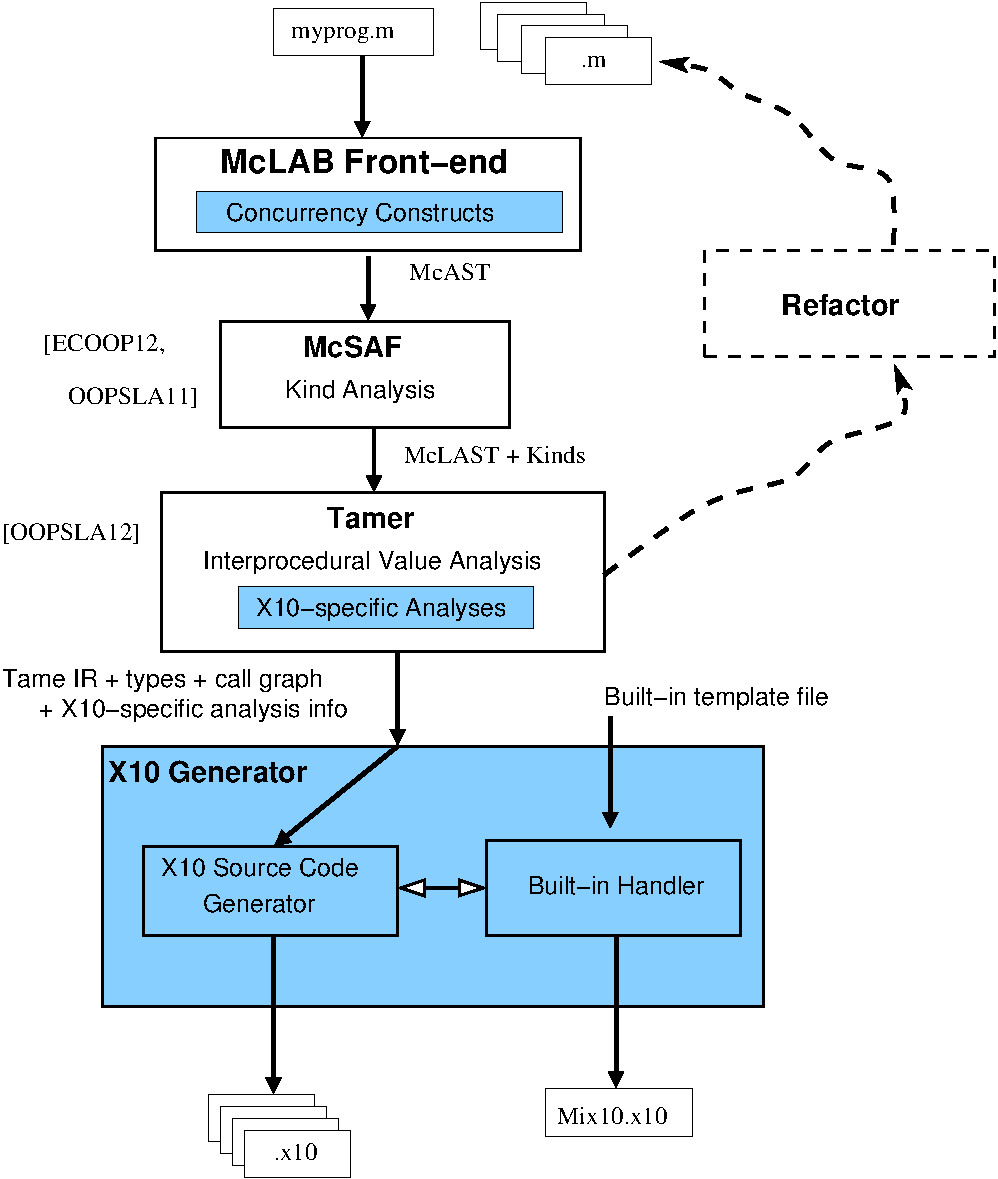
\includegraphics[width=3.2in]{Figures/overview.pdf} 
\caption {Overview of \mixten structure}\label{Fig:Overview}
\end{center}
\end{figure}

As illustrated at the top of the figure, a \matlab programmer only needs
to provide an entry-point \matlab function (called \texttt{myprog.m} in
this example),  plus a collection of other
\matlab functions and libraries (directories of functions)
which may be called, directly or indirectly, by the entry point.   The
programmer may also specify the types and/or shapes of the input
parameters to the entry-point function.   As shown at the bottom of the
figure, our \mixten compiler automatically produces a collection of
\xten output files which contain the generated \xten code for all
reachable \matlab functions, plus one \xten file called
\texttt{mix10.x10} which contains generated and specialized \xten code
for the required builtin \matlab functions.  Thus, from the \matlab
programmer's point of view,  the \mixten compiler is quite simple to
use.

\matlab is actually quite a complicated language to compile,  starting
with its rather unusual syntax,  which cannot be parsed with standard
LALR techniques.  There are several issues that must be dealt with
including distinguishing places where white space and new line characters have 
syntactic meaning, and filling in missing \lstinline!end! keywords,
which are sometimes optional.   The \mclab front-end
handles the parsing of \matlab through a two step process.  There is a
pre-processing step which translates \matlab programs to a cleaner
subset, called \textit{Natlab}, which has a grammar that can be
expressed cleanly for a LALR parser.    The \mclab front-end delivers a
high-level AST based on this cleaner grammar.  
\begin{comment}
 For the \mixten project
we have extended the front-end to handle \xten- inspired concurrency
constructs,  exposed in the \matlab program as extended comments.
\end{comment}

After parsing,  the next major phase of \mixten uses the \mcsaf
framework~\cite{McSAFecoop12,JesseThesis} to disambiguate identifiers
using \textit{kind analysis}~\cite{KindAnalysis}, which determines if an
identifier refers to a \textit{variable} or a \textit{named function}.
This is required because the syntax of \matlab does not distinguish
between variables and functions. For example, the expression
\lstinline!a(i)! could refer to four different computations,
\lstinline!a! could be an array or a function,  and \lstinline!i! could
refer to the builtin function for the imaginary value $i$,  or it could
refer to a variable \lstinline!i!.    The \mcsaf framework also
simplifies the AST, producing a lower-level AST which is more amenable
to subsequent analysis.

The next major phase is the Tamer~\cite{TamerPaper}, which is a key
component for any tool which statically compiles \matlab.  The Tamer
generates an even more defined AST called \textit{Tamer IR}, as well as
performing key interprocedural analyses to determine both the call graph
and an estimate of the base type and shape of each variable, at each
program point.   The call graph is needed to determine which files
(functions) need to be compiled,  and the type and shape information is
very important for generating reasonable code when the target language
is statically typed, as is the case for \xten.  

\begin{comment}
The Tamer may find dynamic \matlab features which cannot be statically
compiled, in which case it flags that feature as not tame,  and the
ultimate goal is to support a refactoring tool which would aid the
programmer to restructure their input \matlab program in order to
eliminate the wild feature.
\end{comment}

The Tamer also provides an extensible \textit{interprocedural value
analysis} and an interprocedural analysis framework that extends the
intraprocedural framework provided by \mcsaf.   Any static backend will
use the standard results of the Tamer,  but is also likely to implement
some target-language-specific analyses which estimate properties useful
for generating code in a specific target language. Currently, we have
implemented two analyses : (1) An analysis for determining if a \matlab
variable is \textit{real} or \textit{complex} to enable support for
complex numbers in \mixten and other \matlab compilers based on \mclab;
and (2) \emph{IntegerOkay} analysis to identify which variables can be
safely declared to be of an integer type (\texttt{Int} or \texttt{Long})
instead of the default type \texttt{Double}.  

For the purposes of \mixten, the output of the Tamer is a low-level,
well-structured AST, which along with key analysis information about the
call graph,  the types and shapes of variables, and X10-specific
information.   These Tamer outputs are provided to the code generator,
which generates \xten code, and which is the main focus of this thesis.

The \xten source code generator actually gets inputs from two places.  It uses
the Tamer IR it receives from the the Tamer to drive the code generation,  but
for expressions referring to built-in \matlab functions it interacts with the
\textit{Built-in Handler} which used the built-in template file we provide.  We
describe the functioning of the
built-in handler in \chapref{chap:Builtins}. 

\chapref{chap:Arrays} concentrates on generating efficient code for \matlab
arrays.  \chapref{chap:CodegenSeq} describes the code generation strategy for
the sequential core of \matlab, while \chapref{chap:CodegenCon} describes our
strategy to generate parallel \xten code for \matlab \texttt{parfor} construct,
and introducing \xten like concurrency constructs in \matlab. The focus of this
thesis is to address challenges in generating \emph{efficient} \xten code whose
performance is comparable to state-of-the-art tools that generate more
traditional imperative languages like C and Fortran.

\section{High-level Design of the \mixten Compiler}

The \mixten code generator is the key component which makes the
translation from the Tamer IR, which is based on \matlab programming
constructs and semantics,  to \xten.  The overall structure of the
\mixten code generator is given in \figref{Fig:x10}.

\begin{figure}[htbp] 
\begin{center}
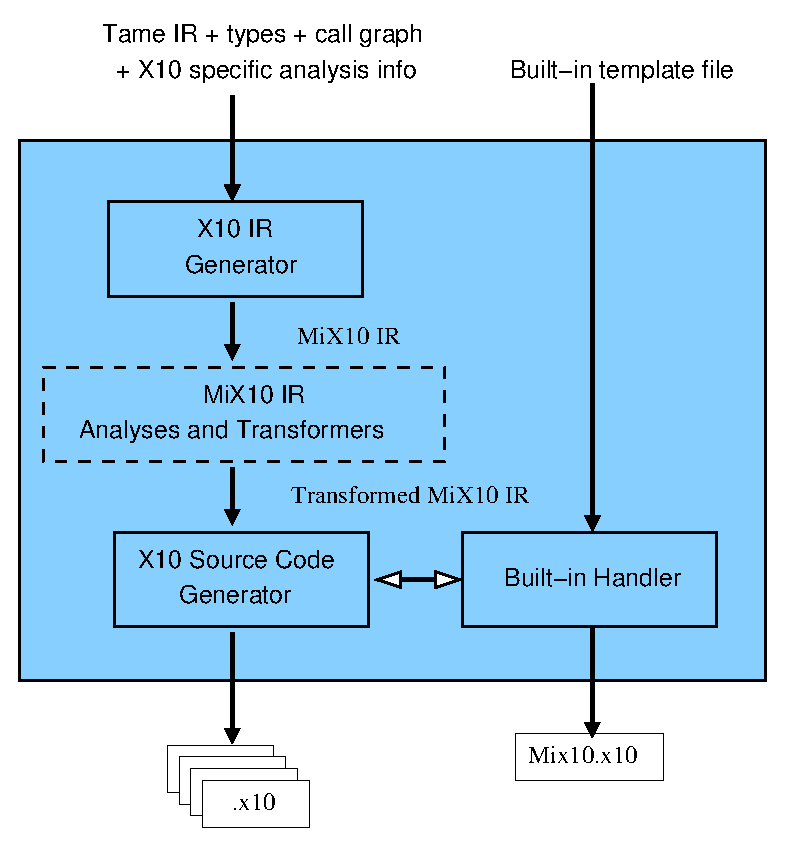
\includegraphics[width=3.2in]{Figures/x10.eps} 
\caption{Structure of the MiX10 code generator}\label{Fig:x10}
\end{center}
\end{figure}

 The input to to \mixten compiler is the call graph generated by Tamer and the
Tame IR annotated with the necessary analysis information like \emph{shape},
\emph{iscomplex}, and \emph{type} and \emph{IntegerOkay}.  Rather than do a
direct code generation to \xten source code, \mixten translates the Tamer IR to
\mixten IR, a general and extensible IR, designed by us, to represent \xten.
This translation is done by the \xten IR generator module of \mixten. Finally,
with the inputs from the builtin handler and the \xten IR generator (after the
\xten specific analyses and transformations have been done), the \xten source
code generator generates the resultatnt \xten source code.

\subsection{The \mixten Intermediate Representation}

The \mixten IR is a low-level, three address like intermediate representation
that is similar in design to the Tamer IR and abstracts the \xten constructs
while capturing the static information required to generate the \xten source
code.
We have implemented the IR using JastAdd~\cite{ekman04,jastaddurl}, which allows
us to easily add new AST nodes by simply extending the JastAdd
specification grammar.

There are three important reasons to use an IR, instead of directly generating the
\xten code: \begin{itemize} 

\item There are potentially two places that
optimizations and transformations may happen:  either at the Tamer IR level or
at the \mixten IR level.  It is our intent to put any analysis or transformation
that is not \xten-specific into the Tamer IR, so that other back-ends can
benefit from those improvements.   However, optimizations and  transformations
that are specific to \xten programming constructs (such as points and regions)
and semantics will need to be done on the \mixten IR. Although we currently do
not transform the \mixten IR very much, the ultimate goal is to support a
variety of analyses and transformations that can be used to: (1) produce more
efficient \xten code, and (2) produce more readable \xten code.  

\item There are \xten constructs that can be pretty
printed to be of different kinds, for example the \xten arrays, which can either
be simple arrays, region arrays or specialized region arrays, and \xten for loop
which can either be C-like for loop or an iterator over a \texttt{LongRange}
(used in generated code for \texttt{parfor} loop). It allows to abstract the
vital information for a construct while leaving the actual syntax to the source
code generator. This makes it easier to add \xten specific analyses and
transformations, and makes it easy to update the compiler whenever a new or
improved variation of a construct is added. 

\item \mixten IR can also be used as a convenient place to insert
instrumentation code for the generated \xten code.

\end{itemize}   

Appendix \ref{chap:irgrammar} provides the JastAdd implementation of the \mixten IR
grammar.

%As shown in \figref{Fig:x10}, the \xten source code generator actually
%gets inputs from two places.   It uses the \mixten IR to drive the code
%generation,  but for expressions referring to built-in \matlab functions
%it interacts with the \textit{Built-in Handler}.  In 
%\chapref{chap:Builtins}, we discuss this process in in more detail, and in
%the subsequent chapters,  \chapref{chap:CodegenSeq} and
%\chapref{chap:CodegenCon} we address the source code
%generation for the key \xten constructs.
%


%-Background
%-High level design of x10 generator
%-mix10 ir

\chapter{Techniques for Efficient Compilation of \matlab Arrays} 
\label{chap:Arrays}
\begin{comment}
-Key factors for efficient compilation of arrays
-how do we handle them
\end{comment}

Arrays are the core of the \matlab programming language. Every value in
\matlab is a \emph{Matrix} and has an associated array shape. Even
scalar values are represented as $1\times1$ arrays.  Most of the data
read and write operations involve accessing individual or a set of array
elements.  Given the central role of arrays in \matlab, it is of utmost
importance for our \mixten compiler to find effective and efficient
translations to \xten arrays. 

Given the shape information provided by the shape analysis engine~\cite{mc2for}
built into the \mclab analysis
framework~\cite{McSAFecoop12,JesseThesis,TamerPaper}, it was not hard to compile
\matlab arrays to \xten. However, to generate \xten code whose performance would
be competitive to the generated C code (via \matlab coder) and the generated
Fortran code (via the \mctwofor compiler), was not straightforward, and required
deeper understanding of the \xten array system and
careful handling of several features of the \matlab arrays.

\section{Simple Arrays or Region Arrays}\label{Sec:CompileArrays}

As described in Section \ref{subsec:ArrayDesc}, \xten provides two higher level
abstractions for arrays, simple arrays, a high performance but rigid
abstraction, and region arrays, a flexible abstraction but not as efficient as
the simple arrays. In order to achieve more efficiency, our strategy is to use
the simple arrays whenever possible, and to fall back to the region arrays when
necessary. Note that it is possible to force the \mixten compiler to use region
arrays via a switch, for experimentation purposes.

\subsection{Compilation to Simple Arrays}\label{sec:compsimple}
In dealing with the simple
rail-backed arrays, there were two important challenges.  First, we needed to
determine when it is safe to use the simple rail-backed arrays,  and second, we
needed  an implementation of simple rail-backed arrays that handles the
column-major, 1-indexing, and linearization operations required by \matlab.
     
\paragraph{When to use simple rail-backed arrays:} After the shape analysis of
the source \matlab program, if shapes of all the arrays in the program: (1) are
known statically, (2) are supported by the \xten implementation of simple arrays
and (3) the dimensionality of the shapes remain same at all points in the
program; then \mixten generates \xten code that uses simple arrays. 

\paragraph{Column-major indexing:} In order
to make \xten simple arrays more compatible with \matlab, we modified the
implementation of the \verb|Array_2| and \verb|Array_3| classes in
\verb|x10.array| package to use column-major ordering instead of the default
row-major ordering when linearizing multidimensional arrays to the backing
\verb|Rail| storage.\footnote{
\url{http://www.sable.mcgill.ca/mclab/mix10/x10_update/}} Since \matlab uses
column-major ordering to linearize arrays, this modification also makes it
trivial to support linear indexing operations in \matlab.  \footnote{
\url{http://www.mathworks.com/help/matlab/math/matrix-indexing.html}}
\matlab naturally supports linear indexing for individual element
access. More precisely, if the number of subscripts in an array access
is less than the number of dimensions of the array, the last subscript
is linearly indexed over the remaining number of dimensions in a
column-major fashion. Our modification to use column-major ordering for
the backing \verb|Rail| make it easier and more efficient to support
linear indexing by allowing direct access to the underlying \verb|Rail|
at the calculated linear offset.

Given that we can determine when it is safe to use the simple rail-backed
arrays,  and our improved \xten implementation of them,  we then designed the
appropriate translations from \matlab to \xten, for array construction, array
accesses for both individual elements and ranges. Given the number of dimensions
and the size of each dimension, it is easy to construct a simple array. For
example a two-dimensional array \verb|A| of type \verb|T| and shape $m\times n$
can be constructed using a statement like \texttt{val A:Array\_2[T] = new
Array\_2[T](m,n);}. Additional arguments can be passed to the constructor to
initialize the array. Another important thing to note is that \matlab allows the
use of keyword \verb|end| or an expression involving \verb|end| (like
\verb|end-1|) as a subscript. \verb|end|  denotes the highest index in that
dimension. If the highest index is not known the \verb|numElems_i| property of
the simple arrays is used to get the number of elements in the \verb|i|th
dimension of the array.  


\subsection{Compilation to Region Arrays}

With \matlab's dynamic nature and unconventional semantics, it is not
always possible to statically determine the shape of an arrays 
accurately.  Luckily, with some thought to a proper translation, \xten's
region arrays are flexible enough to support \matlab's ``wild" arrays.
Also, since \verb|Point| objects can be a set of arbitrary integers,
there is no restriction on the starting index of the arrays. Region
arrays can easily use one-based indexing. 

\paragraph{Array construction:}
Array construction for region arrays involves creating a region over a set of
points (or index objects) and assigning it to an array. Regions of arbitrary
ranks can be created dynamically.  
For example, consider the following \matlab code snippet:

\begin{minipage}{0.4\linewidth}
\begin{lstlisting}[language=Matlab,numbers=none]                                
function[x] = foo(a)                                                        
    t = bar(a);  
    x = t;
    ...	                                                                    
end      
\end{lstlisting}  
\end{minipage}
\hfill
\hspace{.5cm}
\hfill
\begin{minipage}{0.5\linewidth}
\begin{lstlisting}[language=Matlab,numbers=none]                                
function[y] = bar(a)
    if (a == 3)
        y = zeros(a,a+1,a+2,a+3);
    else
        y = zeros(a,a+1,a+2);
    end
end		                                                           
\end{lstlisting}  
\end{minipage}

\noindent
In this code, the number of dimensions of array \verb|t| and hence array
\verb|x| cannot be determined statically at compile-time. In such case, it is 
not possible to generate \xten code that uses simple arrays, however, it can 
still be compiled to the following \xten code for function \verb|foo()|.

\begin{minipage}{0.4\linewidth}
\begin{lstlisting}[language=X10,numbers=none]                                   
static def foo(a: Double){
  val t: Array[Double] = 
    new Array[Double](bar(a));
  val x: Array[Double] = 
    new Array[Double](t);
  ...
  return x;
}                         
\end{lstlisting}              
\end{minipage}
\hfill
\hspace{.3cm}
\hfill
\begin{minipage}{0.5\linewidth}
\begin{lstlisting}[language=X10,numbers=none]                                   
static def bar(a:Double){
  var y:Array[Double]=null;
  if (a == 3) {
    y = new Array[Double]
      (Mix10.zeros(a,a+1,a+2,a+3));
  }
  else {
    y = new Array[Double]
      (Mix10.zeros(a,a+1,a+2));
  }
  return y;
}		                        
\end{lstlisting}              
\end{minipage}

\noindent
In this generated \xten code, \verb|t| is an array of type \verb|Double|
which can be created by copying from another array returned by
\verb|bar(a)| without knowing the shape of the returned array. 

\paragraph{Array access:}
Subscripting operations to access individual elements are mapped to
\xten's region array subscripting operation. If the rank of array is 4
or less, it is subscripted directly by integers corresponding to
subscripts in \matlab otherwise we create a \verb|Point| object from
these integer values and use it to subscript the array. In case an
expression involving \verb|end| is used for indexing and the complete
shape information is not available, method \verb|max(Long i)|, provided
by the \verb|Region| class is used, allowing to determine the highest
index for a particular dimension at runtime.

\paragraph{Rank specialization:} Although region arrays can be used with
minimal compile-time information, providing additional static
information can improve performance of the resultant code by eliminating
run-time checks involving provided information. One of the key
specializations that we introduced with use of region arrays is to
specify the rank of an array in its declaration, whenever it is known
statically. For example if rank of an array \verb|A| of type \verb|T| is
known to be two, it can be declared as \verb|val A:Array[T](2);|.  This
specialization provided better performance compared to
unspecialized code as shown in section~\ref{sec:EvalArrays}.


\section{Handling the Colon Expression}

\matlab allows the use of an expression such as \verb|a:b| (or
\texttt{colon(a,b)}) to create a vector of integers 
\verb|[a, a+1,| \verb| a+2, ... b]|. In another form, an expression like 
\verb|a:i:b| can be used to
specify an integer interval of size \verb|i| between the elements of the
resulting vector. Use of a \verb|colon| expression for
array subscripting takes all the elements of the array for
which the subscript in a particular dimension is in the vector
created by the \verb|colon| expression in that
dimension.\footnote{Use of ':' in place of an index without lower and
upper bounds indicates the use of all the indices in that dimension.}
Consider the following \matlab code:

\begin{lstlisting}[language=Matlab,numbers=none]                                
function [x] = crazyArray(a)                                                    
    y = ones(3,4,5);                                                            
    x = y(1,2:3,:);                                                             
end                                                                             
\end{lstlisting}

\noindent
Here \verb|y| is a three-dimensional array of shape $3\times4\times5$ and
\verb|x| is a sub-array of \verb|y| of shape $1\times2\times5$. 
Such array accesses can be handled by simply calling the \verb|getSubArray[T]()|
that we have implemented in a Helper class provided with the generated code. 
The generated \xten code with simple array for this example is as follows:

\begin{lstlisting}[language=x10,numbers=none]                                
static def crazyArray (a: Double){
    val y: Array_3[Double] = new Array_3[Double](Mix10.ones(3, 4, 5));
    val mc_t0: Array_1[Double] = new Array_1[Double](Mix10.colon(2, 3));
    var x: Array_3[Double];
    x = new Array_3[Double](Helper.getSubArray(1, 1, mc_t0(0), mc_t0(1), 1, 5, y)) ;
    return x;
}
\end{lstlisting}

The colon operator can also be used on the left hand side for an array set
operation that updates multiple values of the array. For example, in the
\matlab statement \texttt{x(:,4) = y;}, all the values of the fourth column of
\verb|x| will be set to \verb|y| if \verb|y| is a scalar or to corresponding
values of \verb|y| if \verb|y| is a column vector with length equal to the size
of first dimension of \verb|x|. To handle this kind of operation we have
implemented another helper method, \texttt{setSubArray()}. This method takes as
input, the target array, the bounds on each dimension, and the source array.
\texttt{x(:,4) = y;} will be translated by \mixten to \texttt{x =
Helper.setSubArray(x, 1, x.numElems\_1, 4, 4, y);}

We have implemented overloaded versions of the \texttt{getSubArray()} and the
\texttt{setSubArray()} methods for arrays of different dimensions. For region
arrays, we provide the same methods that operate on region arrays in a different
version of the Helper class.  \mixten provides the correct version of the Helper
class, based on what kind of arrays are used.


\section{Array Growth} 

\matlab allows explicit array growth during runtime via the \texttt{horzcat()}
and the \texttt{vertcat()} builtin functions for array concatenation operations. 
In \mixten this feature is
supported for simple arrays as long as the array growth does not change the
number of dimensions of the array. For region arrays, this feature is supported
in full. For simple arrays, \xten allows a variable declared to be an array of
rank i, to hold any array value of the same rank. For example, consider the
following set of statements:
\begin{lstlisting}[language=x10,numbers=none]                                
//...
var x:Array_2[Long];
x = new Array_2(3,4,0);
y = new Array_2(3,5,0);
x=y;
//...
\end{lstlisting}
Here, \verb|x| is defined to be of type \texttt{Array\_2[Long]} and can hold
arrays of different sizes at different points in the program.

Region arrays, being more dynamic, also support array growth even if it changes
the rank of the array. For example, the following set of statements are valid in
an \xten program that uses region arrays:
\begin{lstlisting}[language=x10,numbers=none]                                
//...
var x:Array[Long];
x = new Array(Region.make(1..3,1..4),0);
y = new Array(Region.make(1..3,1..5,1..6),1);
x=y;
//...
\end{lstlisting}
Here \verb|x| is a 2-dimensional array and \verb|y| is a 3-dimensional array. 

\par
Section \ref{sec:EvalArrays} discusses the performance results obtained by
using
different kinds of arrays and provides a comparison of them, thus showing the
efficiency of our approach for compiling \matlab arrays to \xten.

%-Arrays

\chapter{Handling \matlab Builtins}
\label{chap:Builtins}
\matlab  builtin methods are the core of the language and one of the
features that make it popular among scientists. They provide a huge set
of commonly used numerical functions.  All the operators, including the
standard binary operators (\verb|+, -, *,/|), comparison operators
(\verb|<, >, <=, >=, ==|) and logical operators (\verb+&, &&, |, ||+)
are merely syntactic sugar for corresponding builtin methods that take
the operands as arguments. For example an expression like \verb|a+b| is
actually implemented as \verb|plus(a,b)|. An important thing to note is
that unlike most programming languages, all the \matlab builtin methods
by default operate on matrix values as a whole. For example \verb|a*b|
or \verb|mtimes(a,b)| actually performs matrix multiplication on matrix
values \verb|a| and \verb|b|.  However, most of the builtin methods also
accept one or more scalar, or more accurately, $1\times1$ matrix
arguments.
Builtin methods are overloaded to accept almost all possible shapes of
arguments. Thus \verb|mtimes(a,b)| can have both \verb|a| and \verb|b| as
matrix arguments (including $1\times1$ matrices) with number of columns in
\verb|a| equal to number of rows in \verb|b|, in which case the result
is a matrix multiplication of \verb|a| and \verb|b| or one of them can
be a $1\times1$ matrix and other can be a matrix of any size and the
result is a matrix containing each element of the non-scalar argument
times the scalar argument.  Wherever possible, \matlab builtins also
support complex numerical values.  \xten on the other hand, like most of
the programming languages operates on scalar values by default.
 
Due to the fact that \xten is still new and evolving, it has a very
limited set of libraries, specially to support a large subset of
available \matlab builtin methods. The \xten Global Matrix Library (GML)
supports double-precision matrix operations however it is still not as
extensive as \matlab's set of operations and it poses some restrictions:

\begin{enumerate}

\item It works on values of type \verb|Matrix| instead of \xten type
\verb|Array| which means it needs explicit conversion of \verb|Array|
values to \verb|Matrix| values before performing a matrix operation and
and then a conversion of the results back to \verb|Array| type. This
conversion may be  a large overhead, especially for small data sizes.

\item GML is limited to Matrix values of two dimensions and containing
elements of type \verb|Double|, whereas many \matlab builtin methods
support values of greater number of dimensions.

\item GML currently does not support complex numerical values whereas
\matlab naturally supports them.

\item Currently GML requires a separate installation and configuration which
is non-trivial specially for scientists who need something that works
out of the box.

%\item TODO:verify if GML provides overloaded methods for scalars

\end{enumerate}

Due to above restrictions, \xten Global Matrix Library is useful in some
situations, for example when there is a matrix multiplication of a very
large data size, but cannot be used or is not a good choice for a large
number of operations.

For a language with open-sourced libraries, it would be possible to actually
compile the library methods to \xten.  However,  many \matlab libraries 
are closed source and thus it is not possible to translate them to \xten.

\subsection{ The \mixten Builtin Support Framework}

We decided to write our own \xten implementations of the commonly used
\matlab builtin methods. Currently we have implemented
only those methods that are used in our benchmarks. In this thesis, we
concentrate on how these methods are included in the generated \xten
code with minimal loss of readability and performance rather than the
actual implementation.

The code below shows the \xten code for the \matlab builtin method
\verb|plus(a,b)| involving 2-dimensional simple arrays.

\noindent
\begin{lstlisting}[language=X10,numbers=none]
public static def 
  plus(a: Array_2[Double], b:Array_2[Double]){
		val x = new Array_2[Double](a.numElems_1, a.numElems_2);
		for (p in a.indices()){
			x(p) = a(p)+ b(p);
		}
  	return x;
}
	
public static def plus(a:Double, b:Array_2[Double]){
	val x = new Array_2[Double](b.numElems_1, b.numElems_2);
	for (p in b.indices()){
		x(p) = a+ b(p);
	}
	return x;
}
	
public static def plus(a:Array_2[Double], b:Double){
	val x = new Array_2[Double](a.numElems_1, a.numElems_2);
	for (p in a.indices()){
		x(p) = a(p)+ b;
	}
	return x;
}
	
public static def plus(a:Double, b:Double){
	val x: Double;
	x = a+b;
	return x;
}
\end{lstlisting}

This \xten code contains four overloaded versions (and it still does not
contain methods to support complex values, variables of types other than Double,
simple arrays of other dimensions, and region arrays) based 
on whether the arguments are scalar or \texttt{Array\_2} and their relative position
in the list of arguments. 

Including all the overloaded versions and versions specialized for arrays of
different dimensions or region arrays, in the generated \xten code would result
in lot of lookup overhead, would require producing redundant code (versions
of methods with arguments of similar shape but different types will have the
same algorithm) and would generate large code with less readability. Instead we
designed a specialization technique that selects the appropriate versions of
only the methods used in the source \matlab program. Note that the use of
generic types to handle arguments of different types is not always a good idea,
since several builtin implementations involve calls to \xten library functions
which are not defined on generic types. For example, functions in the
\texttt{x10.lang.Math} librarry like \texttt{floor(Double a)},
\texttt{max(Double a, Double b)}, etc. do not take generic type arguments. 

After studying numerous builtin methods we categorized them into the
following five categories:

\begin{description}
\item[Type 1:] All the parameters are scalar values or no parameters.
\item[Type 2:] All the parameters are arrays.
\item[Type 3:] First parameter is scalar, rest of the parameters are arrays.
\item[Type 4:] Last parameter is scalar, rest of the parameters are arrays.
\item[Type 5:] Any other type(Default).
\end{description}

Each of these categories, except \emph{Type 5}, uses similar code template for
different types of values. Note that due to the three address code-like
structure of Tame IR, any call to a builtin almost always contains zero, one or
two arguments. For builtin calls like \texttt{horzcat} and \texttt{vertcat}
which may contain variable number of arguments, \mixten packs all the arguments
in a \texttt{Rail} and passes a single argument of type \texttt{Rail}.
Accordingly, these builtins are implemented in \emph{Type 2} category and receive a
single argument of type \texttt{Rail}.

We build an XML file that contains the method bodies for each category for
every builtin method (that we support). The XML also contains specialized
implementations of every builtin for different kinds of arrays.  We implement
the following strategy to select and generate the correct and required methods.
First, we make a pass through the AST to make a list of all the builtin methods
used in the source \matlab program. Next, we parse the XML file once and read
in the \xten code templates for all the categories of the builtin methods
collected in the first step. Next, whenever a call to a builtin method is made,
based on the results of the value analysis we: (1) Identify the required
specialization for the method (simple array or region array); and (2) generate
the correct method header and select the corresponding builtin template in the
required specialization for that method.  The generated methods are finally
written to a \xten class file named \verb|Mix10.x10|. In the code generated for
actual \matlab program, the call to a builtin method is simply replaced by a
call to the corresponding method in the Mix10 class. For example, \matlab
expression \verb|plus(a,b)| is translated to \xten expression
\verb|Mix10.plus(a,b)|. Appendix \ref{chap:Builtinxml} demonstrates the
structure of the builtin XML with an example implementation of the builtin
\texttt{plus}. 

Using the above approach not only improves the readability of the generated
code, but it also allows for future extensibility, better maintenance and more
specialization. Specializations that we plan to add in future are: (1) the
ability to use the Global Matrix Library for the available methods in it and
whenever the data size is large enough; and (2) concurrent versions of the
relevant builtins to support the execution of vector instructions in parallel
fashion, as
described in section \ref{sec:parvec}. We also encourage advanced users to
mdoify the generated \texttt{Mix10.x10} file to enhance or add builtin
implementations for higher performance of the generated code. 



\chapter{Code Generation for the Sequential Core} \label{chap:CodegenSeq}
\matlab is a programming language designed specifically for numerical
computations. Every value is a \emph{Matrix} and has an associated array
shape.  Even scalar values are $1\times1$ matrices. Vectors are
$1\times n$ or $n \times 1$ matrices. All the values are by default of
type \verb+double+.  \matlab naturally supports imaginary components for
all numerical values and almost all operators and library functions
support complex inputs. In the rest of this chapter we describe some of
the key features of \matlab that demonstrate what makes \matlab 
different and challenging to compile statically and techniques used by
\mixten to translate these ``wild" features to \xten. We provide necessary
details on the various \matlab constructs as we discuss them, however for the
readers who are totally unfamiliar with \matlab, we suggest reading chapter 2 of
the M.Sc. thesis on the Tamer framework~\cite{adubra12}. 

\section{Methods}

A function definition in \matlab takes one or more input arguments and
returns one or more values. A typical \matlab function looks as follows:

%\lstset{tabsize=2}
\begin{lstlisting}[language=Matlab,numbers=none]
function[x,y] = foo(a,b)
    x = a+3;
    y = b-3;
end
\end{lstlisting}

This function has two input arguments \verb|a| and \verb|b| that
can be of any type and any shape and returns two values \verb|x| and
\verb|y| of the same shape as \verb|a| and \verb|b| respectively and of
types determined by \matlab's type conversion rules. The Tamer IR
provides a list of input arguments and a list of return values for a
function. The interprocedural value analysis identifies the types,
shapes and whether they are complex numerical values for all the
arguments and the return values.

\matlab functions are mapped to \xten methods. If it is the entry
function, the type of the input argument is specified by the user (Tame
IR requires to have an entry function or a driver function with one
argument. This function may call other functions with any number of
input arguments). For other functions the parameter types are computed
by the value analysis performed by the Tamer on the Tame IR. The type
information computed includes the type of the value, its shape and
whether it is a complex value. Other statements in the function block
are processed recursively and corresponding nodes are created in the
\xten IR. Finally, if there are any return values, as determined by the
Tame IR, a return statement is inserted in the \xten IR at the end of
the method. If the function returns only one value, say \verb|x| then
the inserted statement is simply \verb|return x;| but if the function
returns more than one values (which is quite common in \matlab) then we
return a \texttt{Rail} of type \verb|Any| whose elements are the
values that are returned. So, for the above example the return statement
is \verb|return [x as Any, y as Any];|. Note that the use of short syntactic form
for \texttt{Rail} construction improves the readability of the
generated code. Below is the generated code for the simple example
above.

\begin{lstlisting}[language=X10,numbers=none]
static def foo(a: Double, b: Double){
    var mc_t0: Double = 3.3;
    var x: Double = Mix10.plus(a, mc_t0);
    var mc_t1: Double = 3.2;
    var y: Double = Mix10.minus(b, mc_t1);
    return [x as Any, y as Any];
}
\end{lstlisting}

Also note that the variables \verb|mc_t0| and \verb|mc_t1| are introduced by
Tamer in the Tame IR. 


\section{Types, Assignments and Declarations}

\matlab provides following basic types:
\begin{itemize}
\item \verb|double, single|: floating point values
\item \verb|uint8, uint16, uint32, uint64|: unsigned integer values 
\item \verb|int8, int16, in32, int64|:	integer values
\item \verb|logical|: boolean values
\item \verb|char|: character values (strings are vectors of \verb|char|)
\end{itemize}

These basic types are naturally mapped to \xten base types as follows.  Floating
point values are mapped to \verb|Double| and \verb|Float| respectively, unsigned
integers are mapped to \verb|UByte, UShort, UInt| and \verb|ULong|, integer
values are mapped to \verb|Byte, Short, Int| and \verb|Long|, \verb|logical| is
mapped to \verb|Boolean| and \verb|char| is mapped to \verb|Char| (vector of
chars is mapped to \verb|String| type). If the shape of an identifier of type
\verb|T| is greater than $1\times1$ it is mapped to \verb|Array[T]|.  The type
conversion rules are quite different from standard languages.  For example, an
operation involving a \verb|double| and an \verb|int32| results in a value of
type \verb|int32|.\footnote{The type rules are explained in detail in the Tamer
documents, \url{www.sable.mcgill.ca/mclab/tamer.html.}}  \mixten inserts an
explicit typecast wherever required.
  
All the \matlab operators are designed to work on matrix values and are provided
as syntactic sugar to the corresponding builtin methods that take operands as
arguments.  Operators are overloaded to support different semantics for
$1\times1$ matrices (scalar values). \matlab provides two types of operators -
\emph{matrix operators} and \emph{array operators}. Matrix operators work on
whole matrix values.  These include matrix multiplication (\verb+*+) and matrix
division (\verb+\+, \verb+/+). Array operators always operate in an element-wise
manner. For example array multiply operator \verb+.*+ performs element-wise
multiplication. As described in \chapref{chap:Builtins}, \mixten implements all
operators as builtins.

\matlab is a dynamically typed language which means that variables need
not be declared and take up any value that they are assigned to. \xten
however, is statically typed and requires variables to be declared before
being assigned to. \mixten maintains a list of all the declared
variables. It starts with an empty list. Whenever an identifier appears
in an assignment statement on LHS, if it is not already present in the
list, a declaration statement is added to the \xten IR and the variable
(with its associated type and value information) is added to the list, followed
by an assignment statement corresponding to the statement in \matlab.
If the identifier is already present in the list, the assignment statement is
added to the \xten IR and the associated type and value information is
updated. In case the \matlab assignment statement is inside a loop and
needs a declaration, the declaration statement (without any assignment)
is added to the method block outside any loop or conditional scope and
the assignment statement is added in the scope where it is present in
\matlab code. If the identifier on LHS is an array, then the declaration
creates a new array with the shape corresponding to the shape of the
RHS array. For example a \matlab statement like \verb|a=b;| where shape of
\verb|a| is, say, $3\times3$ and type is \verb|double| will be
translated to \verb|a:Array_2[Double]=new Array_2[Double](b);| for simple arrays
and \verb|a:Array[Double]=new Array[Double](b);| for region arrays
(outside the scope of any loops or conditionals). 
 
\section{Loops}

Loops in \matlab are fairly intuitive except for one semantic difference
from most of the languages. In a \verb|for| loop if the loop index
variable is redefined inside the body of the loop, then its new value is
persistent only in a particular iteration and does not affect the number
of loop iterations. For example, consider the following listing.

\begin{lstlisting}[language=Matlab,numbers=none]
function [x] =  forTest1(a)
    for i = (1:10)
        i=3;
        a=a+i;
    end
    x=a;
end
\end{lstlisting}

\noindent 
Note that inside every iteration, the value of loop index
variable \verb|i| is 3 but the loop still terminates after ten
iterations. The above code would be translated to the following \xten
code:

\begin{lstlisting}[language=X10,numbers=none]
static def forTest1 (a: Double)
{
  //Note that in the actual generated code
  //the name of the temporary variable introduced by MiX10
  //is mangled to ensure that there is no 
  //conflict with any other variable name. 
  
  var mc_t0: Long = 1;
  var mc_t1: Long = 10;
  var i_x10: Long;
  var b: Double;
  var i: Long;
  for (i_x10 = mc_t0; (i_x10 <= mc_t1); i_x10 = (i_x10 + 1))
      {   
           i = i_x10;
           i = 3 ;
           b = Mix10.plus(a, i) ;
      }
  var x: Double = a;
  return x;
}
\end{lstlisting}

To handle this somewhat different semantics we introduce a new loop
index variable and assign it to the original loop index variable at the
beginning of the loop body. The rest of the loop body is translated by
standard rules.  Note that the new loop index variable is
introduced only if the actual loop index variable is redefined inside
the loop body. 

\section{Conditionals}

In \matlab conditionals are expressed using the if-elseif-else construct
and do not have any wild semantics. \matlab also allows switch
statements which are converted to equivalent if-else statements by the
Tamer. It also recursively converts a statement like 
\texttt{if (B1) S1 elseif (B2) S2 else S3} to a series of if-else clauses like 
\texttt{if (B1) S1 else\{ if(B2) S2 else S3\}}. This if-else construct is 
intuitively mapped to the if-else construct in \xten. 

%\section{Colon operator} 

%\section{Array access and Colon operator}
%
%Arrays (or matrices) are the core of \matlab and most of the data read and
%write operations involve accessing one or a set of elements of an array. There
%are two basic ways of accessing elements of an array, as described below.
%
%
%\paragraph{Accessing individual elements:}  
%This type of access is similar to that in
%C or Java where an array element is accessed given its location index along
%each dimension of the array. \matlab naturally supports linear
%indexing\footnote{
%\url{http://www.mathworks.com/help/matlab/math/matrix-indexing.html}}
%More precisely, if the
%number of subscripts in an array access is less than the number of dimensions
%of the array, the last subscript is linearly indexed over the remaining number
%of dimensions in a column-major fashion. (Support for linear indexing in
%\mixten is currently a work in progress). Note that array indexing in
%\matlab starts from 1. \matlab allows the use of keyword \verb|end| or an
%expression involving \verb|end| (like \verb|end-1|) as a subscript. \verb|end|
%denotes the highest index in that dimension. 
%
%This subscripting operation to access individual elements is mapped to
%\xten array subscripting operation. If the rank of array is 4 or less,
%it is subscripted directly by integers corresponding to subscripts in
%\matlab otherwise we create a \verb|point| object from these integer
%values and use it to subscript the array. In case \verb|end| is used,
%if we have complete shape information we easily know the highest index
%for a particular dimension, otherwise if shape information cannot be
%determined at compile time we use the \verb|max(Int i)| method provided
%by the \verb|Region| class of \xten. Thus an array access such as 
%\verb|a(i,end)| is translated to \verb|a(i as Int, a.region.max(1))|.
%Whenever an identifier of type \verb|Double| (default in \matlab) is
%used as a subscript, we need to explicitly cast it to \verb|Int|.  
%
%\paragraph{Accessing a set of elements:}  \matlab supports accessed and
%operations on a set of elements as a whole. To achieve this \matlab
%allows the use of an expression involving \verb|colon| operator in place
%of an integer subscript.  An expression such as \verb|a:b| (or
%\verb|colon(a,b)|) creates a vector of 
%integers \verb|[a, a+1, a+2, ...b]|.\footnote{See
%\url{http://www.mathworks.com/help/matlab/ref/colon.html.}} In a second
%form, an interval size can also be provided. For example \verb|a:i:b|
%with interval size \verb|i| creates a vector \verb|[a, a+i, a+2i, ...k]| 
%where \verb|k| is the greatest integer such that \verb|b-k<i|. Use
%of a \verb|colon| expression for array subscripting takes all the
%elements of the array for which the subscript in a particular dimension
%is in the vector created by the \verb|colon| expression in that
%dimension.  For array subscripting we can also use "\verb|:|" without
%specifying the lower and the upper limit. In this case elements for all
%the indices in that particular dimension are accessed. 
%
%Consider the \matlab code below:
%
%\begin{lstlisting}[language=Matlab,numbers=none]
%function [x] = crazyArray(a)
%    y = ones(3,4,5);
%    x = y(1,2:3,:);
%end 
%\end{lstlisting}
%
%In this code \verb|y| is a 3-dimensional array of shape $3\times4\times5$.
%\verb|x| is an array created by copying the elements of \verb|y| at 
%\verb|(1,2,1), (1,2,2), |\\*
%\verb|... (1,2,5), (1,3,1), (1,3,2),| 
%\verb|... and (1,3,5)|. However \verb|y| itself is of shape $1\times2\times5$ and is indexed normally.
%This code is translated into the following \xten code.\footnote{Note
%that we are currently implementing aggregation transformations which
%will aggregate expressions, including folding constants into
%expressions.}
%
%\begin{lstlisting}[language=X10,numbers=none]
%public static def crazyArray(a: Double){
%    var mc_t1: Double = 3;
%    var mc_t2: Double = 4;
%    var mc_t3: Double = 5;
%    val y: Array[Double] = 
%             new Array[Double]( Mix10.ones(mc_t1, mc_t2, mc_t3));
%    var mc_t4: Double = 2;
%    var mc_t5: Double = 3;
%    val mc_t0: Array[Double] = 
%             new Array[Double]( Mix10.colon(mc_t4, mc_t5));
%    var mc_t6: Double = 1;
%    val x: Array[Double];
%    val mix10_pt_y: Point;
%    mix10_pt_y = Point.make(1-(mc_t6 as Int), 
%                  1-(mc_t0(mc_t0.region.min(0)) as Int), 0);
%    x = new Array[Double]((1..1)*
%         ((mc_t0.region.min(0)) as Int..
%          (mc_t0.region.max(0)) as Int)*
%          ((y.region.min(2))..y.region.max(2)),
%           (p:Point(3))=>y(p.operator-(mix10_pt_y))); 
%}
%\end{lstlisting}
%
%Our current shape analysis engine does not compute the shape of arrays
%involving \verb|colon| operator but we can use the \\ \verb|Region.min(Int i)| 
%and \verb|Region.max(Int i)| methods to compute the correct values
%at run time. In the above example, we first create a new \verb|Point|
%object that serves as an offset to get the elements at the correct
%position of the array accessed. Then we create the new array with region
%derived from the resultant vector from the \verb|colon| operator for
%second dimension and from the third dimension of the source array
%\verb|y|. Thus the resultant array \verb|x| has the region
%\verb|1..1*1..2*1..5|. Note that \mixten creates arrays with
%starting index 1 to maintain readability of the generated code for
%\matlab users. This is easy due to region-based arrays in \xten.
%Providing support for \verb|colon| operator in array access on LHS of an
%assignment statement and support for \verb|colon| operator with
%specified interval value is currently a work in progress.
   
\section{Function Calls}

Function calls in \matlab are similar to other programming languages if
the called function returns nothing or returns only one value. However,
\matlab allows a function to return multiple values.
Whenever a call is made to such a function, returned values are received
in a list in the order specified by function definition. For example in
the statement \verb|[x,n] = bubble(a);| a call is made to the function
\verb|bubble| which returns two values that are read into \verb|x| and
\verb|n| respectively. This statement is compiled to following code in
\xten.

\begin{lstlisting}[language=X10,numbers=none]
  
  //Note that in the actual generated code
  //the name of the temporary variable introduced by MiX10
  //is mangled to ensure that there is no 
  //conflict with any other variable name. 
  
   var x: Double;
   var n: Double;
   val _x_n: Rail[Any];
   _x_n = bubble(A) ;
   x = _x_n(0) as Double ;
   n = _x_n(1) as Double ;
\end{lstlisting}

The key idea here is to create a \texttt{Rail} of type \verb|Any| and read the
returned value. Remember that \mixten packs the multiple return values
of a method in a Rail of type \verb|Any| and returns it.  Individual
elements of the list simply read the values from this array. If the
function call is inside a loop, all the declarations are moved out of
the loop and only assignments are inside the loop. 

\section{Cell Arrays}

Cell arrays in \matlab are arrays of data containers called cells and
each cell can contain data of any type. For example \texttt{fooCell =
\{'x',10,'I like',ones(3,3)\};} creates a cell array containing values
of type char, double, char array and a double array. To convert to
\xten, the elements of the cell array are packed into a \texttt{rail} of
type \verb|Any|. While accessing an element it is type cast into its
original type.  Consider the following \matlab listing:
  
\begin{lstlisting}[language=Matlab,numbers=none]
function [x] =  cellTest(a)
	m = ones(2,3);
	n = [4,5];
	myCell = {m, n*100};
	x = myCell{1,2};
end
\end{lstlisting}

It creates a cell array containing two arrays. It is translated to the below
\xten code:

\begin{lstlisting}[language=X10,numbers=none]
static def cellTest (a: Double)
	{ 
    //Note that for the purpose of demonstration,
    //this example uses region arrays and
    //does not use IntegerOkay analysis.
		
    var mc_t2: Double = 2;
		var mc_t3: Double = 3;
		var m: Array[Double] = new Array[Double](Mix10.ones(mc_t2, mc_t3));
		var mc_t5: Double = 4;
		var mc_t6: Double = 5;
		var n: Array[Double] = new Array[Double](Mix10.horzcat(mc_t5, mc_t6));
		var mc_t0: Array[Double] = new Array[Double](m);
		var mc_t7: Double = 100;
		var mc_t1: Array[Double] = new Array[Double](Mix10.mtimes(n, mc_t7));
		var myCell: Rail[Any] = [mc_t0 as Any ,mc_t1 as Any];
		var mc_t9: Double = 1;
		var mc_t10: Double = 2;
		var x: Array[Double];
		x = myCell(mc_t9 as Long -1, mc_t10 as Long -1) as Array[Double];
		return x;
	}
\end{lstlisting}

%-Handling various matlab constructs

\chapter{Code Generation for Concurrency in \matlab} \label{chap:CodegenCon}
\matlab programmers often recognize the parallel nature of computations involved
in their programs but cannot express it due to the lack of fine-grained
concurrency controls in \matlab. Some concurrency can be achieved using controls
like \verb|parfor| and other tools in Mathwork's parallel computing toolbox, but
this has several drawbacks:  (1) the parallel toolbox is limited in terms of
scaling (\matlab currently supports only up to 12 workers \emph{processes} to
execute applications on a multicore processor~\cite{pct}); (2) the parallel
toolbox must be purchased separately, so not even all licensed \matlab users
will have it available; and (3) \matlab's concurrency is often slower compared
to \xten's concurrency controls (as shown in section~\ref{sec:parfor_results}).
Vectorization
\footnote{\url{http://www.mathworks.com/help/matlab/matlab_prog/vectorization.html}}
is a technique to convert loop-based scalar operations to vector operations, for
which \matlab is optimized.   So, another way of exposing parallelism in \matlab
is to optimize these instructions to perform the computations concurrently on
the elements of the vector.

\secref{sec:XX} gives an introduction to the concurrency controls in \xten.
Readers not familiar with \xten may find it useful to read it before continuing
with this chapter.



\section{Code Generation for the \matlab \texttt{parfor} Loop Construct}

The \matlab \texttt{parfor} construct is an important feature in \matlab and is
provided by the Mathworks' parallel computing toolbox~\cite{pct}. It allows the
for loop iterations in the \matlab programs to be executed in parallel, whenever
safely possible, thus greatly enhancing the performance of the for loop
execution. Other static \matlab compilers like \matlab coder and \mctwofor do
not support the \texttt{parfor} loop due to the lack of builtin concurrency
features in their target languages, C and Fortran. However, \xten, being a
parallel programming language, naturally provides concurrency control features.
The \mixten compiler supports parallel code generation for the \matlab
\texttt{parfor} construct and provides significantly better performance compared
to \matlab code with \texttt{parfor}, and also the sequential version of the
\xten code generated for the same program.   

The  \verb|parfor| (or parallel
for loop) is a key parallelization control provided by the
\matlab parallel computing toolbox that can be used to execute each
iteration of the for loop in parallel with each other. The challenge was
to implement it with \xten's concurrency controls while maintaining its
complex semantics and aiming for better performance than provided by the
parallel computing toolbox. 
There are three important semantic characteristics of \matlab's
\verb|parfor| loop: 
\begin{enumerate}
\item the scope of variables inside a \verb|parfor|
loop, including the loop index variable, is limited to each iteration.

\item if a variable defined outside the loop is modified inside the loop
such that its value after the loop is dependent on the sequence of
execution of iterations, then its value after the loop is set to its
value before the loop. 

\item if a variable defined outside the loop is
modified in a reduction assignment i.e., the final value after the
iterations is independent of the order of execution of iterations, the
updated value is retained after the \verb|parfor| loop. Consider the
\matlab code given on the left of \figref{fig:parforex}.

\begin{figure}[htbp]
\begin{minipage}{0.3\linewidth}
\begin{lstlisting}[language=Matlab,numbers=none]                                
function [] = saneParfor(v)
d = v; 
x=0;
A=zeros(1,10);
parfor i = 1:10
   x = x+i;
   d = i*2;
   A(i) = d;
end
disp(d);
end
\end{lstlisting}  
\end{minipage}\hfill
\begin{minipage}{0.6\linewidth}
\begin{lstlisting}[language=X10,numbers=none]                                   
static def saneParfor (v: Double){ 
  //This example does not 
  //use IntegerOkay analysis
  var d: Double = v;
  var x: Double = 0;
  val A: Array_1[Double] = 
     new Array_1[Double](Mix10.zeros(1, 10));
  var mc_t3: Double = 1;
  var mc_t4: Double = 10;
  finish {
    for (i in (mc_t3 as Long)..(mc_t4 as Long))
     async {
       atomic x = Mix10.plus(x, i as Double);
       var mc_t2: Double = 2;
       var d_local: Double = 
          Mix10.mtimes(i as Double, mc_t2);
       A(i as Long -1) = d_local ;
    }
  }
}
\end{lstlisting}              
\end{minipage}

\caption{Example of \texttt{parfor}, \matlab with
\texttt{parfor} on the left, generated \xten on the right.}\label{fig:parforex}
\end{figure}

Here \verb|x = x+i;| is a reduction assignment~\cite{reducassg}
statement. The value of \verb|d| is local to each iteration and the
initial value before the loop is retained after the loop. Note that the
value of \verb|d| outside the loop is invisible inside the loop. For
statement \verb|A(i) = d;|, each iteration modifies a unique element
accessible only to it, hence the final value of \verb|A| is independent
of order of execution; thus its value is updated after the loop.  
\end{enumerate}


The \mixten compiler uses the
following strategy to translate \texttt{parfor} loops to \xten:
\begin{enumerate}

\item Introduce \verb|finish| and \verb|async| constructs to control the flow
of statements in parallel. This puts the statement immediately after the
\texttt{for} loop in wait, until all the iterations have been executed.

\item Any variable defined inside the loop and not declared outside the
loop previously is declared inside the \verb|async| scope to
make it local to the iteration.

\item Any variable defined inside the loop that is previously defined
outside the loop and is not a reduction variable is replaced by
a local temporary variable defined inside the loop.

\item Statements identified to be reduction statements are made atomic
by using the \verb|atomic| construct in \xten.

\end{enumerate}

An equivalent \xten code for the above example \matlab code is
given on the right side of \figref{fig:parforex}. The use of \verb|finish| and
\verb|async| ensure that each iteration is executed in parallel and the
statement after the \verb|for| loop is blocked until all the iterations have
finished executing. Note that the \verb|for| loop is iterated over a
\verb|LongRange| to ensure that the declaration of the loop variable \verb|i| is
local to each iteration. The statement \texttt{x = x+i} is a reduction
statement, since its order of execution does not affect the value of x at the
end of the loop. It is declared to be \verb|atomic| to ensure that the two
operations of addition and assignment in the statement are executed as a whole,
without any interference from its execution in other iterations. Since the
variable \verb|d| is also defined outside the loop, it is replaced by a local
variable \verb|d_local| inside the loop. Finally, since each array variable
\verb|A(i)| is unique, it is executed normally for each iteration.

To conclude, we can translate the \verb|parfor| in \matlab to
semantically equivalent code in \xten and since \xten can handle massive
scaling, we can get significantly better performance for \xten compared
to \matlab as shown by our experimental results in Section
\ref{sec:parfor_results}.

\section{Introducing Concurrency Controls in \matlab}

In order to enable \matlab to be compiled for high performance computing
it is important to let programmers exploit fine-grained concurrency in
their \matlab programs. Due to the lack of fine-grained concurrency
controls in traditional \matlab, we decided to introduce such controls
in \matlab that can be translated by our \mixten compiler to analogous
concurrency controls in \xten. However it was important that
introduction of such controls should not have any side-effects when
compiled by traditional Mathworks' \matlab compiler, so we introduced
them as structured special comments. 

We introduced the following concurrency constructs in \matlab: (1)
\verb|%!async|, (2) \verb|%!finish|, (3) \verb|%!atomic|, (4)
\verb|%!when(condition)| (5) (where \verb|condition| is a boolean expression)
and (6) \verb|%!at(p)| (where \verb|p| is an integer value denoting a place in
\xten).  Programmers can express these constructs before the statements that
they want to control and specify the end of a control by using \verb|%!end|
after the statements. Note that because of the preceding \verb|%| sign these
constructs will be treated like comments by other \matlab compilers and will not
cause any unwanted effects.  It is important to note that the \matlab
programmer, using these constructs in her program, must ensure that the parallel
execution caused by the use of these constructs does not change the behavior of
the program from that of the sequential execution of the program. In short, it
is the responsibility of the programmer to ensure the safety
of the program when using these constructs. 

Figure \ref{fig:concex} 
shows an example of how to use these controls in
\matlab followed by the generated \xten code for it.   

\begin{figure}[htbp]
\begin{minipage}{0.3\linewidth}

\begin{lstlisting}[language=Matlab,numbers=none]       
function [x] = parallelFoo(a)    
  %!finish
  for (i = 1:length(a))
    %!async
    a(i)=a(i)*2;
    %!end	
  end
  %!end
end                                                                             
\end{lstlisting}

\end{minipage}\hfill
\begin{minipage}{0.6\linewidth}
\begin{lstlisting}[language=X10,numbers=none]                                   
static def parallelfoo (a: Array_1[Double]){
  //This example does not 
  //use the IntegerOkay analysis
  var mc_t2: Double = Mix10.length(a);
  var mc_t4: Double = 1;
  finish {
    for (i in (mc_t4 as Long)..(mc_t2 as Long)){
      async{
        var mc_t0: Double;
        mc_t0 = mtimes(a(i - 1), 2) ;
        a(i - 1) = mc_t0 ;
      }
    }
  }
  val x: Array_1[Double] = new Array_1[Double](a);
  return x;
}
\end{lstlisting}
\end{minipage}

\caption{Example of introduced concurrency controls, \matlab with
introduced concurrency on the left, generated \xten on the right.}\label{fig:concex}
\end{figure}

\section{Parallelizing Vectorized Instructions}\label{sec:parvec} 
The use of vectorized instructions is another optimization technique
used by \matlab to speedup single operations on multiple scalar values by
combining scalar values in a vector and executing the operation on the
vector.  Such \emph{Single instruction, multiple data} style operations
are good candidates for parallelization. However, efficiency of
parallelization of such operations depends on the size of the vector,
the complexity of the operation involved, and the executing hardware. Thus,
in order to make it most effective, we wanted to provide full support
for parallelization of vector instructions and give the programmer the
ability to control when the vector operation is executed concurrently,
based on the size of the vector. 

%Our solution to the problem is to introduce a parallelization specialization in
%the \mixten's builtin handling framework. 
We implemented a concurrent version of the relevant builtin operations that can
operate in a parallel fashion on vectors of arbitrary sizes.\footnote{Currently,
these concurrent builtin implementations are not integrated into the builtin
handling framework. However, due to the extensible nature of the builtin
handling framework, it should be straightforward to add a specialization for
a concurrent version of the builtins. We plan to do it as a future work.} We also
introduced a compiler switch for \mixten that lets programmers specify a
vector length threshold for all builtins or a specific builtin above
which the concurrent version of the builtin will be executed. For
example, if the user wants an operation \verb|sin(A)| to be executed
concurrently only if \verb|A| is a vector of length greater than, say,
1000; then while invoking the \mixten compiler she can specify the
threshold by using the switch \verb|-vec_par_length sin=1000|. \mixten
will generate a call to the concurrent version of \verb|sin()| if the
length of \verb|A| is greater than \verb|1000| else it will call the
sequential version. Using the \verb|-vec_par_length| switch programmer
can specify threshold for one or more or all builtin methods. For
example \verb|-vec_par_length all=500 sin=1000 cos=1000| will set the
threshold for \verb|sin()| and \verb|cos()| to \verb|1000| and to
\verb|500| for all other builtins. 

As a future work, we plan to extensively evaluate the concurrent execution for
the vectorized instructions. It would be interesting to study the performance 
variations of concurrently executing vector instructions, with varying
threshold vector length values and on different parallel architectures.   






\chapter{The \emph{IntegerOkay} Analysis} 
\label{chap:Analyses}
%%In this chapter we present two key analyses introduced in the \mclab toolkit as
%part of the \mixten compiler, and are reusable by other compilers built on top
%of the \mclab toolkit. The first analysis is the \emph{IntegerOkay} analysis
%that identifies the variables in the \matlab program that can be safely
%declared as integer in a statically typed target language like \xten, thus
%eliminating the performance overhead associated with otherwise necessary double
%to integer typecasts. The second analysis, called \emph{isComplex} analysis,
%identifies the numerical values in the source \matlab program that are of
%complex type, thus enabling support for code generation for programs that
%involve complex numerical values.
%
%\section{Safely using integer variables: \emph{IntegerOkay}
%Analysis}\label{sec:intok}

In this chapter we present the \emph{IntegerOkay} analysis to identify
which variables in the source \matlab program can be safely declared to
be of an integer type instead of the default double type. In \matlab all
the variables holding a numerical value are by default of type
\texttt{Double}, which means that by default, in the \xten code
generated from \matlab, all variables are statically declared to be of
\texttt{Double}. However, in languages like \xten, Java and C++, certain
program operations require the variables used to be of an integer type.
A prominent example of such an operation is an array access operation.
An array access requires the variables used to index into the array to
be of an integer type. For example, in a statement like \texttt{x =
A(i,j)}, the variables \texttt{i} and \texttt{j} are required to be of
integer type and result in an error otherwise.

\section{Need for Declaring Variables to be of Integer Type}

A simple solution to handle this problem in the generated code from
\matlab is to explicitly cast the variable from \texttt{Double} to
\texttt{Long}, whenever it is required to be used as an integer.
However, our experiments showed this approach to be very inefficient.
With this approach, we observed that the C++ programs generated by the
\xten compiler's C++ backend were slow, and often
even slower than the Java code generated by the \xten Java backend for
the same program (which was somewhat surprising). 
The reason for the added slowness in the C++ code was because each
typecast from \texttt{Double} to \texttt{Long} involved an explicit check on the
value of the \texttt{Double} type variable to ensure that it lies in the
64-bit range supported by \texttt{Long}, whereas the cast in Java is
handled by a primitive bytecode cast instruction.   However, even in
Java, extraneous casts clearly hurt performance.
%Note that even though
%\texttt{Double} is also 64-bit, the IEEE 754 floating point data format
%allows the actual value of the data stored in \texttt{Double} to be much
%higher(lower) than the maximum(minimum) value supported by
%\texttt{Long}. 

To solve this problem, we designed and implemented the
\emph{IntegerOkay} analysis that identifies variables that can be
safely declared to be of \texttt{Long} type, thus eliminating the need
for costly typecasting on these variables.

\section{Effect on Performance}

To understand the effect on performance caused by typecasting consider a
simple example of \xten code shown in listing \ref{lst:dbl_lng_tc} that just loops
over a 2-dimensional array and sets each element \texttt{A(i,j)} to
\texttt{A(i-1,j-1) + A(i+1, j+1)}.
In this example, the
index variables \texttt{i} and \texttt{j} are declared to be of type
\texttt{Double} and are typecast to \texttt{Long} when used for indexing
into the array.   This example reflects the type of \xten code that we
would generate if we do not have the \emph{IntegerOkay} analysis.

Listing \ref{lst:dbl_lng_notc} shows the same example,
but with \texttt{i} and \texttt{j} declared to be \texttt{Long}, and
thus not requiring an explicit typecast. This example reflects the code
that we would be able to generate with a good \emph{IntegerOkay} analysis.

\begin{lstlisting}[caption={Example for using \texttt{Double} variables for
array indexing},label={lst:dbl_lng_tc},language=x10,numbers=none]
static def useDoubles(scale:Double, n:Long){
  val a: Array_2[Double] = 
    new Array_2[Double](Mix10.rand(scale, scale));
  var i:Double = 0; var j:Double = 0; var v:Long = 0;
  for (v=0;v<n;v++){
    for (j=1;j<a.numElems_2-1;j++){
      for (i=1;i<a.numElems_1-1;i++){
        a(i as Long,j as Long) = a(i as Long -1, j as Long -1) + 
         a(i as Long +1, j as Long +1);
      } } } } 
\end{lstlisting}

\begin{lstlisting}[caption={Example for using \texttt{Long} variables for
indexing},label={lst:dbl_lng_notc},language=x10,numbers=none]
static def useLongs(scale:Double, n:Long){
  val a: Array_2[Double] = 
    new Array_2[Double](Mix10.rand(scale, scale));
  var i:Long = 0; var j:Long = 0; var v:Long = 0;
  for (v=0;v<n;v++){
    for (j=1;j<a.numElems_2-1;j++){
      for (i=1;i<a.numElems_1-1;i++){
        a(i, j) = a(i-1, j-1) + a(i+1, j+1);
      } } } }
\end{lstlisting}

\begin{table}[htbp]
\begin{center}
%\begin{table}[h]
\begin{tabular}{|c|cc|cc|}
\hline
           & \multicolumn{2}{c|}{input args: 100, 200000} &
\multicolumn{2}{c|}{input args : 10000, 20} \\ \hline
           & Java                 & C++                  & Java
& C++                 \\ \hline
useDoubles & 6.9                  & 33.7                 & 7.6
& 35.2                \\
useLongs   & 3.4                  & 1.5                  & 3.7
& 2.0                 \\ \hline
\end{tabular}
%\end{table}

\caption{Running times (in seconds) for listings \ref{lst:dbl_lng_tc} and
\ref{lst:dbl_lng_notc}, smaller is better}
\label{tab:intoktable}
\end{center}
\end{table}

Table \ref{tab:intoktable} shows running times (in seconds) for these
two examples for different values of input arguments. For the listing
\ref{lst:dbl_lng_tc}, the C++ code generated by the \xten compiler is
nearly 5 times slower as compared to the Java code generated from \xten for
the same example.  Compared to \ref{lst:dbl_lng_notc} it is slower than
the C++ code for this example by almost 20 times. On the other hand,
Java code for the listing \ref{lst:dbl_lng_tc} is nearly 2 times slower
compared to the Java code for the listing \ref{lst:dbl_lng_notc}.  For
the C++ backend, since the C++ compiler does not provide the checks for
\texttt{Double} to \texttt{Long} typecast, it is implemented in the
\xten C++ backend. For the Java backend, \xten relies on these checks
provided by the JVM.  The more efficient implementation of these checks
in the JVM, compared to that in the \xten C++ backend explains for
comparatively lower slowdowns for the Java code. Section
\ref{sec:intok_perf} gives detailed evaluation of the performance
benefits obtained by using \emph{IntegerOkay} analysis on our benchmark
set.

\section{An Overview of the \emph{IntegerOkay} Analysis}
\label{sec:overview}

In this section we give a high-level overview of how the \emph{IntegerOkay}
analysis works. A detailed algorithm for it is provided in the next section
(section \ref{sec:algo}).
The basic idea behind the \emph{IntegerOkay} analysis is that, for each 
variable \verb|x|, if for every use and every definition of \verb|x| in the
given \matlab function, \verb|x| can be safely assumed to be an integer, i.e. its
declaration as an integer does not change the result of the program,
then it can be declared as an integer. Thus, the problem boils down to
answering the question of whether each use or a definition,
\verb|x| can be safely assumed to be an integer.

There are three possible answers to this question: 
\begin{enumerate}

\item \emph{IntegerOkay}: The variable use/def can be safely assumed to be an
integer.  For example, for a definition like \texttt{x = 2.0} or for use
as an array index like \texttt{A(x)}, it is safe to assume that if
\verb|x| was declared to be an integer, this definition or use will not
affect the result of the program. In other words, for this definition or
use of \verb|x|, \verb|x| is \texttt{IntegerOkay}.

\item \emph{Not IntegerOkay}: The variable cannot be an integer type.
For example consider the expression \texttt{x/y}. Here, since the type
of the operands can affect the result of the division operation, it is
unsafe to assume that \verb|x| and \verb|y| can be of integer type for
this particular use. As another example, consider the definition
\texttt{x = 3.14}. Here, since assuming \verb|x| to be an integer will
result in an error, x is not \emph{IntegerOkay}. 

\item \emph{Conditionally IntegerOkay}: It is possible to have a case where a
variable \verb|x|, for a particular use or def in the function, is an integer
only if some other variable, say \verb|y|, is \emph{IntegerOkay} everywhere
in the given function. In such a case, we say that \verb|x| is
\emph{conditionally IntegerOkay} and \emph{depends} on \verb|y|. 
%The variable \verb|x| can be an integer if for the use or definition in
%question, the variables on which its value depends on, are \emph{IntegerOkay}
%everywhere in the program. 
For example, in a definition like \texttt{x = a+b}, \verb|x| can be an integer
if both \verb|a| and \verb|b| can be integers everywhere in the function. We
say \verb|x| is conditionally \emph{IntegerOkay} and depends on \verb|a| and
\verb|b|. 
%Note that in this particular use of \verb|a| and \verb|b| (as
%operands of the plus operator), since their type does not affect the result
%value of the plus operator, \verb|a| and \verb|b| are \emph{IntegerOkay}.        
Note that these particular uses of \verb|a| and \verb|b| are
\emph{IntegerOkay} because the \texttt{plus()} builtin can be used with
integers safely. However, some other statement may constrain the solution. For
example, a definition of the form \texttt{a = 3.2} somewhere in the function
would mean that \verb|a| is not \emph{IntegerOkay} everywhere and thus
\verb|x| is not \emph{IntegerOkay}.
\end{enumerate}   

In our \mixten compiler we solve the \emph{IntegerOkay} problem using a
simple fixed-point computation.   For each variable use and definition,
the algorithm initially associates it with one of the three abstract
values above.  
We then compute the fixed-point by iteratively refining the dependency lists
of the conditional variables.  Consider each variable $x$, if every use
and definition of $x$ has been determined to be \emph{IntegerOkay}, then
$x$ is removed from the dependency lists of all the variables that are
\emph{Conditionally IntegerOkay} and depend on $x$.  Once the dependency
list for a particular use or definition of a variable is empty, it is
upgraded to be \emph{IntegerOkay} for that particular use or definition.

If a variable is not \emph{IntegerOkay} at some point in the function or
its dependency list does not become empty for some point in the function
(say, for circular dependency), it cannot be declared as an integer.
Since, every time we declare a variable to be integer, one or more
\emph{Conditionally IntegerOkay} variables might be upgraded to
\emph{IntegerOkay}, we iteratively repeat the process of finding
variables that are \emph{IntegerOkay} at all points in the function,
until we reach a fixed point. Note that since we never downgrade a
variable to \emph{Not IntegerOkay} or \emph{Conditionally IntegerOkay},
our iterative algorithm will always terminate. 


\section{The Analysis Algorithm}\label{sec:algo}

The \emph{IntegerOkay} analysis is an intra-procedural, flow-insensitive and
path-insensitive analysis. The basic idea behind identifying whether a
variable can be declared as an integer is that if a variable can safely be an
integer for its every definition and every use in the function, independent of
any other variable's type, then it can be declared to be an integer for the
entire function. It is important that any variable identified as
\emph{IntegerOkay} must be safe to be declared as an integer, thus the
analysis takes a conservative approach and identifies a variable as
\texttt{IntegerOkay} only when it is completely unambiguous. This eliminates
any false-positives (a variable is identified as \texttt{IntegerOkay}, when in
fact it is not \texttt{IntegerOkay}) but may lead to some false-negatives (a
variable is identified not \texttt{IntegerOkay}, when in fact it could be
\texttt{intgerOkay}). For example, if a variable \texttt{i} is used as an
array index variable and also used as an argument to the \texttt{rdivide()}
builtin call somewhere in the function, the analysis identifies it as not
\texttt{IntegerOkay}, even though under the assumption that the function would
execute without any runtime errors, \texttt{i} would be \texttt{IntegerOkay}
(use of a non-integral value as an array index results in a runtime error).       

The input to the analysis is a set of all the double variables in the function,
a set of definitions for each of the variables in this set, and a set of all
the uses for each of the variables in this variable set. The aim is to output a
set of variables that can be safely declared as integers.
%
%Let $V$ be a set of all the variables $v$ that are initially of double type in
%the source \matlab program. Let $D_{v}$ be a set of all the definitions $d$ for
%variable $v$, and $U_{v}$ be a set of all the uses $u$ for variable $v$. 

\subsection{STEP 1 : Initialization}

As mentioned in \secref{sec:overview}, the analysis initializes each
definition and each use of every variable to one of the three abstract values
and assigns a set of dependency variables if the assigned abstract value is
conditionally \emph{IntegerOkay}. 

The analysis represents these three abstract values by the following state
values : \texttt{IntOk}, \texttt{NotIntOk}, and \texttt{CondIntOk} for is
\emph{IntegerOkay}, not \emph{IntegerOkay}, and conditionally \emph{IntegerOkay}
respectively.  Furthermore, let $d.state$ be the state of variable $v$ for
definition $d$ , and $u.state$ be the state of variable $v$ for use $u$. Also,
let $d.deps$ be a set of variables on which the \texttt{CondIntOk} state for
variable $v$ for definition $d$ depends on.  Similarly, let $u.deps$ be a set of
variables on which the \texttt{CondIntOk} state for variable $v$ for use $u$
depends on. The analysis starts with a set of all the double variables $V$ in
the \matlab function, where each variable $v$ has an associated set of its
definitions $D$ and uses $U$. Every $d.state$ and $u.state$ is initialized to
\texttt{NotIntOk} and every $d.deps$ and $u.deps$ is initially set to
$\emptyset$. Algorithm \ref{alg:initialization} gives the algorithm for the
initialization step of the analysis. It checks for every definition and every
use of each variable and assocites an \emph{IntegerOkay} state with each use and
definition. It also assocites a dependency list of variables whose state affects
the state of the variable in question.

 \begin{algorithm}[htbp]
 \caption{Initialization step of the \intok analysis}
\label{alg:initialization}
 \begin{algorithmic}[1]
%\Lcomment{Let $V$ be a set of all the variables in the \matlab function.
\Procedure {Initialize}{$V$}%, $D_{v}$, $U_{v}$}
\Lcomment{Let $V$ be the set of all double variables in the function}
  \Lcomment{Let $v.D$ be the set of all definitions of variable $v$}
  \Lcomment{Let $d.state$ be the integerOkay state of variable $v$ for definition $d$} 
  \Lcomment{Let $v.U$ be the set of all uses of variable $v$}
  \Lcomment{Let $u.state$ be the integerOkay state of variable $v$ for use $u$} 

  \ForAll {$v \in V$}
    \ForAll {$d \in v.D$}
%                \Comment $D$ is a set of all the definitions of $v$ 
      \State $d.state \leftarrow \textsc{GetStateDef}$($v, d$)
%      \If {$d.state = \texttt{CondIntOk}$}
%        \State $d.deps \leftarrow \textsc{GetDepsDef}$($v, d$)
%      \EndIf
    \EndFor
    \ForAll {$u \in v.U$}
%                \Comment $U$ is a set of all the uses of $v$ 
      \State $u.state \leftarrow \textsc{GetStateUse}$($v, u$)
%      \If {$u.state = \texttt{CondIntOk}$}
%        \State $u.deps \leftarrow \textsc{GetDepsUse}$($v, u$)
%      \EndIf
    \EndFor
  \EndFor
\EndProcedure
\Statex
%\Lcomment{Let $v$ be a variable and $d$ be a definition of $v$
\Procedure {GetStateDef}{$v, d$}
\Lcomment{Let $v$ be a variable and $d$ be a definition of $v$}
\Lcomment{Let $d.deps$ be the dependency list of variable $v$ for definition $d$}
\Lcomment{Let $d.RHS$ be the right hand side expression of definition $d$} 
\State 
    \Lcomment{if $d$ is an assignment from a constant}
  \If {$\textsc{IsConstAssignment}$($d$)}
    \If{$\textsc{IsRealInteger}$($d.RHS$)}
      \Lcomment{if the RHS is a real integer}
      \State \textbf{return} \texttt{IntOk}
    \EndIf
  \EndIf  
    \Lcomment{if $d$ is a copy statement}
  \If {$\textsc{IsCopyStmt}$($d$)}
      \Lcomment{add RHS variable (except $v$ itself) to the dependency list of $v$ for $d$}
    \State $d.deps \leftarrow d.deps \cup d.RHS.varName$
      \State $d.deps \leftarrow d.deps - v$
    \State \textbf{return} \texttt{CondIntOk}
  \EndIf
    \Lcomment{if $d$ is an assignment from a call to a builtin function}
  \If {$\textsc{IsAssignmentFromBuiltin}$($d$)}
    \Lcomment{if the RHS builtin always returns integer (eg. floor(), ceil(), etc.)}
    \If {$\textsc{DoesBuiltinReturnInt}$($d.RHS$)}
\algstore{bkbreak}
\end{algorithmic}
\end{algorithm}

 \begin{algorithm}
 %\caption{Initialization step of the \intok analysis - \textsc{GetStateDef}($v, d$)}
\begin{algorithmic}[1]
\algrestore{bkbreak}
      \State \textbf{return} \texttt{IntOk}
    \EndIf
    \Lcomment{if the RHS builtin always returns a double (eg. pi(), etc.)}
    \If {$\textsc{DoesBuiltinReturnDouble}$($d.RHS$)}
      \State \textbf{return} \texttt{NotIntOk}
    \EndIf
    \Lcomment{if the builtin returns integer depending} 
    \Lcomment{on the type of input arguments (eg. plus(), minus(), etc.)}  
    \If {$\textsc{DoesBuiltinReturnIntDepends}$($d.RHS$)}
      \Lcomment{add argumnets (except $v$) to the builtin to the dependency list of $v$ for $d$}
      \State $d.deps \leftarrow d.deps \cup d.RHS.args$
      \State $d.deps \leftarrow d.deps - v$
      \State \textbf{return} \texttt{CondIntOk}
    \EndIf
     \State \textbf{return} \texttt{NotIntOk}
  \EndIf
    \Lcomment{if $d$ is an assignment from an array access}
  \If {$\textsc{IsAssignmentFromArrayAccess}$($d$)}
      \Lcomment{add RHS array variable (except $v$ itself) to the dependency list of $v$ for $d$}
      \State $d.deps \leftarrow d.deps \cup d.RHS.arrayName$
      \State $d.deps \leftarrow d.deps - v$
      \State \textbf{return} \texttt{CondIntOk}
  \EndIf
      \Lcomment{default return \texttt{NotIntOk}}
      \State \textbf{return} \texttt{NotIntOk}
\EndProcedure
\Statex
\Procedure {GetStateUse}{$v, u$}
\Lcomment{Let $v$ be a variable and $u$ be a use expression of $v$}
\Lcomment{Let $u.deps$ be the dependency list of variable $v$ for use $u$}
\Lcomment{if $v$ is used as an array index in $u$}
%\Lcomment{assuming that the use of $v$ as array index is correct in the \matlab
%program}
  \If {$\textsc{IsUseArrayIndex}$($u$)}
    \State \textbf{return} \texttt{IntOk}
  \EndIf
  \Lcomment {if $v$ is used as an argument to a builtin function}
  \If {$\textsc{IsUseBuiltinArgument}$($u$)}
    \Lcomment {if argument type does not affect the correctness of the result
from builtin (eg. plus())}  
    \If {$\textsc{DoesArgTypeAffectResult}$($u$)}
\algstore{bkbreak}
\end{algorithmic}
\end{algorithm}

 \begin{algorithm}
 %\caption{Initialization step of the \intok analysis - \textsc{GetStateDef}($v, d$)}
\begin{algorithmic}[1]
\algrestore{bkbreak}
      \State \textbf{return} \texttt{IntOk}
    \EndIf
    \Lcomment {if the argument type may affect the builtin result (eg. divide())}
    \If {$\textsc{DoesArgTypeAffectResult}$($u$)}
      \State \textbf{return} \texttt{NotIntOk}
    \EndIf
    \Lcomment{if the affect of the argument type depends on the types of other arguments}
    \If {$\textsc{DoesArgTypeDependOnOtherArgs}$($u$)}
      \State $u.deps \leftarrow u.deps \cup u.args$
      \State $u.deps \leftarrow u.deps - v$
      \State \textbf{return} \texttt{CondIntOk}
    \EndIf
  \EndIf
  \Lcomment {if $v$ is used in a copy statement}
  \If {$\textsc{IsUseCopyStatement}$($u$)}
      \State \textbf{return} \texttt{IntOk}
  \EndIf
      \State \textbf{return} \texttt{NotIntOk}
\EndProcedure
 \end{algorithmic}
 \end{algorithm}

%Note that wherever we mark a variable as \texttt{IntOk}, we assume that it is
%being correctly used in the source \matlab function and won't result in a
%runtime error. For instance, if the programmer uses an actual double value, say
%\texttt{i = 3.2}, as an array index, \matlab will result in a runtime error, however, our
%analysis would assume it is correct and report \texttt{i} as \texttt{IntOk}.  
%\begin{description}
%\item[Rules:] The initialization algorithm uses a set of rules to determine the
%state of a variable in a particular definition or use. These rules are also
%used to identify the dependencies if a variable is in \texttt{CondIntOk}
%state.For the definition of a variable, these rules are defined as follows:
%\begin{enumerate}
%\item If the definition is a constant assignment, check the value of the
%constant on RHS. If it is a real integer, the defined variable is
%\texttt{IntOk}.
%\item If the variable is defined in a copy statement, its state is
%\texttt{CondIntOk} and is dependent on the RHS variable. 
%\item If the definition is an assignment to a builtin function call, check
%whether the builtin: (1) always safely returns an integer (eg. floor(), ceil(),
%etc.) - state is \texttt{IntOk}; (2) always returns a double (eg. pi()) - state
%is \texttt{NotIntOk}; (3) safely returns an integer depending on the type of
%input arguments (eg. plus(), minus(), etc.) - state is \texttt{CondIntOk} and
%dependency is all the variables in the input argument except the defined
%variable itself.
%\item If the definition is an assignment to an array access, the state is set
%to \texttt{CondIntOk} and the dependency is the array variable.
%\item For any other case, state is \texttt{NotIntOk}.
%\end{enumerate}  
%For the use of a variable, following are the rules followed:
%\begin{enumerate}
%\item If the variable is used as an array index, its state is set to
%\texttt{IntOk}.
%\item If the variable is used as an argument to a builtin function, such that:
%(1) it's type does not affect the correctness of the result (eg. plus()) - its
%state is set to \texttt{IntOk}; (2) If its type affects the correctness of the
%result (eg. divide()) - its state is set to \texttt{NotIntOk}; 
%\item If the variable is used in a copy statement, its state is \texttt{IntOk}.
%\item For any other case, the state remains as \texttt{NotIntOk}.   
%\end{enumerate}
%\end{description}

%\begin{minipage}{\textwidth}
\begin{algorithm}
\caption{Fixed point solver for the \intok analysis}
\label{alg:fps}
 \begin{algorithmic}[1]

\Procedure {FixedpointSolver}{$V$}
  \Lcomment{Let $V$ be the set of all the double variables in the function}
  \Lcomment{Let $V'$ be the set of variables that can be declared as integers}
  \Lcomment{Let $v.D$ be the set of all definitions of variable $v$}
  \Lcomment{Let $d.state$ be the integerOkay state of variable $v$ for definition $d$} 
  \Lcomment{Let $v.U$ be the set of all uses of variable $v$}
  \Lcomment{Let $u.state$ be the integerOkay state of variable $v$ for use $u$} 
  \Lcomment{Let $v.State$ be the integerOkay state of variable $v$ for the whole function}
  \Lcomment{Let $v.State$ be initialized to $\sim$}
\State $V' \leftarrow \emptyset$
\Repeat
  \State $V'_{old} \leftarrow V'$
\ForAll{$v \in V$}
  \ForAll{$d \in v.D$}
    
    \State $v.State \leftarrow v.State \bowtie d.state$
  \EndFor
  \ForAll{$u \in v.U$}
    \State $v.State \leftarrow v.State \bowtie u.state$
  \EndFor
  \If {$v.State = \texttt{IntOk}$}
    \State $v' \leftarrow v$
    \State $V' \leftarrow V' \cup v'$
    \State $V \leftarrow V - v'$
    \State \textsc{ResolveDependencies}($V, v'$)
  \EndIf 
\EndFor
\State $changed \leftarrow V' \not= V'_{old}$
\Until{$\neg changed$}
\EndProcedure
\Statex
\Procedure{ResolveDependencies}{$V, v'$}
\Lcomment{Let $V$ be the set of all the double variables in the function}
\Lcomment{Let $v'$ be an IntegerOkay variable}
\Lcomment{Let $v.D$ be the set of all definitions of variable $v$}
\Lcomment{Let $d.state$ be the integerOkay state of variable $v$ for definition $d$} 
\Lcomment{Let $d.deps$ be the dependency list of variable $v$ for definition $d$} 
\Lcomment{Let $v.U$ be the set of all uses of variable $v$}
\Lcomment{Let $u.state$ be the integerOkay state of variable $v$ for use $u$} 
\algstore{al2}

\end{algorithmic}
\end{algorithm}

\begin{algorithm}
\begin{algorithmic}[1]
\algrestore{al2}
\Lcomment{Let $u.deps$ be the dependency list of variable $v$ for use $u$} 
  \ForAll{$v \in V$}
    \ForAll{$d \in v.D$}
      \State $d.deps \leftarrow d.deps - v'$
      \If{$d.deps = \emptyset$}
        \State $d.state \leftarrow \texttt{IntOk}$
      \EndIf
    \EndFor
    \ForAll{$u \in v.U$}
      \State $u.deps \leftarrow u.deps - v'$
      \If{$u.deps = \emptyset$}
        \State $u.state \leftarrow \texttt{IntOk}$
      \EndIf
    \EndFor
  \EndFor
\EndProcedure
\end{algorithmic}
\end{algorithm}
%\end{minipage}

\subsection{STEP 2: The Fixed Point Solver}

Once the initial state has been assigned for each use and each definition of
every variable in STEP 1, the next step is to find the variables that can be
of integer type across the function. The fixed point solver iteratively finds
these variables until a fixed point is reached and no more variables are safe
to be defined as integers.

The input to the fixed point solver is the set of all double variables $V$ with
state and dependency list initialized for each definition and each use of every
variable $v$ in $V$.
The output of the fixed point solver is $V'$, the set of variables that
can be safely defined as integers. The fixed point solver also defines the variable
$v.State$ that stores the final state value for the variable $v$ in the
function, independent of any use or definition. For each variable $v$,
$v.State$ is assigned an initial empty value $\sim$. $V'$ is initially
set to $\emptyset$.

Algorithm \ref{alg:fps} provides an algorithm for this fixed point solver.
Note that the algorithm uses a $\bowtie$ operator to merge the state values of
various definitions and uses of a variable to obtain its final state. Table
\ref{Tab:merge} gives a definition of the $\bowtie$ operator used by this
analysis. In the table, \texttt{CondIntOk}($s,s=\emptyset$) is the case when
$d.deps \cup u.deps = \emptyset$ for a variable $v$, and
\texttt{CondIntOk}($s,s\ne\emptyset$) 
is the case when $d.deps \cup u.deps \ne \emptyset$.
\begin{table}[b]
\centering
\footnotesize{
\scalebox{0.82}{
\begin{tabular}{|c||c|c|c|c|c|}
\hline
$\bowtie$                        & \texttt{IntOk}    &
\texttt{CondIntOk}($s,s=\emptyset$) & \texttt{CondIntOk}($s,s\ne\emptyset$) &
\texttt{NotIntOk} & $\sim$ \\ \hline \hline
\texttt{IntOk}                   & \texttt{IntOk}    & \texttt{IntOk}
& \texttt{NotIntOk}       & \texttt{NotIntOk}  & \texttt{IntOk} \\ \hline
\texttt{CondIntOk}($s,s=\emptyset$)  & \texttt{IntOk}    & \texttt{IntOk}
& \texttt{NotIntOk}       & \texttt{NotIntOk} & \texttt{CondIntOk}($s,s=\emptyset$) \\ \hline
\texttt{CondIntOk}($s,s\ne\emptyset$) & \texttt{NotIntOk} & \texttt{NotIntOk}
& \texttt{NotIntOk}       & \texttt{NotIntOk} & \texttt{CondIntOk}($s,s\ne\emptyset$) \\ \hline
\texttt{NotIntOk}                & \texttt{NotIntOk} & \texttt{NotIntOk}
& \texttt{NotIntOk}       & \texttt{NotIntOk} & \texttt{NotIntOk} \\ \hline
$\sim$  & \texttt{IntOk}    &
\texttt{CondIntOk}($s,s=\emptyset$) & \texttt{CondIntOk}($s,s\ne\emptyset$) &
\texttt{NotIntOk} & $\sim$ \\ \hline
\end{tabular}
}}
\caption{Definition of the $\bowtie$ merge operator}
\label{Tab:merge}
\end{table}

\pagebreak
\section{An Example}
\begin{minipage}{\textwidth}
Consider the following pseudocode for example:
\begin{verbatim}
/*1*/ x = 3.0;
/*2*/ y = 3.14;
/*3*/ z = x+y;
/*4*/ for (i = 0; i < 5; i++)
/*5*/   y = y+i;
/*6*/ end

\end{verbatim} 

\end{minipage}

In this example, the initialization step proceeds as follows.  On line
1, \verb|x| is \emph{IntegerOkay} since 3.0 is a \emph{real integer}. On
line 2, \verb|y| is  \emph{Not IntegerOkay}. On line 3, \verb|z| is
\emph{Conditionally IntegerOkay} and depends on \verb|x| and \verb|y|,
whereas \verb|x| and \verb|y| are \emph{IntegerOkay} in their use in the
expression \texttt{x+y}.  On line 4, \verb|i| is \emph{IntegerOkay} in
its definition \texttt{i = 0}, in its use in the expression \texttt{i <
5}, and also in the definition \texttt{i++}. On line 5, \verb|y| is
conditionally \emph{IntegerOkay} and depends on \verb|i| in its
definition and it is \emph{IntegerOkay} in its use in \verb|y+i|.
\verb|i| is \emph{IntegerOkay} in its use in \texttt{y+i}. Note that on
line 5, we do not include \verb|y| in its own dependency list, since if
we say, \verb|y| is conditionally \emph{IntegerOkay} and depends on
\verb|y|, it is safe to declare \verb|y| as integer as long as it does
not have any other dependencies and is \emph{IntegerOkay} everywhere
else in the function. 

The fixed-point solver for this example proceeds as follows.  We look
for variables that are \emph{IntegerOkay} at every point in the function.
\verb|x| and \verb|i| are two such variables and we can declare them to
be an integer. We also remove x from the dependency list of definition
of \verb|z| on line 3, and \verb|i| from the dependency list of
definition of \verb|y| on line 5. Next, we search again and find that
\verb|y| is \emph{IntegerOkay} in its use on line 3 and line 5, and also
in its definition on line 5, however it is {\emph{Not IntegerOkay} in
its definition on line 2 and thus it cannot be declared as an integer.
\verb|z| on line 3 is dependent on \verb|y| and thus it can also not be
declared as an integer. At this point, we have reached a fixed point
since there are no more upgrades. Finally, we declare \verb|x| and
\verb|i| as integers, and \verb|y| and \verb|z| as doubles.   

%IntegerOkay
%isComplex

\chapter{Evaluation} \label{chap:Evaluation}
In this chapter we evaluate the performance of our compiler. In this research
our main aim was to generate \xten code for \matlab such that its sequential
performance would be comparable to the performance provided by the state of the
art tools which translate \matlab to more traditional imperative languages such
as C and Fortran.  To demonstrate our results, we compiled a set of 17 \matlab
programs to \xten via the \mixten compiler and compared their performance
results with those of the original \matlab programs, C programs generated for
our benchmarks via the \matlab coder, and Fortran programs generated by the
\mctwofor compiler.\footnote{We also compared our results to Octave, a widely
used open source alternative to \matlab. However, since Octave involves an
interpreter, it performed slower than the standard \matlab compiler (with a
mean slowdown of 66.67 times slower) over all of our benchmarks, thus in this
section we do not concentrate on comparison of our results with Octave.} In
addition to showing our best overall sequential performance,  we also
demonstrate the results of compiling the generated \xten code to Java compared
to C++, effects on the performance for the various efficiency enhancing
techniques discussed in this thesis, and finally the performance of the parallel
\xten code generated for \matlab \texttt{parfor} loops.

\section{Benchmarks}

The set of benchmarks used for our experiments consists of benchmarks from
various sources; Most of them are from related projects like
FALCON~\cite{falcon} and OTTER~\cite{QMSZ98}, Chalmers university of
Technology\footnote{\url{http://www.elmagn.chalmers.se/courses/CEM/}}, ``Mathworks'
central file
excahange''\footnote{\url{http://www.mathworks.com/matlabcentral/fileexchange}}, and
the presentation on parallel programming in \matlab by Burkardt and
Cliff\footnote{\url{http://people.sc.fsu.edu/~jburkardt/presentations/matlab\_parallel.pdf}}.
This set of benchmarks covers the commonly used \matlab features like arrays of
different dimensions, loops, use of numerical functions like random number
generation, trigonometric operations, and array operations like transpose and
matrix multiplication. Table \ref{Tab:benchmark} gives a description of all the
benchmarks we used and shows their special features.  

\begin{table}
%\footnotesize
\centering
\scalebox{0.77}{
    \begin{tabular}{|l|l|p{6cm}|p{6cm}|}
    \hline
    \textbf{Benchmark}  & \textbf{Source}                & \textbf{Description}
& \textbf{Key features}                                                  \\ \hline
    bbai       & \matlab file exchange & Implementation of the Babai estimation algorithm                                                     & 2-D arrays, random number generation                          \\
    bubl       & McLab                 & Bubble sort                                                                                          & 1-D array, nested loops                                       \\
    capr       & Chalmers University   & Computes the capacitance of a transmission line using finite difference and Gauss-Seidel method      & Array operations on 2-D arrays, nested loops                  \\
    clos       & Otter project         & Calculates the transitive closure of a directed graph                                                & Matrix multiplication, 2-D arrays                             \\
    crni       & Falcon project        & Crank-Nicholson solution to the heat equation                                                        & read/write operations on a very large 2-D array               \\
    dich       & Falcon project        & Dirichlet solution to Laplace's equation                                                             & Array operations on 2-D arrays, nested loops                  \\
    diff       & \matlab file exchange & Calculates the diffraction pattern of monochromatic light                                            & 2-D arrays, Concatenation operations, complex numbers         \\
    edit       & \matlab file exchange & Calculates the edit distance between two strings                                                     & many 1-D arrays of characters                                 \\
    fiff       & Falcon project        & Computes the finite difference solution to the wave equation                                         & Array operations on 2-D arrays, nested loops                  \\
    lgdr       & ~                     & Calculates derivatives of Legendre polynomials                                                       & Array transpose on row vectors                                \\
    mbrt       & \mcfor project & Computes Mandelbrot sets                                                                             & Complex numbers, \texttt{parfor} loop              \\
    nb1d       & Otter project         & Simulates the 1-dimensional n-body problem                                                           & Column-vectors, nested loops, \texttt{parfor} loop \\
    matmul     & McLab                 & naive matrix multiplication                                                                          & 2-D arrays, nested loops, \texttt{parfor} loop     \\
    mcpi       & McLab                 & Calculates $\pi$ by the Monte Carlo method                                                & Scalar values, Random number generation, \texttt{parfor} loop \\
    numprime   & Burkardt and Cliff    & Simulates the sieve of Eratosthenes for calculating number of prime numbers less than a given number & Scalar values, nested loops, \texttt{parfor} loop  \\
    optstop    & Burkardt and Cliff    & Solution to the optimal stopping problem                                                             & Row vectors, random number generation, \texttt{parfor} loop \\
    quadrature & Burkardt and Cliff    & Simulates the quadrature approach for calculating integral of a function                             & Scalar values, \texttt{parfor} loop                \\ \hline
    \end{tabular}
 
%\end{footnotesize}
}
\caption{Benchmarks} 
\label{Tab:benchmark}
\end{table}

\section{Experimental Setup}

We used Mathworks' \matlab release R2013a to execute our benchmarks in \matlab
and \matlab coder. We also executed them using the GNU Octave version 3.2.4. We
compiled our benchmarks to Fortran using the \mctwofor compiler and compiled
the generated Fortran code using the GCC 4.6.3 GFortran compiler with
optimization level \texttt{-O3}. To compile the generated \xten code from our
\mixten compiler, we used \xten version 2.4.0. We used OpenJDK Java 1.7.0\_51
to compile and run Java code generated by the \xten compiler, and GCC 4.6.4 g++
compiler to compile the C++ code generated by the \xten compiler. All the
experiments were run on a machine with Intel(R) Core(TM) i7-3820 CPU @ 3.60GHz
processor and 16 GB memory running GNU/Linux(3.8.0-35-generic \#52-Ubuntu). For
each benchmark, we used an input size to make the program run for approximately
20 seconds on the de facto \matlab compiler. We used the same input sizes for
compiling and running benchmarks via other compilers. We collected the
execution times (averaged over five runs) for each benchmark and compared their
speedups over Mathworks' \matlab runtimes (normalized to one). 

\section{\xten Compiler Variations}

The \mixten compiler compiles the source \matlab code to \xten code, which is
then compiled by the \xten compiler. The \xten compiler is also a source to 
source compiler that provides two
backends, a C++ backend that generates C++ code and a Java backend that
generates Java code, which are then compiled by their respective compilers to
executable code.  Both these backends provide a \texttt{-NO\_CHECKS}
switch that generates the C++/Java code that does not include dynamic
array bounds checks, which are otherwise included by default.  As we
described in section \ref{sec:compsimple}, we altered the \xten compiler to use
column-major array indexing.  We always used the \texttt{-O}
optimization flag for the \xten compiler for both the backends, with
notable exceptions where the \xten optimizer generated code which
interacted extremely negatively with the Java JIT, as discussed in
section \ref{sec:BOOM}.  For all of our experiments, we used our IntegerOkay
analysis, except for the experiment which investigates the performance
impact of this analysis. Our best results were obtained by compiling the
generated \xten code with the C++ backend with \texttt{-NO\_CHECKS}
enabled, where the \xten code itself was generated by the \mixten
compiler with simple arrays and our IntegerOkay analysis enabled. 

\section{Overall \mixten Performance}\label{sec:XXX}

We compared the performance of the generated \xten code with that of the
original \matlab code run on Mathworks' implementation of \matlab.  To compare
against the state of the art static compilers, we also compared the performance
of the \mixten generated \xten code with the C code generated by \matlab coder
and the Fortran code generated by the \mctwofor compiler.

\begin{figure*}[htbp] 
\begin{center}
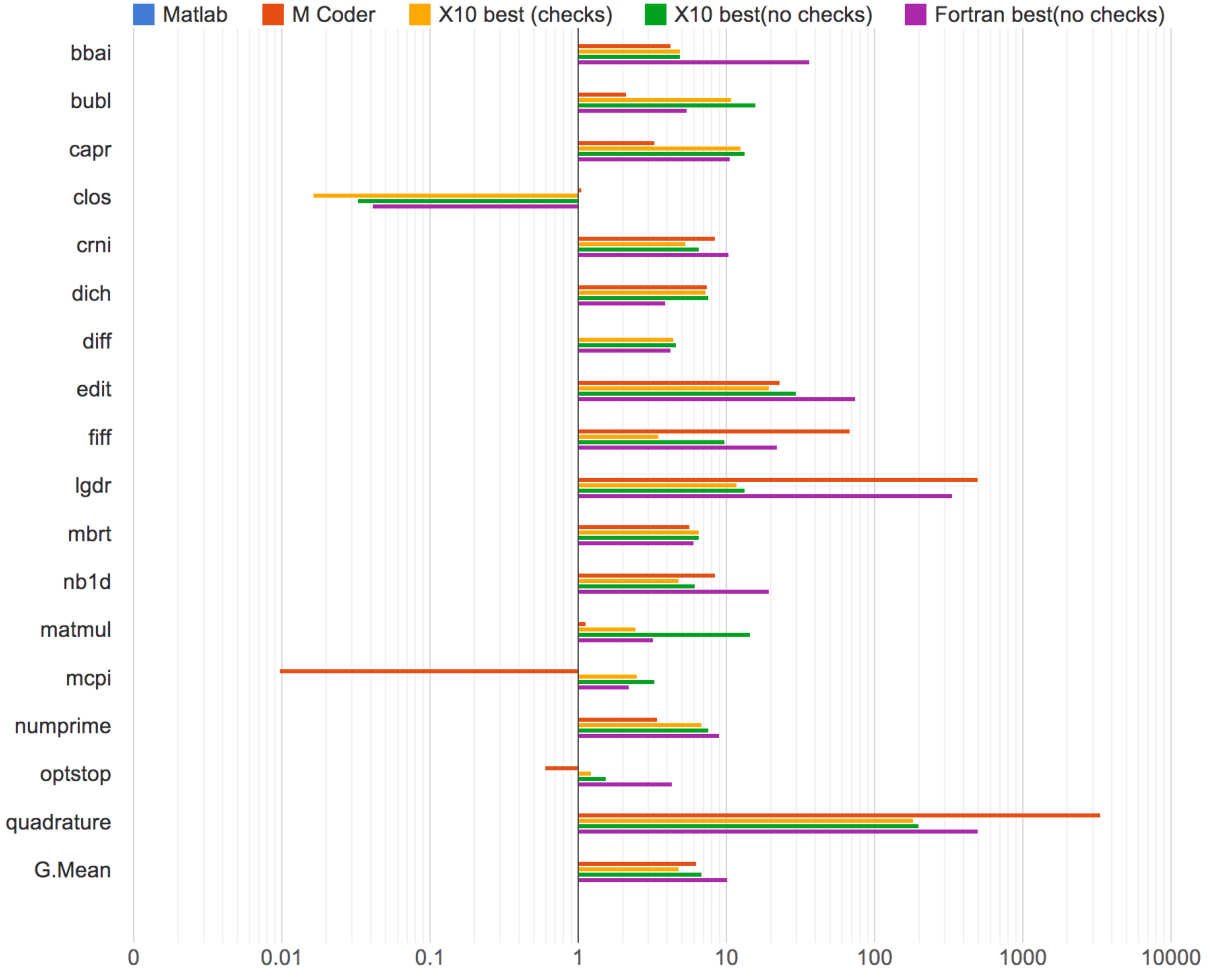
\includegraphics[width=\linewidth]{Figures/final/overall_perf.pdf}
\caption{Performance of \mixten vs other state-of-the-art static
compilers, reported as speedups relative to Mathworks' \matlab,  higher
is better.} \label{Fig:overall_perf} 
\end{center} 
\end{figure*} 

\figref{Fig:overall_perf} shows the speedups and slowdowns for the code
generated for our benchmarks by different compilers.  For \mixten we have
included the results for the \xten code compiled by the \xten C++ backend
compiled, once with \texttt{-NO\_CHECKS} enabled and once with
\texttt{-NO\_CHEKCS} disabled.  For Fortran we included the results for the
code generated without bounds checks.  C code from \matlab coder was generated
with default settings and includes bounds checks. We also calculated the
geometric mean of speedups(slowdowns) for all the benchmarks for each compiler. 

Overall, one can see that the static compilers all provide excellent
speedups, often of at least an order of magnitude faster.  Thus, for the
kinds of benchmarks in our benchmark set, it would seem that tools like
the \matlab coder, \mctwofor, and our \mixten tools are very useful.
\mixten outperforms \matlab coder in 9 out of 17 benchmarks, when
compared with the \xten version compiled with bounds checks, and 10 out
of 17 benchmarks when compared with the version with no bounds checks.
For Fortran, the generated \xten does better in 7 out of 17 benchmarks
with no bounds checks, and 6 out of 17 benchmarks with bounds checks
enabled.  Note that \matlab coder was not able to compile 1 of our
benchmarks (\emph{diff}) due to the dynamic array
growth involved in it; \mixten supports dynamic array growth.  

We achieved a mean speedup of 4.8
over \matlab, for the \xten code with bounds checks, and 6.8 for the x10 code
with no bounds checks.  On the other hand, \matlab coder gave a mean speedup of
6.3 and \mctwofor gave a mean speedup of 10.2.  However, we noticed that our
mean result was skewed due to two benchmarks for which the generated \xten
performed very poorly compared to the generated C code.  These benchmarks are
\emph{clos} and \emph{lgdr}. In the following paragraphs we explain the reason
for their poor performance.  If  we do not consider these two benchmarks, we
get a mean speedup of 6.7 for the \xten code with bounds checks compared to 5.2
for the C code. For the \xten code compiled with no bounds checks we get a mean
speedup of 9.3 compared to 11.6 for Fortran. 

\emph{clos} involves repeated calls to the builtin matrix multiplication
operation for the 2-dimensional matrices. The generated C code from \matlab
coder uses highly optimized matrix multiplication libraries compared to the
naive matrix multiplication implementation used by \mixten. Thus, \mixten gets a
speedup of 0.02 as compared to 1.05 for C. Note that the generated Fortran
code is also slowed down (speedup of 0.04) due to the same reason. As a future
work, We plan to replace our matrix multiplication implementation with calls to
an optimized library function.       

\emph{lgdr} involves repeated transpose of a row vector to a column vector.
\matlab and Fortran, both being array languages are highly optimized for
transpose operations. \mixten currently uses a naive transpose algorithm which
is not optimized. We did achieve a speedup of over 10 times compared to \matlab
but it is not as good as the speedups achieved by C (speedup of 505.0) and
Fortran (speedup of 336.7). For transpose operation also, we plan to replace
our current implementation with an optimized implementation or a call to an
optimized library function.  

Both of these examples show that in addition to generating good code,
another important task is developing optimized \xten library routines for key
array computations.

Other interesting numbers are shown by \emph{optstop},
\emph{fiff}, \emph{nb1d}, and \emph{quadrature}.  \emph{optstop} gave a speedup
of just 1.5 even without bounds checks. It involves repeated random number
generation, which our experiments showed to be slow for the \xten C++ backend
compared to Fortran and even the Java backend.  This problem is worse with C,
due to which the C code from \matlab coder gives a speedup of mere
0.6(slowdown). Fortran performs better with a speedup of 4.3.  \emph{bbai}
shows a similar pattern due to the same reason. 
\begin{comment}
 \emph{numprime} involves a for
loop over a conditional that evaluates to true only once. \matlab coder
leverages this fact for optimizing the for loop by implicitly inserting a
\texttt{break} when the conditional becomes true. C code for \emph{numprime}
provides a speedup of 792.00 compared to 6.83 for \xten and 9.00 for java.  We
tested our generated \xten code by explicitly inserting a \texttt{break}
statement and achieved a speedup of around 65 times. Note that \emph{numprime}
is also used for demonstrating \texttt{parfor} which does not allow a
\texttt{break} statement in the loop.
\end{comment}
\emph{fiff} is characterized by stencil
operations in a loop on a 2-dimensional array. These operations are also
optimized by array-based languages like Fortran and \matlab.  For \emph{nb1d},
Fortran performs better due to the use of column vectors in the benchmark, which
are represented as 2-dimensional arrays in \xten but in Fortran they are
represented as 1-dimensional and are optimized. 2-dimensional arrays are not as
fast in \xten as the 1-dimensional arrays.  \emph{quadrature} involves repeated
arithmetic calculations on a range of numbers. We achieve a speedup of about 200
times compared to \matlab, however it is slow compared to speedups of 3348 and
502 by C and Fortran respectively.  We believe that \matlab coder leverages
partial evaluation for optimizing numerical methods' implementations.

\begin{comment} VK:
 reasoning for quadrature is a speculation. I am not very sure
if this is the case. The program is really simple and there seems to be nothing
unique going on.  
\end{comment}

For most of the other benchmarks, we perform better or nearly equal to C and
Fortran code. Despite the facts that: (1) the sequential core of \xten is a
high-level object oriented language which is not specialized for array-based
operations; and (2) Generating the executable binaries via \mixten involves two
levels of source-to-source compilations (\matlab $\rightarrow$ \xten
$\rightarrow$ C++); we have achieved performance comparable to C, the state of
the art in statically compiled languages and Fortran, a statically compiled
language highly specialized for arrays.
       
\section{\xten C++ Backend vs. \xten Java Backend}

The \xten compiler provides two backends, a C++ backend that compiles the \xten
code to native binary via C++, and a Java backend that compiles the \xten code
to JVM code via Java. We were interested to see how well these backends perform
when used to compile the \mixten generated code. Even though we did not expect
Java code to perform as well as the C++ code, our aim was to make sure that we
achieved good performance, significantly better than \matlab, for the \xten
Java backend.  This would enable \matlab programmers to use our \mixten
compiler to generate code that could be integrated into Java applications. 

In this section we present the performance comparison of the \mixten
generated \xten code compiled by the \xten C++ backend with that compiled by
the \xten Java backend. Columns 3 and 4 of the Table \ref{tab:cpp_vs_java} show
speedups for our benchmarks compiled with the \xten C++ backend without bounds
checks, and with bounds checks respectively. Columns 5 and 6 show these values
for compilation with the \xten Java backend without bounds checks, and with
bounds checks respectively. We also show the geometric mean of the speedups for
all the 4 cases. 

\begin{table*}[htbp]
\begin{center} 
\begin{footnotesize}
\begin{tabular}{|r|c|c c|c c|} \hline Benchmark      & Matlab & C++ (no checks)
& C++ (checks) & Java (no checks) & Java (checks) \\ \hline bbai           & 1
& 4.9             & 4.9          & 11.3             & 10.7          \\ bubl
& 1      & 15.8            & 10.8         & 7.5              & 7.5           \\
capr           & 1      & 13.5            & 12.7         & 11.1             &
6.3           \\ clos           & 1      & 0.03            & 0.02         & 0.02
& 0.002         \\ crni           & 1      & 6.5             & 5.3          &
5.6              & 4             \\ dich           & 1      & 7.6             &
7.3          & 7                & 1.6           \\ diff           & 1      & 4.6
& 4.4          & 0.3              & 0.3           \\ edit           & 1      &
29.7            & 19.4         & 22.1             & 20            \\ fiff
& 1      & 9.8             & 3.5          & 2.1              & 1.4           \\
lgdr           & 1      & 13.5            & 11.9         & 10.6             &
10.6          \\ mbrt           & 1      & 6.5             & 6.5          & 0.3
& 0.3           \\ nb1d           & 1      & 6.2             & 4.8          &
5.5              & 4.1           \\ matmul         & 1      & 14.7            &
2.5          & 1.1              & 0.8           \\ mcpi           & 1      & 3.3
& 2.5          & 2.9              & 3             \\ numprime       & 1      &
7.6             & 6.8          & 6.5              & 6.4           \\ optstop
& 1      & 1.5             & 1.2          & 1.8              & 1.4           \\
quadrature     & 1      & 200.9           & 182.6        & 167.4            &
154.5         \\ \hline Geometric mean & 1      & 6.8             & 4.8
& 3.4              & 2.4           \\ \hline
\end{tabular}

\end{footnotesize}
\caption{\mixten performance comparison : \xten C++ backend vs. \xten
Java backend, speedups relative to Mathworks' \matlab, higher is better} 
\label{tab:cpp_vs_java} 
\end{center} 
\end{table*}

The mean speedups for the C++ backend are 6.8 and 4.8 respectively for the
version with bounds checks switched off, and the version with bounds checks
switched on, whereas for Java backend these values are 3.4 and 2.4
respectively. This is expected, given that C++ is compiled to native binary
while Java is JIT compiled. 

\emph{bbai} and \emph{optstop} are the two exceptions, where Java performs
better than C++.  For \emph{bbai}, both the Java versions gave a speedup of
over 10, whereas for C++, the speedup is under 5 for both the versions. For
\emph{optstop}, the difference is not large, with C++ speedup at 1.5 (1.2 for
the bounds checks version) compared to 1.8 (1.4 for the bounds checks
version) for the Java backend. \emph{bbai} is slower with \xten C++ backend
because it includes repeated calls to the \xten's \texttt{Random.nextDouble()}
function to generate random numbers. We found it to be significantly slower in
the C++ backend compared to the Java backend. We have reported our findings to
the \xten development team and they have validated our findings. \emph{optstop}
is slower for the same reason : It also involves repeated random number
generation. Note that for these two benchmarks, even the C code generated via
\matlab coder is slower than the C++ code, with speedups of 4.2 and 0.6
respectively for \emph{bbai} and \emph{optstop}. 

Other interesting results are for the benchmarks \emph{diff}, \emph{fiff},
\emph{mbrt} and \emph{matmul}. For these benchmarks, results from the Java
backend are significantly slower compared to the C++ backend.  \emph{diff} and
\emph{mbrt} involve operations on complex numbers. In the \xten C++ backend,
complex numbers are stored as \texttt{structs} and are kept on the stack,
whereas in the Java backend, they are stored as \emph{objects} and reside in
the heap storage.  \emph{fiff} and \emph{matmul}  are characterized by repeated
array access and read/write operations on 2-dimensional arrays.  For these
benchmarks, the Java backend performs significantly slower compared to the C++
backend with no bounds checks(2.1 vs. 9.8 for \emph{fiff} and 1.1 vs.  14.7
for \emph{matmul}), however compared to the performance by the C++ beckend with
bounds checks, it is not as slow(2.1 vs. 3.5 for \emph{fiff} and 1.1 vs.
2.5 for \emph{matmul}).  The reason is that even with bounds checks turned off
for the \xten to Java compiler, The Java compiler by default has bounds checks
on. These checks have a significant effect on performance for 2-dimensional
array operations.

\subsection{When Not to Use the \xten \texttt{-O}}
\label{sec:BOOM}

One of the most surprising results in this set of experiments was the fact that
we had to sometimes disable the \xten \texttt{-O} optimizer switch when
using the \xten Java backend..
For the benchmarks \emph{capr} and
\emph{dich}, in the case when \xten bounds checks are switched on, we found
very pathological performance, with slowdowns of over 2 orders of magntitude,
when the \xten compiler's optimization switch(\texttt{-O}) was used.

We recorded running times of 785.3 seconds for \emph{capr} compared to 3.2
seconds without the optimization, and 1558.9 seconds for \emph{dich} compared to
12.7 seconds without the optimization.  With the help of the \xten development
team we determined that switching on the optimization triggered code inlining
for the array bounds check code, which then
caused the resultant Java program to be too large to be handled by the JIT
compiler.  In fact, the Java JIT effectively gives up on this code and reverts 
to the interpreter. 

Thus, it would seem that the \xten optimizer needs to be improved in order to
apply aggressive inlining only when it does not have a negative impact on code
size,  and that different inlining strategies are needed for the C++ and Java
backends.

\section{Simple vs. Region Arrays} \label{sec:EvalArrays}

One of the key optimizations used by \mixten is to use simple arrays,
wherever possible, for higher performance.  In this section we discuss the
performance gains obtained by using simple arrays over region arrays and
the specialized region arrays.  A description of these three kinds of arrays
provided by \xten was given in \secref{subsec:ArrayDesc}.  Table
\ref{tab:simple_vs_region} shows the relative speedups and slowdowns for our
benchmarks compiled to use different kinds of \xten arrays for the C++ backend
and the Java backend.

\begin{table*}[htbp]
\begin{center} 
%\begin{footnotesize}
\scalebox{0.67}{
\begin{tabular}{|r|c|ccc|ccc|}
\hline
           &        & \multicolumn{3}{c|}{X10 C++ backend}                   &
\multicolumn{3}{c|}{X10 Java backend}                  \\ \hline
Benchmark  & Matlab & Simple arrays & Region arrays & Sp. region arrays &
Simple arrays & Region arrays & Sp. region arrays \\ \hline
bbai           & 1.0     & 4.9                    & 2.7                     & 2.7                             & 11.3                         & 6.4                      & 6.6                              \\
bubl           & 1.0     & 15.8                   & 11.4                    & 11.6                            & 7.5                          & 3.6                      & 3.7                              \\
capr           & 1.0     & 13.5                   & 11.6                    & 12.4                            & 11.1                         & 0.02                        & 10.5                             \\
clos           & 1.0     & 0.03                   & 0.01                    & 0.01                               & 0.02                         & 0.01                     & 0.01                             \\
crni           & 1.0     & 6.5                    & 3.6                     & 3.9                             & 5.6                          & 4                        & 4.1                              \\
dich           & 1.0     & 7.6                    & 6.7                     & 7.0                               & 7.0                            & 0.01                        & 0.02                                \\
diff           & 1.0     & 4.6                    & 4.2                     & 4.3                             & 0.3                          & 0.3                      & 0.3                              \\
edit           & 1.0     & 29.7                   & 4.3                     & 3.6                             & 22.1                         & 9.4                      & 9.4                              \\
fiff           & 1.0     & 9.8                    & 2.0                       & 2.8                             & 2.1                          & 1.4                      & 1.4                              \\
lgdr           & 1.0     & 13.5                   & 1.6                     & 1.5                             & 10.6                         & 5.4                      & 5.4                              \\
mbrt           & 1.0     & 6.5                    & 6.3                     & 6.5                             & 0.3                          & 5.1                      & 5.1                              \\
nb1d           & 1.0     & 6.2                    & 0.3                     & 0.3                             & 5.5                          & 1.4                      & 1.4                              \\
matmul         & 1.0     & 14.7                   & 1.3                     & 1.4                             & 1.1                          & 0.5                      & 0.5                              \\
mcpi           & 1.0     & 3.3                    & 2.8                     & 2.7                             & 2.9                          & 3.0                        & 3.0                                \\
numprime       & 1.0     & 7.6                    & 5.7                     & 5.7                             & 6.5                          & 6.3                      & 6.3                              \\
optstop        & 1.0     & 1.5                    & 0.4                     & 0.4                             & 1.8                          & 1.2                      & 1.3                              \\
quadrature     & 1.0     & 200.9                  & 200.9                   & 200.9                           & 167.4                        & 143.5                    & 154.5                            \\ \hline
Geometric mean & 1.0     & 6.8                    & 2.7                     & 2.8                             & 3.4                          & 1.3                      & 1.9  
\\ \hline                           
\end{tabular}

}
%\end{footnotesize}
\caption{\mixten performance comparison : Simple
arrays vs. Region arrays vs.  Specialized region arrays, speedup relative to 
Mathworks' \matlab, higher is better} 
\label{tab:simple_vs_region} 
\end{center}
\end{table*}

For the C++ backend we obtained a mean speedup of 6.8 for Simple arrays,
compared to 2.7 for region arrays and 2.8 for specialized region arrays. For
the Java backend, we obtained speedups of 3.4, 1.3 and 1.9 for the simple
arrays, region arrays, and the specialized region arrays respectively. These
results are as expected in \secref{Sec:CompileArrays}. For the C++ backend,
most noticeable performance differences between simple arrays and region arrays
are for \emph{edit}, \emph{fiff}, \emph{lgdr}, \emph{nb1d}, \emph{matmul} and
\emph{optstop}. All of these benchmarks are characterized by large number of
array accesses and read/write operations on 2-dimensional arrays, except
\emph{optstop} and \emph{edit}, which have multiple large 1-dimensional arrays.
The performance difference is most noticeable for \emph{nb1d}, where the region
arrays are about 20 times slower than the simple arrays. This is because
\emph{nb1d} involves simple operations on a large column vector. With simple
arrays, since the compiler knows that it is a column vector, rather than a
2-dimensional matrix, even though it is declared as a 2-dimensional array, the
performance can be optimized to match that of the underlying \texttt{Rail}.
However, this is not possible for region arrays where the size of each
dimension is not known statically. For the C++ backend, we do not observe
significant performance differences between the region arrays and the
specialized region arrays.

For the Java backend we observed a higher difference in the mean performance
for the simple arrays and the region arrays. The mean speedup for region arrays
is 1.3 whereas for simple arrays it is nearly 3 times more at 3.4. There is
also a significant difference between the performance of specialized region
arrays and region arrays. Speedup for specialized region arrays is 1.9. Like
the C++ backend, here also, most noticeable performance gain for simple arrays
is for benchmarks involving a large number of array accesses and read/writes.
\emph{capr} and \emph{dich} ask for special consideration. For \emph{capr},
even with \xten compiler's bounds checks turned off, the region array version
slows down by more than 500 times compared to the simple array version and even
the specialized region array version. This again, is due to the fact that
region arrays, with the dynamic shape checks, generated more code than the JIT
compiler could handle. For \emph{dich} the slowdown due to region arrays was
about 700 times compared to simple arrays. For \emph{dich}, even the
specialization on region arrays was not enough to reduce the code size enough
to be able to be JIT compiled. 

\section{Effect of the IntegerOkay Analysis}    
\label{sec:intok_perf}

In this section we present an overview of the performance improvements
achieved by \mixten by using the IntegerOkay analysis. Table \ref{tab:int_vs_double}
shows a comparison of speedups gained by using the IntegerOkay analysis over
those without using it. For this experiment we used results with \xten
optimizations turned on and bounds checks turned off. 
   
\begin{table*}[htbp]
\begin{center} 
\begin{footnotesize}
\begin{tabular}{|r|c|cc|cc|}
\hline
               &        & \multicolumn{2}{c|}{X10 C++ backend} &
\multicolumn{2}{c|}{X10 Java backend} \\ \hline
Benchmark      & Matlab & IntegerOkay      & All Doubles      & IntegerOkay
& All Doubles      \\ \hline
bbai       & 1.0    & 4.9             & 3.8                & 11.3                         & 8.2                 \\
bubl       & 1.0    & 15.8            & 2.2                & 7.5                          & 4.2                 \\
capr       & 1.0    & 13.5            & 1.7                & 11.1                         & 9.7                 \\
clos       & 1.0    & 0.03            & 0.02               & 0.02                         & 0.01                \\
crni       & 1.0    & 6.5             & 2.8                & 5.6                          & 5.5                 \\
dich       & 1.0    & 7.6             & 1.0                & 7.0                          & 5.8                 \\
diff       & 1.0    & 4.6             & 4.5                & 0.3                          & 0.3                 \\
edit       & 1.0    & 29.7            & 13.5               & 22.1                         & 20.0                \\
fiff       & 1.0    & 9.8             & 1.0                & 2.1                          & 1.8                 \\
lgdr       & 1.0    & 13.5            & 10.1               & 10.6                         & 11.0                \\
mbrt       & 1.0    & 6.5             & 6.1                & 0.3                          & 0.3                 \\
nb1d       & 1.0    & 6.2             & 5.2                & 5.5                          & 5.5                 \\
matmul     & 1.0    & 14.7            & 14.5               & 1.1                          & 1.2                 \\
mcpi       & 1.0    & 3.3             & 3.3                & 2.9                          & 2.9                 \\
numprime   & 1.0    & 7.6             & 7.6                & 6.5                          & 7.1                 \\
optstop    & 1.0    & 1.5             & 1.0                & 1.8                          & 1.0                 \\
quadrature & 1.0    & 200.9           & 182.6              & 167.4                        & 143.5               \\ \hline
Geometric mean         & 1.0    & 6.8             & 3.4                & 3.4                          & 2.9                 \\ \hline
\end{tabular}

\end{footnotesize}
\caption{Performance evaluation for the IntegerOkay
analysis, speedups relative to Mathworks' \matlab, higher is better} 
\label{tab:int_vs_double} 
\end{center} 
\end{table*}

For the C++ backend, we observed a mean speedup of 6.8 which is two
times the speedup gained by not using the IntegerOkay analysis, which is equal
to 3.4. We observed a significant gain in performance by using IntegerOkay
analysis for the benchmarks that involve significant number of array indexing
operations. \emph{bubl}, \emph{capr}, \emph{crni}, \emph{dich}, and \emph{fiff} 
show the most significant performance gains. The reason for this
behaviour is that, \xten requires all array indices to be of type \texttt{Long},
thus if the variables used as array indices are declared to be of type
\texttt{Double} (which is the default in \matlab), they must be typecast to
\texttt{Long} type. \texttt{Double} to \texttt{Long} is very time consuming
because every cast involves a check on the value of the \texttt{Double} type
variable to ensure that it can safely fit into \texttt{Long} type. 

For the Java backend, with the IntegerOkay analysis, we get a mean speedup of
3.4 as compared to 2.9 without it. The reason for the lower difference as
compared to that for the C++ backend is that, for Java backend, the \xten
compiler does not generate the value checks for \texttt{Double} type values,
instead it relies on the JVM to make  these checks, resulting in a better
performance.  Also note that, without the IntegerOkay analysis, the C++ backend
results are slower than the Java backend results for 9 out of 17 benchmarks.

To conclude, IntegerOkay analysis is very important for efficient performance
of code involving Arrays, specially for the \xten C++ backend.

\section{\matlab parfor vs. \mixten Parallel Code} \label{sec:parfor_results}
 
Given that we have established that we can generate competitive sequential
code, we wanted to also do a preliminary study to see if we could get
additional benefits from the high-perfomance nature of \xten.  In this section
we present the preliminary results for the compilation of \matlab
\texttt{parfor} construct to the parallel \xten code. 7 out of our 17
benchmarks could be safely modified to use the \texttt{parfor} loop.  We
compare the performance of the generated parallel \xten programs for these
benchmarks to that of \matlab code using \texttt{parfor}, and to their
sequential \xten versions. For this experiment, we used the sequential
versions of the generated \xten programs with optimizations and no bounds
checks.  For the parallel versions we used both the variants, with
optimizations and bounds checks, and with optimizations and without bounds
checks. It is important to note that the Intel(R) Core(TM) i7-3820 CPU used
for this experiment has 4 CPU cores and 8 hardware threads, thus bounding the
\xten parallelization speedup at 8. Table \ref{tab:parfor_vs_x10} shows the
results for both the \xten C++ and the
\xten Java backends.
   
\begin{table*}[htbp]
\begin{center} 
%\begin{footnotesize}
\scalebox{0.7}{
\begin{tabular}{|r|c|c|c|cc|c|cc|}
\hline
               &        &               & \multicolumn{3}{c|}{X10 C++ backend}
& \multicolumn{3}{c|}{X10 Java backend}          \\ \hline
               &        &               & Sequential &
\multicolumn{2}{c|}{Parallel}     & Sequential & \multicolumn{2}{c|}{Parallel}
\\ \hline
Benchmarks     & MATLAB & MATLAB parfor &   No checks & No checks & 
Checks &     No checks       & No checks & Checks \\ \hline
mbrt           & 1.0    & 1.7           & 6.5                            & 25.3                         & 25.3                      & 0.3                             & 1.3                           & 1.3                        \\
nb1d           & 1.0    & 0.4           & 6.2                            & 7.3                          & 7.3                       & 5.5                             & 19.0                          & 15.1                       \\
matmul         & 1.0    & 1.3           & 14.7                           &
68.7                        & 3.9                       & 1.1                             & 1.1                           & 0.8                        \\
mcpi           & 1.0    & 4.6           & 3.3                            & 15.7                         & 15.9                      & 2.9                             & 18.1                          & 18.2                       \\
numprime       & 1.0    & 5.3           & 7.6                            & 30.0                         & 30.9                      & 6.5                             & 24.8                          & 26.4                       \\
optstop        & 1.0    & 4.1           & 1.4                            & 2.0                          & 2.1                       & 1.8                             & 10.7                          & 9.7                        \\
quadrature     & 1.0    & 3.8           & 200.9                          & 11.3                         & 11.2                      & 167.4                           & 13.0                          & 13.0                       \\ \hline
Geometric mean & 1.0    & 2.3           & 8.9                            &
14.5                         & 9.8                       & 3.7                             & 7.8                           & 7.1                        \\ \hline
\end{tabular}
 
%\end{footnotesize}
}
\caption{Performance evaluation for \mixten generated
parallel \xten code for the \matlab \texttt{parfor} construct, speedups
relative to Mathworks' \matlab,  higher is better} 
\label{tab:parfor_vs_x10} 
\end{center} 
\end{table*}

For the \xten C++ backend we achieved a mean speedup of 14.5 for the generated
parallel \xten code without bounds checks, which is around 7 times of the
speedup for the \matlab code with \texttt{parfor}, at a speedup of 2.3.
Compared to \xten sequential code which has a mean speedup of 8.9, it is more
than 1.5 times as fast.  Even with the parallel \xten code with bounds checks
we achieved a speedup of 9.8 which is over 4 times better than the \matlab
\texttt{parfor} code. The \emph{optstop} benchmark is an interesting
exception. It is actually slower (at a speedup of 2.1) than the \matlab
\texttt{parfor} version (at a speedup of 4.1). The sequential version of
\emph{optstop} is just slightly faster than the sequential \matlab version,
with a speedup of just 1.5 (due to the reasons explained earlier in
\secref{sec:XXX}) and the total time for the parallel execution of each
iteration, and managing the parallelization of these activities is just
slightly faster than the sequential version. We see a similar trend for the
\emph{matmul} benchmark for the \xten Java backend. It shows a speedup of just
0.8 (version with bounds checks) as compared to 1.3 for the \matlab
\texttt{parfor} version. For the parallel version of \emph{matmul}, the
speedup for the C++ backend with checks turned on is just 3.9 compared to 14.7
for the sequential version with no checks, however it is 1.6 times faster than
the sequential version with checks, which has a speedup of just 2.5 (shown in
figure \ref{Fig:overall_perf}). The \emph{quadrature} benchmark shows very
interesting numbers, with a slowdown of about 20 times and 13 times for the
parallel \xten code compared to the sequential \xten code, for the C++ backend
and the Java backend respectively. The \emph{quadrature} benchmark consists of
a loop with a large number of iterations (4600000 for our experiment), where
each iteration performs an insignificant amount of computations with just 21
simple arithmetic operations on scalar values. A sequential speedup of over
200 times compared to the sequential \matlab code indicates the insignificance
of each iteration in terms of computation time. In the parallel \xten code,
each iteration is executed as a separate activity, and the time taken to
manage the large number of activities overshadows the sequential speedup.
Also, each activity has an \texttt{atomic} statement, which is a blocking
construct (when one activity is executing the atomic statement, all other
activities are blocked) and adds further overhead to the activity management
system. Performance numbers for \emph{quadrature} assert the fact that not all
parallel \matlab programs are good candidates to be compiled to parallel \xten
in a straight-forward fashion, specially the ones with large number of
parallel loop iterations where each iteration itself does insignificant amount
of work. As a future work, we plan to handle such programs with more
sophisticated parallelization techniques. For example, one way to make a
benchmark like \emph{quadrature} more efficient would be to break the loop into
two nested loops and executing the outer loop in a parallel fashion and the
inner loop sequentially to ensure that each concurrent loop does substantial
amount of work, however the challenge here is to determine the right number of
iterations for the inner sequential loop to make it significant enough to take
advantage of the parallelization.           

Overall for the Java backend, we obtained a mean speedup of 7.8 for the \xten
code with no bounds checks and 7.1 for the code with bounds checks. Compared
to the \matlab parfor version we obtained about 3.5 times better performance.
The parallel \xten code is over 2 times faster than the sequential \xten code
(speedup of 3.7). For both, the C++ backend, and the Java backend, the mean
speedup for the sequential \xten code is also substantially faster than the
\matlab parallel code.  

To conclude, the parallel \xten code provides much higher performance
gains compared to the \matlab \texttt{parfor} code  and even the \xten
sequential code, which by itself is most of the times faster than the
\matlab parallel code.


\section{Summary}

We showed that the \mixten compiler with its efficient handling of array
operations and optimizations like IntegerOkay can generate \xten code
that provides performance comparable to the native code generated by the
state of the art languages like C, which is fairly low-level, and
Fortran, which itself is an array-based language.  As a future work, we
plan to use more efficient implementations of the builtin functions, and
believe that it would further improve the performance of the code
generated by \mixten.

With \mixten, we also took first steps to compile \matlab to parallel
\xten code to take full advantage of the high performance features of
\xten. Our preliminary results are very inspiring and we plan to
continue in this direction further, in the future.

In addition to demonstrating that our approach leads to good code, these
experiments have also been quite valuable for the \xten development team.
Our generated code has stressed the \xten system more than the
hand-written \xten benchmarks and has exposed places where further
improvements can be made.


\chapter{Related Work} \label{chap:Related}
The work in this thesis presents a research compiler for \matlab. 
We provide a source-to-source static
compiler that targets the high-level, object oriented language, \xten.  Our approach is
open and extensible and generates sequential \xten code that is competitive in
performance to code in state-of-the-art languages like C and Fortran, generated
by other \matlab compilers. We also generated high performance code for
\matlab's \texttt{parfor} loops, that showed great performance improvements.

\section{Alternatives to \matlab}
Although our focus is on handling \matlab itself, there are notable open source
alternatives of \matlab like Scilab\cite{Scilab}, Julia\cite{julia},
NumPy\cite{numpy}, FreeMat\cite{freemat} and Octave\cite{Octave}.
Octave is an open source implementation of the \matlab language and supports
most of the \matlab programs, however until the recently released version 3.8.1,
Octave was solely an interpreted language and our experiments showed it to be
orders of magnitude slower than \matlab. We would like to evaluate its
performance for the latest version that comes with a JIT compiler. Scilab and
FreeMat are similar in syntax to \matlab but have significant differences that
prevent a significant portion of \matlab programs to be able to run on these systems.
NumPy is a python package for scientific computing, and Julia is a technical
computing language. Julia also provides a fairly advanced distributed parallel
execution environment. However, these alternative systems concentrate on
providing open library support and have not tackled the problems of static
compilation.  We are investigating if there is any way of
sharing some of their library support with \mixten. A Comparative evaluation of
Matlab, Octave, FreeMat, Scilab, R, and IDL on a cluster computing system is 
presented in a technical report by Coman at al.~\cite{coman}  
The MEGHA
project\cite{megha} provides an interesting approach to map \matlab array
operations to CPUs and GPUs, but supports only a very small subset of \matlab.  

%As discussed in \secref{Sec:Background}, this work builds upon the
%previous work from the \mclab group, including the front-end, the \mcsaf
%analysis framework~\cite{JesseThesis,McSAFecoop12} analysis framework,
%and the \matlab Tamer~\cite{TamerPaper}.

\section{Other \matlab Compilers}
There have been  previous research projects on static compilation of
\matlab which focused particularly on the array-based subset of \matlab
and developed advanced static analyses for determining shapes and sizes
of arrays.  For example, FALCON \cite{falcon} is a \matlab to {\sc
Fortran90} translator with sophisticated type inference algorithms.
The McLab group has previously implemented a prototype Fortran 95
generator~\cite{McForThesis}, and has more recently developed the next generation
Fortran generator, \mctwofor~\cite{mc2for} in parallel with the \mixten project.   Some of the
solutions are shared between the projects, especially the parts which
extend the Tamer. \matlab Coder is a commercial compiler by MathWorks\cite{MATLABCoder},
which produces C code for a subset of \matlab. We also compared \mixten's
performance to \matlab coder. Below are more details about these and few other
notable \matlab compiler research projects:
\begin{itemize}
\item Falcon is a \matlab-to-Fortran 90 compiler that applies type inference
algorithms developed for the array programming language
APL~\cite{magica,805380,801218} and set
language SETL~\cite{361235}. It uses a static single-assignment(SSA) based
intermediate representation, and inlines all functions and scripts into one
large function. The Falcon project also curated a set of \matlab benchmarks to
measure the performance of their compiler. Several of our benchmarks are
originally from Falcon's benchmark suite.
\item \mcfor is a prototype \matlab-to-Fortran 95 generator developed by the
\mclab research group and paved way for further research (of which \mixten is a
part) into developing efficient static \matlab compilers for \matlab. \mctwofor
is the second generation \matlab-to-Fortran 95 compiler built on top of the
Tamer and \mcsaf static analysis tools. \mixten and \mctwofor share some of the
solutions that extend the Tamer tool. We have also used \mctwofor for our
performance evaluation. A good performance by both \mixten and \mctwofor further
validates the strength of our compilation techniques.
\item MAJIC (\matlab Just-In-time Compiler)~\cite{MaJIC} is a continuation of the
Falcon project. It aims to exploit optimization opportunities in the following
three areas\footnote{\url{http://polaris.cs.uiuc.edu/majic/techniques.html}}:
(1) source-level optimizations for matrix-based operations; (2) just-in-time
compilation to defer compilation as much as possible and thus minimize the
effects of challenges raised by \matlab's "wild" nature as we discussed in
\chapref{chap:CodegenSeq}; and (3) specialized optimizations for operations on
sparse matrices.
\item \textsc{Menhir}~\cite{745866} is a retargetable \matlab compiler that can
generate C or Fortran code based on a target system description(MTSD). MTSD
describes target system's properties and implementation details and thus allows
efficient code generation that exploits optimized sequential and parallel
libraries. 
\item MATCH~\cite{MAT2C} is a library based compilation environment for distributed
heterogeneous adaptive computing systems consisting of field-programmable gate
arrays and digital signal processors. It parallelizes \matlab code based on user
directives and generates C code that can call different runtime libraries. 
\item Otter~\cite{Quinn} is a \matlab to C compiler that targets parallel computers
supporting parallel numerical libraries like ScaLAPACK~\cite{898821}. It would be interesting,
as a future work, to compare performance of the Otter compiler to that of
\mixten when it supports the parallel compilation of \matlab more effectively.
\end{itemize}      

A major difference between \mixten and these compilers is that \mixten targets
an object oriented language with high-level array abstractions, and which is 
itself source-to-source compiled, whereas all the above mentioned projects either target
 JIT compilation or static compilation to either Fortran, which is itself an array
based language and in fact was the precursor of \matlab, or C, which is a fairly
low-level language with advanced native compilers. 
Even though some of the techniques used by
these compilers were helpful in generating \xten code for simple \matlab constructs,
the novelty of \mixten lies in the fact that it identified major challenges
involved in efficiently compiling \matlab arrays and array based operations to 
\xten and achieved a performance comparable to that of compilers targeting 
C and Fortran.      

\section{Compilers Targeting \xten} In terms of source-to-source compilers for
\xten, we are aware of two other projects.  StreamX10 is a stream programming
framework based on \xten~\cite{Wei-2012}.  StreamX10  consists of a stream
programming language COStream and a compiler which translates programs in
COStream to parallel \xten code.  Tetsu discusses the design of a Ruby-based DSL
for parallel programming that is compiled to \xten~\cite{Tetsu-2011}. Both these
projects focus on compiling a parallel programming language to \xten, a more
efficient and generic parallel programming language. In the future, we would like to study
these projects in more depth and hope to get useful insights into efficiently
using \xten as a target language for parallelism in \matlab.
 


\chapter{Conclusions and Future Work} \label{chap:Conclusions}
\section{Conclusions}
This thesis is about providing a bridge between two communities,  the
scientists/engineers/students who like to program in \matlab on one
side;  and the programming language and compiler community who have
designed elegant languages and powerful compiler techniques on the other
side.   

The \xten language has been designed to provide high-level  array and
concurrency abstractions,  and  our main goal was to develop a tool that
would allow programmers to automatically convert their \matlab code to
efficient \xten code.    In this way programmers can port their existing
\matlab code to \xten,  or continue to develop in \matlab and use our
\mixten compiler as a backend to generate \xten code.    Since \xten is
publicly available under the Eclipse Public License
(\url{x10-lang.org/home/x10-license.html}),  users could have efficient
high-performance code that they could freely distribute.    Further,
\xten itself can compile the code to either Java or C++,  so our tool
could be used in a tool chain to convert \matlab to those languages as
well.

Our tool is part of the McLab project, which is entirely open
source.   Thus, we are providing  an infrastructure for other compiler
researchers to build upon this work,  or to use some of our approaches
to handle other popular languages such as R.

In this thesis we demonstrated the end-to-end organization of the \mixten
tool, and we identified that the correct handling of arrays, the
minimization of casting by safely mapping \matlab double variables to
\xten integer variables via \emph{IntegerOkay} analysis,  and handling concurrency
features were the key challenges.   We developed a custom version of \xten's
rail-backed simple arrays,  and identified where and how this
could be used for generating efficient \xten code.  For cases where
precise static array shape and type information is not available, we
showed how we can use the very flexible region-based arrays in \xten,
and our experiments demonstrated that it is very important to use the
simple rail-backed arrays, for both the Java and C++ backends for \xten.

Our experiments show that our generated \xten code is competitive with
other state-of-the art code generators which target more traditional
languages like C and Fortran.   The C++ \xten backend produces faster
code than the Java backend,  but good performance is achieved in both
cases.  

One of the main motivations of choosing \xten as the target language is
that it supports high-performance computing,  which is often desirable
for the computation-intensive applications developed by the engineers
and scientists.   To demonstrate how to take advantage of \xten's
concurrency, we presented 
an effective translation of the \matlab \texttt{parfor} construct to
semantically equivalent \xten.    

Our experiments showed significant performance gains for our generated
parallel \xten code, as compared to \matlab's parallel toolbox. This
confirms that compiling \matlab to a modern high-performance language
can lead to significant performance improvements. 

In the process of developing \mixten, we also stressed the \xten compiler with
machine generated code and found it to be mostly robust and efficient. We found
that the \xten Java backend's optimizations may in some cases generate Java code
that is too large to be JIT compiled. We also found the random number generation
for the C++ backend to be slower than that for the Java backend. We reported our
feedback to the \xten development team and hope that our findings would help to
make \xten even better. Overall, we found that with the right techniques, \xten
can be used as an effective and efficient target language for scientific and
array-based languages, for both, the sequential core and the parallel part.   

\section{Future Work}
Based on our positive experiences to date,  we plan to continue
improving the \mixten tool.  There are three major areas where we plan to take
ahead the development of \mixten, with the aim of making it more complete and
more efficient:
\begin{description}

\item[Exploiting parallelism] To help us better understand and efficiently
exploit the inherent concurrency in the \matlab programs, first of all we would 
like to thoroughly evaluate and fine tune
the concurrency constructs we introduced in \matlab via structured comments, and
parallelism of the vectorized operations. Further, we would like to experiment
to find the best way to tune the generated code for different
sorts of parallel architectures. We are also planning to further our research
into the direction of automatically parallelizing \matlab codes through
static analysis mixed with run-time checks.   

\item[Efficient builtin implementation] One of the greatest strengths of
\matlab is its \ large and efficient set of
builtin libraries. This thesis concentrates more on effective and efficient
compilation of \matlab constructs than finding the most efficient
\xten implementations for the builtin operations. However, our experiments showed that there
are some key library routines such as matrix multiply and transpose for
which we need to have better \xten code for. Thus, there is scope for more
work on \xten libraries, which could also be useful for other
source-to-source compilers targeting \xten.

\item[Readability] The code that we generate is already quite
clean, but has a quite low-level structure, which might not be easily readable for
non-experienced \xten programmers. We would like to apply further transformations on it to
aggregate some low-level expressions, and to make the generated code
look as ``natural" as possible. This would help \mixten users, who are familiar
with \xten, to easily
fine-tune the generated \xten code to better suite their execution environments.
It would also help in easy maintenance of the generated \xten code, and better
integration with hand-written \xten code.   

\end{description}

Our tool is open source, and we hope that the other research teams will use
our infrastructure, as well as learn from our experiences of generating
effective and efficient \xten code.


% -- Bibliography -------------------------------------------------------------

%\addtocontents{toc}{\protect\addvspace{10pt}}

%\bibliographystyle{plain}

\bibliographystyle{web-alpha} %- originally in jesse thesis
%\bibliography{strings, thesis}
\bibliography{progtools,matlab,jun,refs,refs_short}


\appendix % -- Appendices -----------------------------------------------------

\addtocontents{toc}{\protect\addvspace{10pt}}
\addtocontents{toc}{\protect\contentsline{part}{Appendices}{}{}}
% -> extra {} for hyperref
%\label{TODO} % stub label for undetermined ref

\chapter{XML structure for builtin framework} \label{chap:Builtinxml}
The below listing gives the XML structure for the builtin operation
\texttt{plus}. It contains two upper level nodes for each real and complex
numbers. Each of these have specialization nodes for the simple arrays of
different dimensions, and
the region arrays. Each of the specializations has 5 types of implementations.

\begin{lstlisting}[language=X10]
<plus>
  <real>
    <simple_array>
      <array_1>
         <type1>
          {
            val x: Double;
            x = a+b;
            return x;
          }
        </type1>
        <type2>
          {a.rank == b.rank}{
            val x = new Array[Double](a.region);
              for (p in a.indices()){
                x(p) = a(p)+ b(p);
              }
              return x;
          } 
        </type2>
        <type3>
          {
            val x = new Array[Double](b.region);
            for (p in b.region){
              x(p) = a+ b(p);
            }
            return x;
          }
        </type3>
        <type4>
          {
            val x = new Array[Double](a.region);
            for (p in a.region){
              x(p) = a(p)+ b;
            }
            return x;
          }
        </type4>
        <type5>
        </type5>
      </array_1>
      <array_2>
        <type1>
          {
            val x: Double;
            x = a+b;
            return x;
          }
        </type1>
        <type2>
          {a.rank == b.rank}{
            val x = new Array[Double](a.region);
              for (p in a.indices()){
                x(p) = a(p)+ b(p);
              }
              return x;
          } 
        </type2>
        <type3>
          {
            val x = new Array[Double](b.region);
            for (p in b.region){
              x(p) = a+ b(p);
            }
            return x;
          }
        </type3>
        <type4>
          {
            val x = new Array[Double](a.region);
            for (p in a.region){
              x(p) = a(p)+ b;
            }
            return x;
          }
        </type4>
        <type5>
        </type5>
      </array_2>
      <array_3>
        <type1>
          {
            val x: Double;
            x = a+b;
            return x;
          }
        </type1>
        <type2>
          {a.rank == b.rank}{
            val x = new Array[Double](a.region);
              for (p in a.indices()){
                x(p) = a(p)+ b(p);
              }
              return x;
          } 
        </type2>
        <type3>
          {
            val x = new Array[Double](b.region);
            for (p in b.region){
              x(p) = a+ b(p);
            }
            return x;
          }
        </type3>
        <type4>
          {
            val x = new Array[Double](a.region);
            for (p in a.region){
              x(p) = a(p)+ b;
            }
            return x;
          }
        </type4>
        <type5>
        </type5>
      </array_3>
    </simple_array>
    <region_array>
        <type1>
          {
            val x: Double;
            x = a+b;
            return x;
          }
        </type1>
        <type2>
          {a.rank == b.rank}{
            val x = new Array[Double](a.region);
              for (p in a.region){
            x(p) = a(p)+ b(p);
            }
            return x;
          } 
      </type2>
      <type3>
        {
          val x = new Array[Double](b.region);
          for (p in b.region){
            x(p) = a+ b(p);
          }
          return x;
        }
      </type3>
      <type4>
        {
          val x = new Array[Double](a.region);
          for (p in a.region){
            x(p) = a(p)+ b;
          }
          return x;
        }
      </type4>
        <type5>
        </type5>
    </region_array>
  </real>
  <complex>
    <simple_array>
      <array_1>
         <type1>
          {
            val x: Double;
            x = a+b;
            return x;
          }
        </type1>
        <type2>
          {a.rank == b.rank}{
            val x = new Array[Double](a.region);
              for (p in a.indices()){
                x(p) = a(p)+ b(p);
              }
              return x;
          } 
        </type2>
        <type3>
          {
            val x = new Array[Double](b.region);
            for (p in b.region){
              x(p) = a+ b(p);
            }
            return x;
          }
        </type3>
        <type4>
          {
            val x = new Array[Double](a.region);
            for (p in a.region){
              x(p) = a(p)+ b;
            }
            return x;
          }
        </type4>
        <type5>
        </type5>
      </array_1>
      <array_2>
        <type1>
          {
            val x: Double;
            x = a+b;
            return x;
          }
        </type1>
        <type2>
          {a.rank == b.rank}{
            val x = new Array[Double](a.region);
              for (p in a.indices()){
                x(p) = a(p)+ b(p);
              }
              return x;
          } 
        </type2>
        <type3>
          {
            val x = new Array[Double](b.region);
            for (p in b.region){
              x(p) = a+ b(p);
            }
            return x;
          }
        </type3>
        <type4>
          {
            val x = new Array[Double](a.region);
            for (p in a.region){
              x(p) = a(p)+ b;
            }
            return x;
          }
        </type4>
        <type5>
        </type5>
      </array_2>
      <array_3>
        <type1>
          {
            val x: Double;
            x = a+b;
            return x;
          }
        </type1>
        <type2>
          {a.rank == b.rank}{
            val x = new Array[Double](a.region);
              for (p in a.indices()){
                x(p) = a(p)+ b(p);
              }
              return x;
          } 
        </type2>
        <type3>
          {
            val x = new Array[Double](b.region);
            for (p in b.region){
              x(p) = a+ b(p);
            }
            return x;
          }
        </type3>
        <type4>
          {
            val x = new Array[Double](a.region);
            for (p in a.region){
              x(p) = a(p)+ b;
            }
            return x;
          }
        </type4>
        <type5>
        </type5>
      </array_3>
    </simple_array>
    <region_array>
        <type1>
          {
            val x: Double;
            x = a+b;
            return x;
          }
        </type1>
        <type2>
          {a.rank == b.rank}{
            val x = new Array[Double](a.region);
              for (p in a.region){
            x(p) = a(p)+ b(p);
            }
            return x;
          } 
      </type2>
      <type3>
        {
          val x = new Array[Double](b.region);
          for (p in b.region){
            x(p) = a+ b(p);
          }
          return x;
        }
      </type3>
      <type4>
        {
          val x = new Array[Double](a.region);
          for (p in a.region){
            x(p) = a(p)+ b;
          }
          return x;
        }
      </type4>
        <type5>
        </type5>
    </region_array>
  </complex>
</plus>
\end{lstlisting}



%\chapter{Class Propagation Tables for \matlab Builtin Functions} \label{chap:allTables}
% \renewcommand{\tabcolsep}{3pt}
In this appendix we show the generated mclass propagation tables
for builtins. We categorized the functions into sections
grouping similar functions together. This categorization helped
us organize the builtin functions into a tree structure.

Rows in the tables 
correspond to the mclass of the first argument, columns correspond to
the mclass of the second argument, and the table entries give the mclass
of the result. The labels {\tt i8} through {\tt i64} represent the
mclasses {\tt int8} through {\tt int64}, {\tt f32} is {\tt single},
{\tt f64} is {\tt double}, {\tt c} is {\tt char}, and {\tt b} is {\tt
logical}. {\tt h} refers to function handles. Values labelled {\tt \{\}} refer to the
empty cell array - we use this argument to check whether functions
support cell arrays at all. Some functions allow arbitrary cell arrays,
others only operate on cell arrays of strings (e.g. the string functions).

Entries of the form ``-" indicate that this combination is
not allowed and will result in a runtime error. {\tt N/A} signifies
that the results were inconsistent across different trials, meaning
that there was no exact result found.


\newpage
\section{Binary Arithmetic Operations}

\textbf{plus, minus, mtimes, times, kron, @(x,y)cross([x,x,x],[y,y,y]):}
\begin{scriptsize}\begin{tt}\begin{center}\vspace{-.3cm}\begin{tabular}{|m{.65cm}||m{.65cm}|m{.65cm}|m{.65cm}|m{.65cm}|m{.65cm}|m{.65cm}|m{.65cm}|m{.65cm}|m{.65cm}|m{.65cm}|m{.65cm}|m{.65cm}|m{.65cm}|m{.65cm}|}\hline 
&i8&u8&i16&u16&i32&u32&i64&u64&f32&f64&c&b&h&\{\}\\ \hline \hline
i8&i8&-&-&-&-&-&-&-&-&i8&i8&-&-&-\\ \hline
u8&-&u8&-&-&-&-&-&-&-&u8&u8&-&-&-\\ \hline
i16&-&-&i16&-&-&-&-&-&-&i16&i16&-&-&-\\ \hline
u16&-&-&-&u16&-&-&-&-&-&u16&u16&-&-&-\\ \hline
i32&-&-&-&-&i32&-&-&-&-&i32&i32&-&-&-\\ \hline
u32&-&-&-&-&-&u32&-&-&-&u32&u32&-&-&-\\ \hline
i64&-&-&-&-&-&-&i64&-&-&i64&i64&-&-&-\\ \hline
u64&-&-&-&-&-&-&-&u64&-&u64&u64&-&-&-\\ \hline
f32&-&-&-&-&-&-&-&-&f32&f32&f32&f32&-&-\\ \hline
f64&i8&u8&i16&u16&i32&u32&i64&u64&f32&f64&f64&f64&-&-\\ \hline
c&i8&u8&i16&u16&i32&u32&i64&u64&f32&f64&f64&f64&-&-\\ \hline
b&-&-&-&-&-&-&-&-&f32&f64&f64&f64&-&-\\ \hline
h&-&-&-&-&-&-&-&-&-&-&-&-&-&-\\ \hline
\{\}&-&-&-&-&-&-&-&-&-&-&-&-&-&-\\ \hline
\end{tabular}\end{center}\end{tt}\end{scriptsize} 


\textbf{mldivide, mrdivide, ldivide, rdivide, mod, rem, mod:}
\begin{scriptsize}\begin{tt}\begin{center}\vspace{-.3cm}\begin{tabular}{|m{.65cm}||m{.65cm}|m{.65cm}|m{.65cm}|m{.65cm}|m{.65cm}|m{.65cm}|m{.65cm}|m{.65cm}|m{.65cm}|m{.65cm}|m{.65cm}|m{.65cm}|m{.65cm}|m{.65cm}|}\hline 
&i8&u8&i16&u16&i32&u32&i64&u64&f32&f64&c&b&h&\{\}\\ \hline \hline
i8&i8&-&-&-&-&-&-&-&-&i8&i8&-&-&-\\ \hline
u8&-&u8&-&-&-&-&-&-&-&u8&u8&-&-&-\\ \hline
i16&-&-&i16&-&-&-&-&-&-&i16&i16&-&-&-\\ \hline
u16&-&-&-&u16&-&-&-&-&-&u16&u16&-&-&-\\ \hline
i32&-&-&-&-&i32&-&-&-&-&i32&i32&-&-&-\\ \hline
u32&-&-&-&-&-&u32&-&-&-&u32&u32&-&-&-\\ \hline
i64&-&-&-&-&-&-&i64&-&-&i64&i64&-&-&-\\ \hline
u64&-&-&-&-&-&-&-&u64&-&u64&u64&-&-&-\\ \hline
f32&-&-&-&-&-&-&-&-&f32&f32&f32&f32&-&-\\ \hline
f64&i8&u8&i16&u16&i32&u32&i64&u64&f32&f64&f64&f64&-&-\\ \hline
c&i8&u8&i16&u16&i32&u32&i64&u64&f32&f64&f64&f64&-&-\\ \hline
b&-&-&-&-&-&-&-&-&f32&f64&f64&-&-&-\\ \hline
h&-&-&-&-&-&-&-&-&-&-&-&-&-&-\\ \hline
\{\}&-&-&-&-&-&-&-&-&-&-&-&-&-&-\\ \hline
\end{tabular}\end{center}\end{tt}\end{scriptsize} 

\newpage
\textbf{mpower, power:}
\begin{scriptsize}\begin{tt}\begin{center}\vspace{-.3cm}\begin{tabular}{|m{.65cm}||m{.65cm}|m{.65cm}|m{.65cm}|m{.65cm}|m{.65cm}|m{.65cm}|m{.65cm}|m{.65cm}|m{.65cm}|m{.65cm}|m{.65cm}|m{.65cm}|m{.65cm}|m{.65cm}|}\hline 
&i8&u8&i16&u16&i32&u32&i64&u64&f32&f64&c&b&h&\{\}\\ \hline \hline
i8&i8&-&-&-&-&-&-&-&-&-&i8&-&-&-\\ \hline
u8&-&u8&-&-&-&-&-&-&-&-&u8&-&-&-\\ \hline
i16&-&-&i16&-&-&-&-&-&-&-&i16&-&-&-\\ \hline
u16&-&-&-&u16&-&-&-&-&-&-&u16&-&-&-\\ \hline
i32&-&-&-&-&i32&-&-&-&-&-&i32&-&-&-\\ \hline
u32&-&-&-&-&-&u32&-&-&-&-&u32&-&-&-\\ \hline
i64&-&-&-&-&-&-&i64&-&-&-&i64&-&-&-\\ \hline
u64&-&-&-&-&-&-&-&u64&-&-&u64&-&-&-\\ \hline
f32&-&-&-&-&-&-&-&-&f32&f32&f32&f32&-&-\\ \hline
f64&i8&u8&i16&u16&i32&u32&i64&u64&f32&f64&f64&f64&-&-\\ \hline
c&i8&u8&i16&u16&i32&u32&i64&u64&f32&f64&f64&f64&-&-\\ \hline
b&-&-&-&-&-&-&-&-&f32&f64&f64&-&-&-\\ \hline
h&-&-&-&-&-&-&-&-&-&-&-&-&-&-\\ \hline
\{\}&-&-&-&-&-&-&-&-&-&-&-&-&-&-\\ \hline
\end{tabular}\end{center}\end{tt}\end{scriptsize} 




\section{Unary Arithmetic/Numeric Functions}

\textbf{uplus, uminus, real, imag, abs, fix:}
\begin{scriptsize}\begin{tt}\begin{center}\vspace{-.3cm}\begin{tabular}{|m{.65cm}||m{.65cm}|m{.65cm}|m{.65cm}|m{.65cm}|m{.65cm}|m{.65cm}|m{.65cm}|m{.65cm}|m{.65cm}|m{.65cm}|m{.65cm}|m{.65cm}|m{.65cm}|m{.65cm}|}\hline 
&i8&u8&i16&u16&i32&u32&i64&u64&f32&f64&c&b&h&\{\}\\ \hline \hline
&i8&u8&i16&u16&i32&u32&i64&u64&f32&f64&f64&f64&-&-\\ \hline
\end{tabular}\end{center}\end{tt}\end{scriptsize} 

\textbf{conj, round, floor, ceil, sign:}
\begin{scriptsize}\begin{tt}\begin{center}\vspace{-.3cm}\begin{tabular}{|m{.65cm}||m{.65cm}|m{.65cm}|m{.65cm}|m{.65cm}|m{.65cm}|m{.65cm}|m{.65cm}|m{.65cm}|m{.65cm}|m{.65cm}|m{.65cm}|m{.65cm}|m{.65cm}|m{.65cm}|}\hline 
&i8&u8&i16&u16&i32&u32&i64&u64&f32&f64&c&b&h&\{\}\\ \hline \hline
&i8&u8&i16&u16&i32&u32&i64&u64&f32&f64&f64&-&-&-\\ \hline
\end{tabular}\end{center}\end{tt}\end{scriptsize} 


\section{Operations Resulting in Logicals}

\textbf{not, any, all, isinf:}
\begin{scriptsize}\begin{tt}\begin{center}\vspace{-.3cm}\begin{tabular}{|m{.65cm}||m{.65cm}|m{.65cm}|m{.65cm}|m{.65cm}|m{.65cm}|m{.65cm}|m{.65cm}|m{.65cm}|m{.65cm}|m{.65cm}|m{.65cm}|m{.65cm}|m{.65cm}|m{.65cm}|}\hline 
&i8&u8&i16&u16&i32&u32&i64&u64&f32&f64&c&b&h&\{\}\\ \hline \hline
&b&b&b&b&b&b&b&b&b&b&b&b&-&-\\ \hline
\end{tabular}\end{center}\end{tt}\end{scriptsize} 

\textbf{isempty, isobject, isfloat, isinteger, islogical, isstruct, iscell:}
\begin{scriptsize}\begin{tt}\begin{center}\vspace{-.3cm}\begin{tabular}{|m{.65cm}||m{.65cm}|m{.65cm}|m{.65cm}|m{.65cm}|m{.65cm}|m{.65cm}|m{.65cm}|m{.65cm}|m{.65cm}|m{.65cm}|m{.65cm}|m{.65cm}|m{.65cm}|m{.65cm}|}\hline 
&i8&u8&i16&u16&i32&u32&i64&u64&f32&f64&c&b&h&\{\}\\ \hline \hline
&b&b&b&b&b&b&b&b&b&b&b&b&b&b\\ \hline
\end{tabular}\end{center}\end{tt}\end{scriptsize} 

\newpage
\textbf{eq, ne, lt, gt, le, ge, and, or, xor:}
\begin{scriptsize}\begin{tt}\begin{center}\vspace{-.3cm}\begin{tabular}{|m{.65cm}||m{.65cm}|m{.65cm}|m{.65cm}|m{.65cm}|m{.65cm}|m{.65cm}|m{.65cm}|m{.65cm}|m{.65cm}|m{.65cm}|m{.65cm}|m{.65cm}|m{.65cm}|m{.65cm}|}\hline 
&i8&u8&i16&u16&i32&u32&i64&u64&f32&f64&c&b&h&\{\}\\ \hline \hline
i8&b&b&b&b&b&b&b&b&b&b&b&b&-&-\\ \hline
u8&b&b&b&b&b&b&b&b&b&b&b&b&-&-\\ \hline
i16&b&b&b&b&b&b&b&b&b&b&b&b&-&-\\ \hline
u16&b&b&b&b&b&b&b&b&b&b&b&b&-&-\\ \hline
i32&b&b&b&b&b&b&b&b&b&b&b&b&-&-\\ \hline
u32&b&b&b&b&b&b&b&b&b&b&b&b&-&-\\ \hline
i64&b&b&b&b&b&b&b&b&b&b&b&b&-&-\\ \hline
u64&b&b&b&b&b&b&b&b&b&b&b&b&-&-\\ \hline
f32&b&b&b&b&b&b&b&b&b&b&b&b&-&-\\ \hline
f64&b&b&b&b&b&b&b&b&b&b&b&b&-&-\\ \hline
c&b&b&b&b&b&b&b&b&b&b&b&b&-&-\\ \hline
b&b&b&b&b&b&b&b&b&b&b&b&b&-&-\\ \hline
h&-&-&-&-&-&-&-&-&-&-&-&-&-&-\\ \hline
\{\}&-&-&-&-&-&-&-&-&-&-&-&-&-&-\\ \hline
\end{tabular}\end{center}\end{tt}\end{scriptsize} 

\textbf{@(x,y)x\&\&y:}
\begin{scriptsize}\begin{tt}\begin{center}\vspace{-.3cm}\begin{tabular}{|m{.65cm}||m{.65cm}|m{.65cm}|m{.65cm}|m{.65cm}|m{.65cm}|m{.65cm}|m{.65cm}|m{.65cm}|m{.65cm}|m{.65cm}|m{.65cm}|m{.65cm}|m{.65cm}|m{.65cm}|}\hline 
&i8&u8&i16&u16&i32&u32&i64&u64&f32&f64&c&b&h&\{\}\\ \hline \hline
i8&b&b&b&b&b&b&b&b&b&b&b&b&-&-\\ \hline
u8&b&b&b&b&b&b&b&b&b&b&b&b&-&-\\ \hline
i16&b&b&b&b&b&b&b&b&b&b&b&b&-&-\\ \hline
u16&b&b&b&b&b&b&b&b&b&b&b&b&-&-\\ \hline
i32&b&b&b&b&b&b&b&b&b&b&b&b&-&-\\ \hline
u32&b&b&b&b&b&b&b&b&b&b&b&b&-&-\\ \hline
i64&b&b&b&b&b&b&b&b&b&b&b&b&-&-\\ \hline
u64&b&b&b&b&b&b&b&b&b&b&b&b&-&-\\ \hline
f32&b&b&b&b&b&b&b&b&b&b&b&b&-&-\\ \hline
f64&b&b&b&b&b&b&b&b&b&b&b&b&-&-\\ \hline
c&b&b&b&b&b&b&b&b&b&b&b&b&-&-\\ \hline
b&b&b&b&b&b&b&b&b&b&b&b&b&-&N/A\\ \hline
h&-&-&-&-&-&-&-&-&-&-&-&-&-&-\\ \hline
\{\}&-&-&-&-&-&-&-&-&-&-&-&-&-&-\\ \hline
\end{tabular}\end{center}\end{tt}\end{scriptsize} 

\newpage
\textbf{@(x,y)x {\tt ||} y:}
\begin{scriptsize}\begin{tt}\begin{center}\vspace{-.3cm}\begin{tabular}{|m{.65cm}||m{.65cm}|m{.65cm}|m{.65cm}|m{.65cm}|m{.65cm}|m{.65cm}|m{.65cm}|m{.65cm}|m{.65cm}|m{.65cm}|m{.65cm}|m{.65cm}|m{.65cm}|m{.65cm}|}\hline 
&i8&u8&i16&u16&i32&u32&i64&u64&f32&f64&c&b&h&\{\}\\ \hline \hline
i8&b&b&b&b&b&b&b&b&b&b&b&b&b&b\\ \hline
u8&b&b&b&b&b&b&b&b&b&b&b&b&b&b\\ \hline
i16&b&b&b&b&b&b&b&b&b&b&b&b&b&b\\ \hline
u16&b&b&b&b&b&b&b&b&b&b&b&b&b&b\\ \hline
i32&b&b&b&b&b&b&b&b&b&b&b&b&b&b\\ \hline
u32&b&b&b&b&b&b&b&b&b&b&b&b&b&b\\ \hline
i64&b&b&b&b&b&b&b&b&b&b&b&b&b&b\\ \hline
u64&b&b&b&b&b&b&b&b&b&b&b&b&b&b\\ \hline
f32&b&b&b&b&b&b&b&b&b&b&b&b&b&b\\ \hline
f64&b&b&b&b&b&b&b&b&b&b&b&b&b&b\\ \hline
c&b&b&b&b&b&b&b&b&b&b&b&b&b&b\\ \hline
b&b&b&b&b&b&b&b&b&b&b&b&b&N/A&-\\ \hline
h&-&-&-&-&-&-&-&-&-&-&-&-&-&-\\ \hline
\{\}&-&-&-&-&-&-&-&-&-&-&-&-&-&-\\ \hline
\end{tabular}\end{center}\end{tt}\end{scriptsize} 

\textbf{isequalwithequalnans, isequal:}
\begin{scriptsize}\begin{tt}\begin{center}\vspace{-.3cm}\begin{tabular}{|m{.65cm}||m{.65cm}|m{.65cm}|m{.65cm}|m{.65cm}|m{.65cm}|m{.65cm}|m{.65cm}|m{.65cm}|m{.65cm}|m{.65cm}|m{.65cm}|m{.65cm}|m{.65cm}|m{.65cm}|}\hline 
&i8&u8&i16&u16&i32&u32&i64&u64&f32&f64&c&b&h&\{\}\\ \hline \hline
i8&b&b&b&b&b&b&b&b&b&b&b&b&b&b\\ \hline
u8&b&b&b&b&b&b&b&b&b&b&b&b&b&b\\ \hline
i16&b&b&b&b&b&b&b&b&b&b&b&b&b&b\\ \hline
u16&b&b&b&b&b&b&b&b&b&b&b&b&b&b\\ \hline
i32&b&b&b&b&b&b&b&b&b&b&b&b&b&b\\ \hline
u32&b&b&b&b&b&b&b&b&b&b&b&b&b&b\\ \hline
i64&b&b&b&b&b&b&b&b&b&b&b&b&b&b\\ \hline
u64&b&b&b&b&b&b&b&b&b&b&b&b&b&b\\ \hline
f32&b&b&b&b&b&b&b&b&b&b&b&b&b&b\\ \hline
f64&b&b&b&b&b&b&b&b&b&b&b&b&b&b\\ \hline
c&b&b&b&b&b&b&b&b&b&b&b&b&b&b\\ \hline
b&b&b&b&b&b&b&b&b&b&b&b&b&b&b\\ \hline
h&b&b&b&b&b&b&b&b&b&b&b&b&b&b\\ \hline
\{\}&b&b&b&b&b&b&b&b&b&b&b&b&b&b\\ \hline
\end{tabular}\end{center}\end{tt}\end{scriptsize} 

\section{Matrix Constructors from Shape}

\textbf{ones, zeros, eye, inf, nan:}
\begin{scriptsize}\begin{tt}\begin{center}\vspace{-.3cm}\begin{tabular}{|m{.65cm}||m{.65cm}|m{.65cm}|m{.65cm}|m{.65cm}|m{.65cm}|m{.65cm}|m{.65cm}|m{.65cm}|m{.65cm}|m{.65cm}|m{.65cm}|m{.65cm}|m{.65cm}|m{.65cm}|}\hline 
&i8&u8&i16&u16&i32&u32&i64&u64&f32&f64&c&b&h&\{\}\\ \hline \hline
&f64&f64&f64&f64&f64&f64&f64&f64&f64&f64&-&f64&-&-\\ \hline
\end{tabular}\end{center}\end{tt}\end{scriptsize} 

\textbf{true, false:}
\begin{scriptsize}\begin{tt}\begin{center}\vspace{-.3cm}\begin{tabular}{|m{.65cm}||m{.65cm}|m{.65cm}|m{.65cm}|m{.65cm}|m{.65cm}|m{.65cm}|m{.65cm}|m{.65cm}|m{.65cm}|m{.65cm}|m{.65cm}|m{.65cm}|m{.65cm}|m{.65cm}|}\hline 
&i8&u8&i16&u16&i32&u32&i64&u64&f32&f64&c&b&h&\{\}\\ \hline \hline
&b&b&b&b&b&b&b&b&b&b&-&b&-&-\\ \hline
\end{tabular}\end{center}\end{tt}\end{scriptsize} 


\section{Query Functions Resulting in Numeric Values}

\textbf{find, find, nnz:}
\begin{scriptsize}\begin{tt}\begin{center}\vspace{-.3cm}\begin{tabular}{|m{.65cm}||m{.65cm}|m{.65cm}|m{.65cm}|m{.65cm}|m{.65cm}|m{.65cm}|m{.65cm}|m{.65cm}|m{.65cm}|m{.65cm}|m{.65cm}|m{.65cm}|m{.65cm}|m{.65cm}|}\hline 
&i8&u8&i16&u16&i32&u32&i64&u64&f32&f64&c&b&h&\{\}\\ \hline \hline
&f64&f64&f64&f64&f64&f64&f64&f64&f64&f64&f64&f64&-&-\\ \hline
\end{tabular}\end{center}\end{tt}\end{scriptsize} 

\textbf{length, ndims, numel:}
\begin{scriptsize}\begin{tt}\begin{center}\vspace{-.3cm}\begin{tabular}{|m{.65cm}||m{.65cm}|m{.65cm}|m{.65cm}|m{.65cm}|m{.65cm}|m{.65cm}|m{.65cm}|m{.65cm}|m{.65cm}|m{.65cm}|m{.65cm}|m{.65cm}|m{.65cm}|m{.65cm}|}\hline 
&i8&u8&i16&u16&i32&u32&i64&u64&f32&f64&c&b&h&\{\}\\ \hline \hline
&f64&f64&f64&f64&f64&f64&f64&f64&f64&f64&f64&f64&f64&f64\\ \hline
\end{tabular}\end{center}\end{tt}\end{scriptsize} 

\textbf{rank:}
\begin{scriptsize}\begin{tt}\begin{center}\vspace{-.3cm}\begin{tabular}{|m{.65cm}||m{.65cm}|m{.65cm}|m{.65cm}|m{.65cm}|m{.65cm}|m{.65cm}|m{.65cm}|m{.65cm}|m{.65cm}|m{.65cm}|m{.65cm}|m{.65cm}|m{.65cm}|m{.65cm}|}\hline 
&i8&u8&i16&u16&i32&u32&i64&u64&f32&f64&c&b&h&\{\}\\ \hline \hline
&-&-&-&-&-&-&-&-&f64&f64&-&-&-&-\\ \hline
\end{tabular}\end{center}\end{tt}\end{scriptsize} 

\section{Dimension-Collapsing Operations}
Functions of the form $f(M, [dim])$. {\tt cumprod}, {\tt mode} among
the unary float functions, and {\tt median} in the in the general
operators are also dimension-collapsing.

\textbf{sum, mean:}
\begin{scriptsize}\begin{tt}\begin{center}\vspace{-.3cm}\begin{tabular}{|m{.65cm}||m{.65cm}|m{.65cm}|m{.65cm}|m{.65cm}|m{.65cm}|m{.65cm}|m{.65cm}|m{.65cm}|m{.65cm}|m{.65cm}|m{.65cm}|m{.65cm}|m{.65cm}|m{.65cm}|}\hline 
&i8&u8&i16&u16&i32&u32&i64&u64&f32&f64&c&b&h&\{\}\\ \hline \hline
&f64&f64&f64&f64&f64&f64&f64&f64&f32&f64&f64&f64&-&-\\ \hline
\end{tabular}\end{center}\end{tt}\end{scriptsize} 

\textbf{min, max:}
\begin{scriptsize}\begin{tt}\begin{center}\vspace{-.3cm}\begin{tabular}{|m{.65cm}||m{.65cm}|m{.65cm}|m{.65cm}|m{.65cm}|m{.65cm}|m{.65cm}|m{.65cm}|m{.65cm}|m{.65cm}|m{.65cm}|m{.65cm}|m{.65cm}|m{.65cm}|m{.65cm}|}\hline 
&i8&u8&i16&u16&i32&u32&i64&u64&f32&f64&c&b&h&\{\}\\ \hline \hline
&i8&u8&i16&u16&i32&u32&i64&u64&f32&f64&f64&b&-&-\\ \hline
\end{tabular}\end{center}\end{tt}\end{scriptsize} 

\textbf{cumsum:}
\begin{scriptsize}\begin{tt}\begin{center}\vspace{-.3cm}\begin{tabular}{|m{.65cm}||m{.65cm}|m{.65cm}|m{.65cm}|m{.65cm}|m{.65cm}|m{.65cm}|m{.65cm}|m{.65cm}|m{.65cm}|m{.65cm}|m{.65cm}|m{.65cm}|m{.65cm}|m{.65cm}|}\hline 
&i8&u8&i16&u16&i32&u32&i64&u64&f32&f64&c&b&h&\{\}\\ \hline \hline
&-&-&-&-&-&-&-&-&f32&f64&-&f64&-&-\\ \hline
\end{tabular}\end{center}\end{tt}\end{scriptsize} 

\textbf{var, std:}
\begin{scriptsize}\begin{tt}\begin{center}\vspace{-.3cm}\begin{tabular}{|m{.65cm}||m{.65cm}|m{.65cm}|m{.65cm}|m{.65cm}|m{.65cm}|m{.65cm}|m{.65cm}|m{.65cm}|m{.65cm}|m{.65cm}|m{.65cm}|m{.65cm}|m{.65cm}|m{.65cm}|}\hline 
&i8&u8&i16&u16&i32&u32&i64&u64&f32&f64&c&b&h&\{\}\\ \hline \hline
&-&-&-&-&-&-&-&-&f32&f64&f64&f64&-&-\\ \hline
\end{tabular}\end{center}\end{tt}\end{scriptsize} 

\section{General Operators}

\textbf{transpose, ctranspose, sort, sort:}
\begin{scriptsize}\begin{tt}\begin{center}\vspace{-.3cm}\begin{tabular}{|m{.65cm}||m{.65cm}|m{.65cm}|m{.65cm}|m{.65cm}|m{.65cm}|m{.65cm}|m{.65cm}|m{.65cm}|m{.65cm}|m{.65cm}|m{.65cm}|m{.65cm}|m{.65cm}|m{.65cm}|}\hline 
&i8&u8&i16&u16&i32&u32&i64&u64&f32&f64&c&b&h&\{\}\\ \hline \hline
&i8&u8&i16&u16&i32&u32&i64&u64&f32&f64&c&b&-&C-\\ \hline
\end{tabular}\end{center}\end{tt}\end{scriptsize} 

\textbf{unique, squeeze, unique, squeeze:}
\begin{scriptsize}\begin{tt}\begin{center}\vspace{-.3cm}\begin{tabular}{|m{.65cm}||m{.65cm}|m{.65cm}|m{.65cm}|m{.65cm}|m{.65cm}|m{.65cm}|m{.65cm}|m{.65cm}|m{.65cm}|m{.65cm}|m{.65cm}|m{.65cm}|m{.65cm}|m{.65cm}|}\hline 
&i8&u8&i16&u16&i32&u32&i64&u64&f32&f64&c&b&h&\{\}\\ \hline \hline
&i8&u8&i16&u16&i32&u32&i64&u64&f32&f64&c&b&h&C-\\ \hline
\end{tabular}\end{center}\end{tt}\end{scriptsize} 

\textbf{tril, triu, diag, diag, median:}
\begin{scriptsize}\begin{tt}\begin{center}\vspace{-.3cm}\begin{tabular}{|m{.65cm}||m{.65cm}|m{.65cm}|m{.65cm}|m{.65cm}|m{.65cm}|m{.65cm}|m{.65cm}|m{.65cm}|m{.65cm}|m{.65cm}|m{.65cm}|m{.65cm}|m{.65cm}|m{.65cm}|}\hline 
&i8&u8&i16&u16&i32&u32&i64&u64&f32&f64&c&b&h&\{\}\\ \hline \hline
&i8&u8&i16&u16&i32&u32&i64&u64&f32&f64&c&b&-&-\\ \hline
\end{tabular}\end{center}\end{tt}\end{scriptsize} 

\textbf{horzcat, vertcat:}
\begin{scriptsize}\begin{tt}\begin{center}\vspace{-.3cm}\begin{tabular}{|m{.65cm}||m{.65cm}|m{.65cm}|m{.65cm}|m{.65cm}|m{.65cm}|m{.65cm}|m{.65cm}|m{.65cm}|m{.65cm}|m{.65cm}|m{.65cm}|m{.65cm}|m{.65cm}|m{.65cm}|}\hline 
&i8&u8&i16&u16&i32&u32&i64&u64&f32&f64&c&b&h&\{\}\\ \hline \hline
i8&i8&i8&i8&i8&i8&i8&i8&i8&i8&i8&c&i8&-&Ci8\\ \hline
u8&u8&u8&u8&u8&u8&u8&u8&u8&u8&u8&c&u8&-&Cu8\\ \hline
i16&i16&i16&i16&i16&i16&i16&i16&i16&i16&i16&c&i16&-&Ci16\\ \hline
u16&u16&u16&u16&u16&u16&u16&u16&u16&u16&u16&c&u16&-&Cu16\\ \hline
i32&i32&i32&i32&i32&i32&i32&i32&i32&i32&i32&c&i32&-&Ci32\\ \hline
u32&u32&u32&u32&u32&u32&u32&u32&u32&u32&u32&c&u32&-&Cu32\\ \hline
i64&i64&i64&i64&i64&i64&i64&i64&i64&i64&i64&c&i64&-&Ci64\\ \hline
u64&u64&u64&u64&u64&u64&u64&u64&u64&u64&u64&c&u64&-&Cu64\\ \hline
f32&i8&u8&i16&u16&i32&u32&i64&u64&f32&f32&c&f32&-&Cf32\\ \hline
f64&i8&u8&i16&u16&i32&u32&i64&u64&f32&f64&c&f64&-&Cf64\\ \hline
c&c&c&c&c&c&c&c&c&c&c&c&-&-&Cc\\ \hline
b&i8&u8&i16&u16&i32&u32&i64&u64&f32&f64&-&b&-&Cb\\ \hline
h&-&-&-&-&-&-&-&-&-&-&-&-&-&h\\ \hline
\{\}&Ci8&Cu8&Ci16&Cu16&Ci32&Cu32&Ci64&Cu64&Cf32&Cf64&Cc&Cb&h&C-\\ \hline
\end{tabular}\end{center}\end{tt}\end{scriptsize} 

\newpage
\section{Bit Operations}

\textbf{bitand, bitor, bitxor:}
\begin{scriptsize}\begin{tt}\begin{center}\vspace{-.3cm}\begin{tabular}{|m{.65cm}||m{.65cm}|m{.65cm}|m{.65cm}|m{.65cm}|m{.65cm}|m{.65cm}|m{.65cm}|m{.65cm}|m{.65cm}|m{.65cm}|m{.65cm}|m{.65cm}|m{.65cm}|m{.65cm}|}\hline 
&i8&u8&i16&u16&i32&u32&i64&u64&f32&f64&c&b&h&\{\}\\ \hline \hline
i8&-&-&-&-&-&-&-&-&-&-&-&-&-&-\\ \hline
u8&-&u8&-&-&-&-&-&-&-&u8&-&-&-&-\\ \hline
i16&-&-&-&-&-&-&-&-&-&-&-&-&-&-\\ \hline
u16&-&-&-&u16&-&-&-&-&-&u16&-&-&-&-\\ \hline
i32&-&-&-&-&-&-&-&-&-&-&-&-&-&-\\ \hline
u32&-&-&-&-&-&u32&-&-&-&u32&-&-&-&-\\ \hline
i64&-&-&-&-&-&-&-&-&-&-&-&-&-&-\\ \hline
u64&-&-&-&-&-&-&-&u64&-&u64&-&-&-&-\\ \hline
f32&-&-&-&-&-&-&-&-&-&-&-&-&-&-\\ \hline
f64&-&u8&-&u16&-&u32&-&u64&-&-&-&-&-&-\\ \hline
c&-&-&-&-&-&-&-&-&-&-&-&-&-&-\\ \hline
b&-&-&-&-&-&-&-&-&-&-&-&b&-&-\\ \hline
h&-&-&-&-&-&-&-&-&-&-&-&-&-&-\\ \hline
\{\}&-&-&-&-&-&-&-&-&-&-&-&-&-&-\\ \hline
\end{tabular}\end{center}\end{tt}\end{scriptsize} 

\textbf{bitcmp:}
\begin{scriptsize}\begin{tt}\begin{center}\vspace{-.3cm}\begin{tabular}{|m{.65cm}||m{.65cm}|m{.65cm}|m{.65cm}|m{.65cm}|m{.65cm}|m{.65cm}|m{.65cm}|m{.65cm}|m{.65cm}|m{.65cm}|m{.65cm}|m{.65cm}|m{.65cm}|m{.65cm}|}\hline 
&i8&u8&i16&u16&i32&u32&i64&u64&f32&f64&c&b&h&\{\}\\ \hline \hline
i8&-&-&-&-&-&-&-&-&-&-&-&-&-&-\\ \hline
u8&-&-&-&-&N/A&-&-&-&-&-&-&u8&-&-\\ \hline
i16&-&-&-&-&-&-&-&-&-&-&-&-&-&-\\ \hline
u16&-&-&-&-&N/A&-&N/A&N/A&-&-&-&u16&-&-\\ \hline
i32&-&-&-&-&-&-&-&-&-&-&-&-&-&-\\ \hline
u32&-&-&N/A&-&-&-&-&-&-&-&-&u32&-&-\\ \hline
i64&-&-&-&-&-&-&-&-&-&-&-&-&-&-\\ \hline
u64&-&N/A&N/A&N/A&N/A&-&N/A&-&-&-&-&u64&-&-\\ \hline
f32&-&f32&-&f32&-&f32&-&f32&-&-&-&-&-&-\\ \hline
f64&-&-&-&-&-&-&-&-&-&-&-&-&-&-\\ \hline
c&-&c&-&c&-&c&-&c&-&-&-&-&-&-\\ \hline
b&-&b&-&b&-&b&-&b&-&-&-&-&-&-\\ \hline
h&-&-&-&-&-&-&-&-&-&-&-&-&-&-\\ \hline
\{\}&-&-&-&-&-&-&-&-&-&-&-&-&-&-\\ \hline
\end{tabular}\end{center}\end{tt}\end{scriptsize} 

\newpage
\textbf{bitset:}
\begin{scriptsize}\begin{tt}\begin{center}\vspace{-.3cm}\begin{tabular}{|m{.65cm}||m{.65cm}|m{.65cm}|m{.65cm}|m{.65cm}|m{.65cm}|m{.65cm}|m{.65cm}|m{.65cm}|m{.65cm}|m{.65cm}|m{.65cm}|m{.65cm}|m{.65cm}|m{.65cm}|}\hline 
&i8&u8&i16&u16&i32&u32&i64&u64&f32&f64&c&b&h&\{\}\\ \hline \hline
i8&-&-&-&-&-&-&-&-&-&-&-&-&-&-\\ \hline
u8&-&-&-&-&-&-&-&-&-&-&-&-&-&-\\ \hline
i16&-&-&-&-&-&-&-&-&-&-&-&-&-&-\\ \hline
u16&N/A&-&-&-&-&-&-&-&-&-&-&-&-&-\\ \hline
i32&-&-&-&-&-&-&-&-&-&-&-&-&-&-\\ \hline
u32&-&-&N/A&N/A&-&N/A&-&-&-&-&-&-&-&-\\ \hline
i64&-&-&-&-&-&-&-&-&-&-&-&-&-&-\\ \hline
u64&-&-&N/A&N/A&N/A&-&N/A&N/A&-&-&-&-&-&-\\ \hline
f32&-&-&-&-&-&-&-&-&-&-&-&-&-&-\\ \hline
f64&-&-&-&-&-&-&-&-&-&-&-&-&-&-\\ \hline
c&-&-&-&-&-&-&-&-&-&-&-&-&-&-\\ \hline
b&-&-&-&-&-&-&-&-&-&-&-&-&-&-\\ \hline
h&-&-&-&-&-&-&-&-&-&-&-&-&-&-\\ \hline
\{\}&-&-&-&-&-&-&-&-&-&-&-&-&-&-\\ \hline
\end{tabular}\end{center}\end{tt}\end{scriptsize} 

\textbf{bitget:}
\begin{scriptsize}\begin{tt}\begin{center}\vspace{-.3cm}\begin{tabular}{|m{.65cm}||m{.65cm}|m{.65cm}|m{.65cm}|m{.65cm}|m{.65cm}|m{.65cm}|m{.65cm}|m{.65cm}|m{.65cm}|m{.65cm}|m{.65cm}|m{.65cm}|m{.65cm}|m{.65cm}|}\hline 
&i8&u8&i16&u16&i32&u32&i64&u64&f32&f64&c&b&h&\{\}\\ \hline \hline
i8&-&-&-&-&-&-&-&-&-&-&-&-&-&-\\ \hline
u8&-&-&-&-&-&-&N/A&-&-&-&-&-&-&-\\ \hline
i16&-&-&-&-&-&-&-&-&-&-&-&-&-&-\\ \hline
u16&N/A&-&-&-&N/A&-&-&-&-&-&-&-&-&-\\ \hline
i32&-&-&-&-&-&-&-&-&-&-&-&-&-&-\\ \hline
u32&N/A&-&-&N/A&-&-&-&-&-&-&-&-&-&-\\ \hline
i64&-&-&-&-&-&-&-&-&-&-&-&-&-&-\\ \hline
u64&-&N/A&N/A&N/A&N/A&N/A&-&N/A&-&-&-&-&-&-\\ \hline
f32&-&-&-&-&-&-&-&-&-&-&-&-&-&-\\ \hline
f64&-&-&-&-&-&-&-&-&-&-&-&-&-&-\\ \hline
c&-&-&-&-&-&-&-&-&-&-&-&-&-&-\\ \hline
b&-&-&-&-&-&-&-&-&-&-&-&-&-&-\\ \hline
h&-&-&-&-&-&-&-&-&-&-&-&-&-&-\\ \hline
\{\}&-&-&-&-&-&-&-&-&-&-&-&-&-&-\\ \hline
\end{tabular}\end{center}\end{tt}\end{scriptsize} 

\newpage
\textbf{bitshift:}
\begin{scriptsize}\begin{tt}\begin{center}\vspace{-.3cm}\begin{tabular}{|m{.65cm}||m{.65cm}|m{.65cm}|m{.65cm}|m{.65cm}|m{.65cm}|m{.65cm}|m{.65cm}|m{.65cm}|m{.65cm}|m{.65cm}|m{.65cm}|m{.65cm}|m{.65cm}|m{.65cm}|}\hline 
&i8&u8&i16&u16&i32&u32&i64&u64&f32&f64&c&b&h&\{\}\\ \hline \hline
i8&-&-&-&-&-&-&-&-&-&-&-&-&-&-\\ \hline
u8&u8&u8&u8&u8&u8&u8&u8&u8&-&-&-&-&-&-\\ \hline
i16&-&-&-&-&-&-&-&-&-&-&-&-&-&-\\ \hline
u16&u16&u16&u16&u16&u16&u16&u16&u16&-&-&-&-&-&-\\ \hline
i32&-&-&-&-&-&-&-&-&-&-&-&-&-&-\\ \hline
u32&u32&u32&u32&u32&u32&u32&u32&u32&-&-&-&-&-&-\\ \hline
i64&-&-&-&-&-&-&-&-&-&-&-&-&-&-\\ \hline
u64&u64&u64&u64&u64&u64&u64&u64&u64&-&-&-&-&-&-\\ \hline
f32&-&-&-&-&-&-&-&-&-&-&-&-&-&-\\ \hline
f64&-&-&-&-&-&-&-&-&-&-&-&-&-&-\\ \hline
c&-&-&-&-&-&-&-&-&-&-&-&-&-&-\\ \hline
b&-&-&-&-&-&-&-&-&-&-&-&-&-&-\\ \hline
h&-&-&-&-&-&-&-&-&-&-&-&-&-&-\\ \hline
\{\}&-&-&-&-&-&-&-&-&-&-&-&-&-&-\\ \hline
\end{tabular}\end{center}\end{tt}\end{scriptsize} 

\section{Floating Point Operations}
\textbf{expm, sqrtm, logm, sqrt, realsqrt, erf, erfinv, erfcinv, gamma, gammaln, exp, log, log2, log10, sin, cos, tan, cot, sec, csc, sind, cosd, tand, cotd, secd, cscd, sinh, cosh, tanh, coth, sech, csch, atan, acot, atand, acotd, asinh, acsch, inv, eig, norm, det, rcond, eps, prod, inv, eig, norm, det, rcond, eps, schur, lu, chol, qr, svd, cumprod, mode:}
\begin{scriptsize}\begin{tt}\begin{center}\vspace{-.3cm}\begin{tabular}{|m{.65cm}||m{.65cm}|m{.65cm}|m{.65cm}|m{.65cm}|m{.65cm}|m{.65cm}|m{.65cm}|m{.65cm}|m{.65cm}|m{.65cm}|m{.65cm}|m{.65cm}|m{.65cm}|m{.65cm}|}\hline 
&i8&u8&i16&u16&i32&u32&i64&u64&f32&f64&c&b&h&\{\}\\ \hline \hline
&-&-&-&-&-&-&-&-&f32&f64&-&-&-&-\\ \hline
\end{tabular}\end{center}\end{tt}\end{scriptsize} 

\textbf{asin, acos, asind, acosd, asecd, acscd, atanh, acoth, asech:}
\begin{scriptsize}\begin{tt}\begin{center}\vspace{-.3cm}\begin{tabular}{|m{.65cm}||m{.65cm}|m{.65cm}|m{.65cm}|m{.65cm}|m{.65cm}|m{.65cm}|m{.65cm}|m{.65cm}|m{.65cm}|m{.65cm}|m{.65cm}|m{.65cm}|m{.65cm}|m{.65cm}|}\hline 
&i8&u8&i16&u16&i32&u32&i64&u64&f32&f64&c&b&h&\{\}\\ \hline \hline
&-&-&-&-&-&-&-&-&f32&f64&-&-&-&-\\ \hline
\end{tabular}\end{center}\end{tt}\end{scriptsize} 

\textbf{asec:}
\begin{scriptsize}\begin{tt}\begin{center}\vspace{-.3cm}\begin{tabular}{|m{.65cm}||m{.65cm}|m{.65cm}|m{.65cm}|m{.65cm}|m{.65cm}|m{.65cm}|m{.65cm}|m{.65cm}|m{.65cm}|m{.65cm}|m{.65cm}|m{.65cm}|m{.65cm}|m{.65cm}|}\hline 
&i8&u8&i16&u16&i32&u32&i64&u64&f32&f64&c&b&h&\{\}\\ \hline \hline
&-&-&-&-&-&-&-&-&f32&f64&-&-&-&-\\ \hline
\end{tabular}\end{center}\end{tt}\end{scriptsize} 

\textbf{acsc, acosh:}
\begin{scriptsize}\begin{tt}\begin{center}\vspace{-.3cm}\begin{tabular}{|m{.65cm}||m{.65cm}|m{.65cm}|m{.65cm}|m{.65cm}|m{.65cm}|m{.65cm}|m{.65cm}|m{.65cm}|m{.65cm}|m{.65cm}|m{.65cm}|m{.65cm}|m{.65cm}|m{.65cm}|}\hline 
&i8&u8&i16&u16&i32&u32&i64&u64&f32&f64&c&b&h&\{\}\\ \hline \hline
&-&-&-&-&-&-&-&-&f32&f64&-&-&-&-\\ \hline
\end{tabular}\end{center}\end{tt}\end{scriptsize} 

\newpage
\textbf{hypot, atan2, linsolve:}
\begin{scriptsize}\begin{tt}\begin{center}\vspace{-.3cm}\begin{tabular}{|m{.65cm}||m{.65cm}|m{.65cm}|m{.65cm}|m{.65cm}|m{.65cm}|m{.65cm}|m{.65cm}|m{.65cm}|m{.65cm}|m{.65cm}|m{.65cm}|m{.65cm}|m{.65cm}|m{.65cm}|}\hline 
&i8&u8&i16&u16&i32&u32&i64&u64&f32&f64&c&b&h&\{\}\\ \hline \hline
i8&-&-&-&-&-&-&-&-&-&-&-&-&-&-\\ \hline
u8&-&-&-&-&-&-&-&-&-&-&-&-&-&-\\ \hline
i16&-&-&-&-&-&-&-&-&-&-&-&-&-&-\\ \hline
u16&-&-&-&-&-&-&-&-&-&-&-&-&-&-\\ \hline
i32&-&-&-&-&-&-&-&-&-&-&-&-&-&-\\ \hline
u32&-&-&-&-&-&-&-&-&-&-&-&-&-&-\\ \hline
i64&-&-&-&-&-&-&-&-&-&-&-&-&-&-\\ \hline
u64&-&-&-&-&-&-&-&-&-&-&-&-&-&-\\ \hline
f32&-&-&-&-&-&-&-&-&f32&f32&-&-&-&-\\ \hline
f64&-&-&-&-&-&-&-&-&f32&f64&-&-&-&-\\ \hline
c&-&-&-&-&-&-&-&-&-&-&-&-&-&-\\ \hline
b&-&-&-&-&-&-&-&-&-&-&-&-&-&-\\ \hline
h&-&-&-&-&-&-&-&-&-&-&-&-&-&-\\ \hline
\{\}&-&-&-&-&-&-&-&-&-&-&-&-&-&-\\ \hline
\end{tabular}\end{center}\end{tt}\end{scriptsize} 

\textbf{schar, ordschur:}
\begin{scriptsize}\begin{tt}\begin{center}\vspace{-.3cm}\begin{tabular}{|m{.65cm}||m{.65cm}|m{.65cm}|m{.65cm}|m{.65cm}|m{.65cm}|m{.65cm}|m{.65cm}|m{.65cm}|m{.65cm}|m{.65cm}|m{.65cm}|m{.65cm}|m{.65cm}|m{.65cm}|}\hline 
&i8&u8&i16&u16&i32&u32&i64&u64&f32&f64&c&b&h&\{\}\\ \hline \hline
&-&-&-&-&-&-&-&-&-&-&-&-&-&-\\ \hline
\end{tabular}\end{center}\end{tt}\end{scriptsize} 

\section{Fourier Transform Functions}

\textbf{ifftn, fftn, fft:}
\begin{scriptsize}\begin{tt}\begin{center}\vspace{-.3cm}\begin{tabular}{|m{.65cm}||m{.65cm}|m{.65cm}|m{.65cm}|m{.65cm}|m{.65cm}|m{.65cm}|m{.65cm}|m{.65cm}|m{.65cm}|m{.65cm}|m{.65cm}|m{.65cm}|m{.65cm}|m{.65cm}|}\hline 
&i8&u8&i16&u16&i32&u32&i64&u64&f32&f64&c&b&h&\{\}\\ \hline \hline
&-&f64&-&f64&-&-&-&-&f32&f64&-&f64&-&-\\ \hline
\end{tabular}\end{center}\end{tt}\end{scriptsize} 

\newpage
\section{Other Functions}

\textbf{@(x,y)colon(x,y), @(x,y)colon(x,y,x), @(x,y)colon(y,x,x), @(x,y)colon(x,x,y):}
\begin{scriptsize}\begin{tt}\begin{center}\vspace{-.3cm}\begin{tabular}{|m{.65cm}||m{.65cm}|m{.65cm}|m{.65cm}|m{.65cm}|m{.65cm}|m{.65cm}|m{.65cm}|m{.65cm}|m{.65cm}|m{.65cm}|m{.65cm}|m{.65cm}|m{.65cm}|m{.65cm}|}\hline 
&i8&u8&i16&u16&i32&u32&i64&u64&f32&f64&c&b&h&\{\}\\ \hline \hline
i8&i8&-&-&-&-&-&-&-&-&-&-&-&-&-\\ \hline
u8&-&u8&-&-&-&-&-&-&-&-&-&-&-&-\\ \hline
i16&-&-&i16&-&-&-&-&-&-&-&-&-&-&-\\ \hline
u16&-&-&-&u16&-&-&-&-&-&-&-&-&-&-\\ \hline
i32&-&-&-&-&i32&-&-&-&-&-&-&-&-&-\\ \hline
u32&-&-&-&-&-&u32&-&-&-&-&-&-&-&-\\ \hline
i64&-&-&-&-&-&-&i64&-&-&-&-&-&-&-\\ \hline
u64&-&-&-&-&-&-&-&u64&-&-&-&-&-&-\\ \hline
f32&-&-&-&-&-&-&-&-&f32&f32&-&-&-&-\\ \hline
f64&-&-&-&-&-&-&-&-&f32&f64&-&f64&-&-\\ \hline
c&-&-&-&-&-&-&-&-&-&-&c&-&-&-\\ \hline
b&-&-&-&-&-&-&-&-&-&f64&-&-&-&-\\ \hline
h&-&-&-&-&-&-&-&-&-&-&-&-&-&-\\ \hline
\{\}&-&-&-&-&-&-&-&-&-&-&-&-&-&-\\ \hline
\end{tabular}\end{center}\end{tt}\end{scriptsize} 

\textbf{complex:}
\begin{scriptsize}\begin{tt}\begin{center}\vspace{-.3cm}\begin{tabular}{|m{.65cm}||m{.65cm}|m{.65cm}|m{.65cm}|m{.65cm}|m{.65cm}|m{.65cm}|m{.65cm}|m{.65cm}|m{.65cm}|m{.65cm}|m{.65cm}|m{.65cm}|m{.65cm}|m{.65cm}|}\hline 
&i8&u8&i16&u16&i32&u32&i64&u64&f32&f64&c&b&h&\{\}\\ \hline \hline
i8&i8&-&-&-&-&-&-&-&-&i8&-&-&-&-\\ \hline
u8&-&u8&-&-&-&-&-&-&-&u8&-&-&-&-\\ \hline
i16&-&-&i16&-&-&-&-&-&-&i16&-&-&-&-\\ \hline
u16&-&-&-&u16&-&-&-&-&-&u16&-&-&-&-\\ \hline
i32&-&-&-&-&i32&-&-&-&-&i32&-&-&-&-\\ \hline
u32&-&-&-&-&-&u32&-&-&-&u32&-&-&-&-\\ \hline
i64&-&-&-&-&-&-&i64&-&-&i64&-&-&-&-\\ \hline
u64&-&-&-&-&-&-&-&u64&-&u64&-&-&-&-\\ \hline
f32&-&-&-&-&-&-&-&-&f32&f32&-&-&-&-\\ \hline
f64&i8&u8&i16&u16&i32&u32&i64&u64&f32&f64&-&-&-&-\\ \hline
c&-&-&-&-&-&-&-&-&-&-&-&-&-&-\\ \hline
b&-&-&-&-&-&-&-&-&-&-&-&-&-&-\\ \hline
h&-&-&-&-&-&-&-&-&-&-&-&-&-&-\\ \hline
\{\}&-&-&-&-&-&-&-&-&-&-&-&-&-&-\\ \hline
\end{tabular}\end{center}\end{tt}\end{scriptsize} 

\newpage
\textbf{dot:}
\begin{scriptsize}\begin{tt}\begin{center}\vspace{-.3cm}\begin{tabular}{|m{.65cm}||m{.65cm}|m{.65cm}|m{.65cm}|m{.65cm}|m{.65cm}|m{.65cm}|m{.65cm}|m{.65cm}|m{.65cm}|m{.65cm}|m{.65cm}|m{.65cm}|m{.65cm}|m{.65cm}|}\hline 
&i8&u8&i16&u16&i32&u32&i64&u64&f32&f64&c&b&h&\{\}\\ \hline \hline
i8&f64&-&-&-&-&-&-&-&-&f64&f64&-&-&-\\ \hline
u8&-&f64&-&-&-&-&-&-&-&f64&f64&-&-&-\\ \hline
i16&-&-&f64&-&-&-&-&-&-&f64&f64&-&-&-\\ \hline
u16&-&-&-&f64&-&-&-&-&-&f64&f64&-&-&-\\ \hline
i32&-&-&-&-&f64&-&-&-&-&f64&f64&-&-&-\\ \hline
u32&-&-&-&-&-&f64&-&-&-&f64&f64&-&-&-\\ \hline
i64&-&-&-&-&-&-&f64&-&-&f64&f64&-&-&-\\ \hline
u64&-&-&-&-&-&-&-&f64&-&f64&f64&-&-&-\\ \hline
f32&-&-&-&-&-&-&-&-&f32&f32&f32&f32&-&-\\ \hline
f64&f64&f64&f64&f64&f64&f64&f64&f64&f32&f64&f64&f64&-&-\\ \hline
c&f64&f64&f64&f64&f64&f64&f64&f64&f32&f64&f64&f64&-&-\\ \hline
b&-&-&-&-&-&-&-&-&-&-&-&-&-&-\\ \hline
h&-&-&-&-&-&-&-&-&-&-&-&-&-&-\\ \hline
\{\}&-&-&-&-&-&-&-&-&-&-&-&-&-&-\\ \hline
\end{tabular}\end{center}\end{tt}\end{scriptsize} 


\textbf{@(x,y)min(x,y), @(x,y)max(x,y):}
\begin{scriptsize}\begin{tt}\begin{center}\vspace{-.3cm}\begin{tabular}{|m{.65cm}||m{.65cm}|m{.65cm}|m{.65cm}|m{.65cm}|m{.65cm}|m{.65cm}|m{.65cm}|m{.65cm}|m{.65cm}|m{.65cm}|m{.65cm}|m{.65cm}|m{.65cm}|m{.65cm}|}\hline 
&i8&u8&i16&u16&i32&u32&i64&u64&f32&f64&c&b&h&\{\}\\ \hline \hline
i8&i8&-&-&-&-&-&-&-&-&i8&i8&-&-&-\\ \hline
u8&-&u8&-&-&-&-&-&-&-&u8&u8&-&-&-\\ \hline
i16&-&-&i16&-&-&-&-&-&-&i16&i16&-&-&-\\ \hline
u16&-&-&-&u16&-&-&-&-&-&u16&u16&-&-&-\\ \hline
i32&-&-&-&-&i32&-&-&-&-&i32&i32&-&-&-\\ \hline
u32&-&-&-&-&-&u32&-&-&-&u32&u32&-&-&-\\ \hline
i64&-&-&-&-&-&-&i64&-&-&i64&i64&-&-&-\\ \hline
u64&-&-&-&-&-&-&-&u64&-&u64&u64&-&-&-\\ \hline
f32&-&-&-&-&-&-&-&-&f32&f32&f32&f32&-&-\\ \hline
f64&i8&u8&i16&u16&i32&u32&i64&u64&f32&f64&f64&f64&-&-\\ \hline
c&i8&u8&i16&u16&i32&u32&i64&u64&f32&f64&f64&f64&-&-\\ \hline
b&-&-&-&-&-&-&-&-&f32&f64&f64&b&-&-\\ \hline
h&-&-&-&-&-&-&-&-&-&-&-&-&-&-\\ \hline
\{\}&-&-&-&-&-&-&-&-&-&-&-&-&-&-\\ \hline
\end{tabular}\end{center}\end{tt}\end{scriptsize} 
Note that {\tt min}, {\tt max}, using only one argument, are listed as dimension-collapsing functions.







%\chapter{isComplex analysis Propagation Language} \label{chap:Iscomplexprop}
%TBD


\chapter{\mixten IR Grammar} \label{chap:irgrammar}
Listing below gives the JastAdd implementation of the \mixten IR
grammar.

\begin{lstlisting}
Program ::= ClassBlock;
PPHelper;
ClassBlock ::= DeclStmt:Stmt* Method* <UseNewArray:Boolean>;
abstract Stmt;
CommentStmt:Stmt ::= <Comment:String>;
BreakStmt:Stmt;
ContinueStmt:Stmt;
DeclStmt:Stmt ::= [MultiDeclLHS] LHS:IDInfo [RHS:Exp]
<Mutable:Boolean> <Atomic:Boolean>;
Literally:Stmt ::= <Verbatim:String>;
LiterallyExp:Exp ::= <Verbatim:String>;
BlockEnd:Literally;
PointLooper:Stmt ::= PointID:IDUse ArrayID:IDUse
  <DimNumber:int> [Min:Exp] [Max:Exp];
Method ::= MethodHeader MethodBlock;
MethodHeader ::= ReturnType:AccessVal <Name:String>
  Args:IDInfo*;
ReturnStmt:Stmt ::= ReturnVal:Exp*;
Type:AccessVal ::= <Name:String>;
MethodBlock:StmtBlock;
AssignStmt:Stmt ::=  [MultiAssignLHS] LHS:IDInfo RHS:Exp
  <TypeCast:Boolean> <Atomic:Boolean>;
ExpStmt:Stmt ::= Exp;
IDUse:Exp ::= <ID:String>;
Dims ::= [Exp];
IDInfo:Exp ::= Type <Name:String> <Shape:ArrayList>
  <didShapeChange:Boolean> <isComplex:String> Value:Exp;
MultiDeclLHS:Exp ::=  IDInfo* ;
MultiAssignLHS:Exp ::=  IDInfo* ;
abstract UnaryExp:Exp ::= Operand:Exp;
PreIncExp:UnaryExp;
PreDecExp:UnaryExp;
MinusExp:UnaryExp;
PlusExp:UnaryExp;
NegExp:UnaryExp;
EmptyExp:Exp;
RegionBuilder:Exp ::= Lower:IDUse* Upper:IDUse*
  ArrayID:IDUse;
SimpleArrayExp:Exp ::= Values:Exp* Point* Type;
Point:Exp ::= CoOrd:IntLiteral* ;
ArrayAccess:AccessVal ::= ArrayID:IDUse Indices:Exp*
  <IsColVector:Boolean>;
ArraySetStmt:Stmt ::= LHS:IDInfo Indices:Exp* RHS:Exp;
SubArraySetStmt:Stmt ::= LHS:IDInfo Lower:Exp* Upper:Exp*
  RHS:Exp;
SubArrayGetExp:Exp ::= Lower:Exp* Upper:Exp* ArrayID:IDUse;
abstract LiteralExp:Exp;
Literal:LiteralExp ::= <Literal:String>;
StringLiteral:Literal;
FPLiteral:Literal;
DoubleLiteral:Literal;
IntLiteral:Literal;
BoolLiteral:Literal;
LongLiteral:Literal;
CharLiteral:Literal;
abstract BinaryExp:Exp ::= LeftOp:Exp RightOp:Exp;
abstract ArithExp:BinaryExp;
abstract MultiplicativeExp:ArithExp;
MulExp:MultiplicativeExp;
DivExp:MultiplicativeExp;
ModExp:MultiplicativeExp;
abstract AdditiveExp:BinaryExp;
AddExp:AdditiveExp;
SubExp:AdditiveExp;
IncExp:AdditiveExp; 
DecExp:AdditiveExp;
abstract RelationalExp:BinaryExp;
LTExp : RelationalExp ;                                                       
GTExp : RelationalExp ;                                                       
LEExp : RelationalExp ;                                                       
GEExp : RelationalExp ;  
abstract EqualityExp : RelationalExp;                                         
EQExp : EqualityExp ;                                                         
NEExp : EqualityExp ;
abstract LogicalExp:BinaryExp;
AndExp:LogicalExp;
OrExp:LogicalExp;
Modifiers ::= Modifier*;                                                        
Modifier ::= <ID:String>;     
Identifier:AccessVal ::= <Name:String>;
ForStmt:Stmt ::= <isParfor:Boolean> AssignStmt Condition:Exp
  Stepper:AdditiveExp LoopBody Lower:IDUse Upper:IDUse
  Incr:IDUse;
WhileStmt:Stmt ::= Condition:Exp LoopBody;
StmtBlock:Stmt ::= Stmt*;
LoopBody:StmtBlock;
IfElseStmt:Stmt ::= IfElseIf* [ElseBody];
IfElseIf:Stmt ::= Condition:Exp IfBody;
IfBody:StmtBlock;
ElseBody:StmtBlock;
abstract Exp;
AtStmt:Stmt ::= Place:Exp AtBlock;
AtBlock:StmtBlock;
AsyncStmt:Stmt ::= AsyncBlock;
AsyncBlock:StmtBlock;
FinishStmt:Stmt ::= FinishBlock;
FinishBlock:StmtBlock;
AtomicStmt:Stmt ::= AtomicBlock;
AtomicBlock:StmtBlock;
WhenStmt:Stmt ::= Condition:Exp WhenBlock;
WhenBlock:StmtBlock;
abstract AccessVal:Exp;
abstract MethodCall:Exp;
BuiltinMethodCall:MethodCall ::= BuiltinMethodName:MethodId
  Argument:Exp*;
MethodId:AccessVal ::= <Name:String>;
UserDefMethodCall:MethodCall ::= UserDefMethodName:MethodId
  Argument:Exp*;

\end{lstlisting}


%\chapter{\matlab Language Subset (?)}


% -- Glossary & Index ---------------------------------------------------------

%\addtocontents{toc}{\protect\addvspace{10pt}}
%\include{text/appendices/Glossary}
%\include{text/appendices/Index}

\end{document}

